% Options for packages loaded elsewhere
\PassOptionsToPackage{unicode}{hyperref}
\PassOptionsToPackage{hyphens}{url}
%
\documentclass[
]{book}
\usepackage{amsmath,amssymb}
\usepackage{iftex}
\ifPDFTeX
  \usepackage[T1]{fontenc}
  \usepackage[utf8]{inputenc}
  \usepackage{textcomp} % provide euro and other symbols
\else % if luatex or xetex
  \usepackage{unicode-math} % this also loads fontspec
  \defaultfontfeatures{Scale=MatchLowercase}
  \defaultfontfeatures[\rmfamily]{Ligatures=TeX,Scale=1}
\fi
\usepackage{lmodern}
\ifPDFTeX\else
  % xetex/luatex font selection
\fi
% Use upquote if available, for straight quotes in verbatim environments
\IfFileExists{upquote.sty}{\usepackage{upquote}}{}
\IfFileExists{microtype.sty}{% use microtype if available
  \usepackage[]{microtype}
  \UseMicrotypeSet[protrusion]{basicmath} % disable protrusion for tt fonts
}{}
\makeatletter
\@ifundefined{KOMAClassName}{% if non-KOMA class
  \IfFileExists{parskip.sty}{%
    \usepackage{parskip}
  }{% else
    \setlength{\parindent}{0pt}
    \setlength{\parskip}{6pt plus 2pt minus 1pt}}
}{% if KOMA class
  \KOMAoptions{parskip=half}}
\makeatother
\usepackage{xcolor}
\usepackage{color}
\usepackage{fancyvrb}
\newcommand{\VerbBar}{|}
\newcommand{\VERB}{\Verb[commandchars=\\\{\}]}
\DefineVerbatimEnvironment{Highlighting}{Verbatim}{commandchars=\\\{\}}
% Add ',fontsize=\small' for more characters per line
\usepackage{framed}
\definecolor{shadecolor}{RGB}{248,248,248}
\newenvironment{Shaded}{\begin{snugshade}}{\end{snugshade}}
\newcommand{\AlertTok}[1]{\textcolor[rgb]{0.94,0.16,0.16}{#1}}
\newcommand{\AnnotationTok}[1]{\textcolor[rgb]{0.56,0.35,0.01}{\textbf{\textit{#1}}}}
\newcommand{\AttributeTok}[1]{\textcolor[rgb]{0.13,0.29,0.53}{#1}}
\newcommand{\BaseNTok}[1]{\textcolor[rgb]{0.00,0.00,0.81}{#1}}
\newcommand{\BuiltInTok}[1]{#1}
\newcommand{\CharTok}[1]{\textcolor[rgb]{0.31,0.60,0.02}{#1}}
\newcommand{\CommentTok}[1]{\textcolor[rgb]{0.56,0.35,0.01}{\textit{#1}}}
\newcommand{\CommentVarTok}[1]{\textcolor[rgb]{0.56,0.35,0.01}{\textbf{\textit{#1}}}}
\newcommand{\ConstantTok}[1]{\textcolor[rgb]{0.56,0.35,0.01}{#1}}
\newcommand{\ControlFlowTok}[1]{\textcolor[rgb]{0.13,0.29,0.53}{\textbf{#1}}}
\newcommand{\DataTypeTok}[1]{\textcolor[rgb]{0.13,0.29,0.53}{#1}}
\newcommand{\DecValTok}[1]{\textcolor[rgb]{0.00,0.00,0.81}{#1}}
\newcommand{\DocumentationTok}[1]{\textcolor[rgb]{0.56,0.35,0.01}{\textbf{\textit{#1}}}}
\newcommand{\ErrorTok}[1]{\textcolor[rgb]{0.64,0.00,0.00}{\textbf{#1}}}
\newcommand{\ExtensionTok}[1]{#1}
\newcommand{\FloatTok}[1]{\textcolor[rgb]{0.00,0.00,0.81}{#1}}
\newcommand{\FunctionTok}[1]{\textcolor[rgb]{0.13,0.29,0.53}{\textbf{#1}}}
\newcommand{\ImportTok}[1]{#1}
\newcommand{\InformationTok}[1]{\textcolor[rgb]{0.56,0.35,0.01}{\textbf{\textit{#1}}}}
\newcommand{\KeywordTok}[1]{\textcolor[rgb]{0.13,0.29,0.53}{\textbf{#1}}}
\newcommand{\NormalTok}[1]{#1}
\newcommand{\OperatorTok}[1]{\textcolor[rgb]{0.81,0.36,0.00}{\textbf{#1}}}
\newcommand{\OtherTok}[1]{\textcolor[rgb]{0.56,0.35,0.01}{#1}}
\newcommand{\PreprocessorTok}[1]{\textcolor[rgb]{0.56,0.35,0.01}{\textit{#1}}}
\newcommand{\RegionMarkerTok}[1]{#1}
\newcommand{\SpecialCharTok}[1]{\textcolor[rgb]{0.81,0.36,0.00}{\textbf{#1}}}
\newcommand{\SpecialStringTok}[1]{\textcolor[rgb]{0.31,0.60,0.02}{#1}}
\newcommand{\StringTok}[1]{\textcolor[rgb]{0.31,0.60,0.02}{#1}}
\newcommand{\VariableTok}[1]{\textcolor[rgb]{0.00,0.00,0.00}{#1}}
\newcommand{\VerbatimStringTok}[1]{\textcolor[rgb]{0.31,0.60,0.02}{#1}}
\newcommand{\WarningTok}[1]{\textcolor[rgb]{0.56,0.35,0.01}{\textbf{\textit{#1}}}}
\usepackage{longtable,booktabs,array}
\usepackage{calc} % for calculating minipage widths
% Correct order of tables after \paragraph or \subparagraph
\usepackage{etoolbox}
\makeatletter
\patchcmd\longtable{\par}{\if@noskipsec\mbox{}\fi\par}{}{}
\makeatother
% Allow footnotes in longtable head/foot
\IfFileExists{footnotehyper.sty}{\usepackage{footnotehyper}}{\usepackage{footnote}}
\makesavenoteenv{longtable}
\usepackage{graphicx}
\makeatletter
\def\maxwidth{\ifdim\Gin@nat@width>\linewidth\linewidth\else\Gin@nat@width\fi}
\def\maxheight{\ifdim\Gin@nat@height>\textheight\textheight\else\Gin@nat@height\fi}
\makeatother
% Scale images if necessary, so that they will not overflow the page
% margins by default, and it is still possible to overwrite the defaults
% using explicit options in \includegraphics[width, height, ...]{}
\setkeys{Gin}{width=\maxwidth,height=\maxheight,keepaspectratio}
% Set default figure placement to htbp
\makeatletter
\def\fps@figure{htbp}
\makeatother
\setlength{\emergencystretch}{3em} % prevent overfull lines
\providecommand{\tightlist}{%
  \setlength{\itemsep}{0pt}\setlength{\parskip}{0pt}}
\setcounter{secnumdepth}{5}
\usepackage{booktabs}
\usepackage{amsthm}
\makeatletter
\def\thm@space@setup{%
  \thm@preskip=8pt plus 2pt minus 4pt
  \thm@postskip=\thm@preskip
}
\makeatother
\ifLuaTeX
  \usepackage{selnolig}  % disable illegal ligatures
\fi
\usepackage[]{natbib}
\bibliographystyle{apalike}
\usepackage{bookmark}
\IfFileExists{xurl.sty}{\usepackage{xurl}}{} % add URL line breaks if available
\urlstyle{same}
\hypersetup{
  pdftitle={`celltracktech' Data Analysis package},
  pdfauthor={Jessica Gorzo},
  hidelinks,
  pdfcreator={LaTeX via pandoc}}

\title{`celltracktech' Data Analysis package}
\author{Jessica Gorzo}
\date{2025-05-16}

\begin{document}
\maketitle

{
\setcounter{tocdepth}{1}
\tableofcontents
}
\chapter{AOS2024 - `celltracktech' Workshop}\label{aos2024---celltracktech-workshop}

This RBook goes over the files, functions, and analyses from the 2024 American Ornithological Society (AOS) Workshop in Estes Park, CO on the `celltracktech' R package. This package was developed by Dr.~Jessica Gorzo, Dr.~Sean Burcher, and Dr.~Kristin Paxton.

This document will serve as a tutorial on how Cellular Tracking Technologies (CTT) registered users can download their data from our server, analyze the data using multilateration, and visualize the data using the built-in package functions.

This tutorial provides step-by-step instructions on how to obtain your data. This style is used to increase accessibility for absolute beginners in R, SQL, and data science.

\section{Additional Libraries Needed (Linux users)}\label{additional-libraries-needed-linux-users}

\textbf{Note} If you are using Linux (specifically Ubuntu), you may need to install the following libraries in the teriminal.

\subsection{Install PostgreSQL libraries}\label{install-postgresql-libraries}

\begin{Shaded}
\begin{Highlighting}[]
\FunctionTok{sudo}\NormalTok{ apt install libpq{-}dev libssl{-}dev}
\end{Highlighting}
\end{Shaded}

\subsection{Installing R Spatial on Ubuntu}\label{installing-r-spatial-on-ubuntu}

\begin{Shaded}
\begin{Highlighting}[]
\FunctionTok{sudo}\NormalTok{ add{-}apt{-}repository ppa:ubuntugis/ubuntugis{-}unstable}
\FunctionTok{sudo}\NormalTok{ apt update}
\FunctionTok{sudo}\NormalTok{ apt install libgdal{-}dev libgeos{-}dev libproj{-}dev libtbb{-}dev}
\end{Highlighting}
\end{Shaded}

\chapter{Project Setup}\label{project-setup}

Here we will go over how to create a local project directory (or folder as it is commonly known) on your own personal computer.

\section{Create an R Studio Project}\label{create-an-r-studio-project}

\begin{enumerate}
\def\labelenumi{\arabic{enumi}.}
\item
  Download the latest versions of R and RStudio. As of writing this tutorial, the latest version of R is 4.4.2, and RStudio is `2024-12.0.467'.
\item
  In RStudio, create a new project (.proj) in a new directory. By using an R project, you can create a new directory to store all of your code scripts and data files, as well as keep track of your workflow. You can find more information \href{https://support.posit.co/hc/en-us/articles/200526207-Using-RStudio-Projects}{here}.

  \begin{enumerate}
  \def\labelenumii{\alph{enumii}.}
  \tightlist
  \item
    Click the `Create git repository' and `use renv' check boxes.
  \end{enumerate}
\end{enumerate}

\subsection{Git}\label{git}

\href{https://git-scm.com/}{Git} is a version control system, which allows you keep track of changes to your project, and collaborate with colleagues if you use Github.

\subsection{\texorpdfstring{\texttt{renv}}{renv}}\label{renv}

\href{https://rstudio.github.io/renv/articles/renv.html}{Renv} stands for `R Virtual Environment', which creates reproducible environments for your R projects. Many new data scientists would download all their individual packages into one location, usually the R library. While this global (i.e.~accessible anywhere on your computer) library is convenient, certain packages or package versions can conflict with each other, causing errors and preventing you from analyzing your data. With renv, you can download all the packages for your project in your project directory, which will lead to fewer problems due to conflicting packages/versions.

\begin{Shaded}
\begin{Highlighting}[]
\FunctionTok{install.packages}\NormalTok{(}\StringTok{\textquotesingle{}renv\textquotesingle{}}\NormalTok{)}
\FunctionTok{library}\NormalTok{(renv)}

\NormalTok{renv}\SpecialCharTok{::}\FunctionTok{activate}\NormalTok{()}
\end{Highlighting}
\end{Shaded}

After creating a .R file and loading a library, use \texttt{renv::snapshot()} to update your \texttt{renv.lock} file:

\begin{Shaded}
\begin{Highlighting}[]
\NormalTok{renv}\SpecialCharTok{::}\FunctionTok{snapshot}\NormalTok{()}
\end{Highlighting}
\end{Shaded}

If you are working with collaborators, you'll then need to commit \texttt{renv.lock}, \texttt{.Rprofile}, \texttt{renv/settings.json} and \texttt{renv/activate.R} so they can work with the same packages and package versions as you.

\section{Request an API token}\label{request-an-api-token}

To access the CTT Application Programming Interface (API) (i.e.~the program to download your data from the CTT servers), you will need an API token. You can request one \href{https://celltracktech.com/pages/csd-radio-api-key-request}{here}.

\section{Create a `.env' file}\label{create-a-.env-file}

For NodeJs and Python projects, many data scientists use environment variables, or a user-defined variable, to store sensitive data such as passwords, API credentials, and other info that should not be publicly shared. These environment variables can then be accessed by the R project without displaying the sensitive information on your R script.

To store the environment variables, use a `.env' file and the R package `dotenv'.

Run the following command in an R script or the R console to create a .env file in your project directory and store your CTT API key:

\begin{Shaded}
\begin{Highlighting}[]
\FunctionTok{system}\NormalTok{(}\StringTok{\textquotesingle{}touch .env; echo "API\_KEY=your\_api\_key" \textgreater{}\textgreater{} .env\textquotesingle{}}\NormalTok{)}
\end{Highlighting}
\end{Shaded}

Replace ``your\_api\_key'' with your actual API key from your \texttt{account.celltracktech.com} profile.

\subsection{Load the API key into your RStudio environment}\label{load-the-api-key-into-your-rstudio-environment}

\begin{Shaded}
\begin{Highlighting}[]
\CommentTok{\# load the env file}
\FunctionTok{load\_dot\_env}\NormalTok{(}\AttributeTok{file=}\StringTok{\textquotesingle{}.env\textquotesingle{}}\NormalTok{)}

\CommentTok{\# get your api key from the env file}
\NormalTok{my\_token }\OtherTok{\textless{}{-}} \FunctionTok{Sys.getenv}\NormalTok{(}\StringTok{\textquotesingle{}API\_KEY\textquotesingle{}}\NormalTok{)}
\end{Highlighting}
\end{Shaded}

\subsection{Add .env file to .gitignore}\label{add-.env-file-to-.gitignore}

Finally, you will need to add the .env file to the .gitignore file, so that when you commit changes to your R project the .env file is not included. That way your environmental variables will stay on your computer until you share them with collaborators.

Open the .gitignore file in RStudio and add `.env' (without the quotes) to the file and save it.

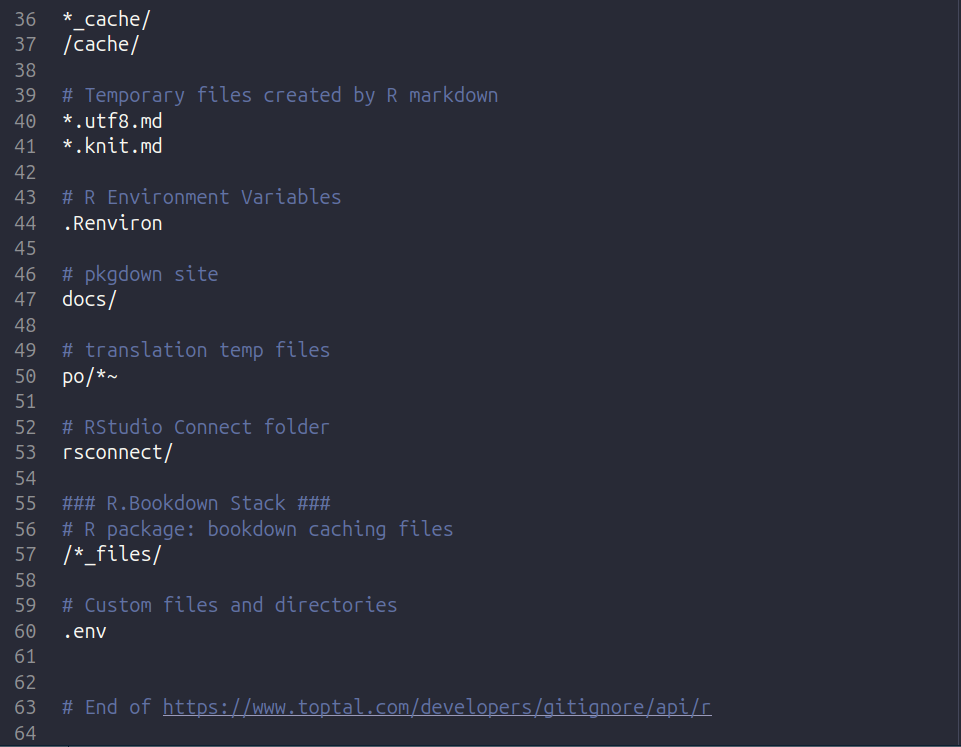
\includegraphics{images/git-ignore-env.png}
You are now ready to start downloading data!

\section{Organize your Project Directory}\label{organize-your-project-directory}

In your project directory create the following folders to organize your files:

\begin{itemize}
\tightlist
\item
  src - where you store your \texttt{.R} scripts
\item
  data - store downloaded data from CTT and modified dataframes
\item
  results - store plots made with \texttt{ggplot2}
\end{itemize}

\chapter{Download Data}\label{download-data}

You can download the following file types:

\begin{itemize}
\tightlist
\item
  raw: 434 MHz tag detections
\item
  blu: 2.4 GHz tag detections
\item
  gps: Sensor Station lat/lon with timestamps
\item
  node\_health: data on node battery, temperature, tag detections, etc.
\item
  telemetry: ???
\item
  sensorgnome: 166 MHz tag detections (Motus will need to translate the data into something usable)
\item
  log: Sensor Station log files
\end{itemize}

Trying to load all the data files into RStudio's memory will lead to issues, namely maxing out on memory usage. Instead, you should create an SQL relational database. Using a database uses much less memory when combining or cleaning data frames compared to loading data directly into RStudio, which leaves more memory for analyses.

If you are new to relational databases, you should use \href{https://duckdb.org/why_duckdb}{DuckDB}, a simple database management systems (DMBS) that is easy to install and use in RStudio.

\begin{Shaded}
\begin{Highlighting}[]
\CommentTok{\# activate renv environment}
\NormalTok{renv}\SpecialCharTok{::}\FunctionTok{activate}\NormalTok{()}
\end{Highlighting}
\end{Shaded}

The \texttt{celltracktech} package includes all the packages you need. Download it from github using \texttt{renv}.

\textbf{!NOTE} The DuckDB install will take \textasciitilde{} 30 min. Please allocate time accordingly.

\begin{Shaded}
\begin{Highlighting}[]
\CommentTok{\# install the celltracktech package using renv}
\FunctionTok{library}\NormalTok{(renv)}

\NormalTok{renv}\SpecialCharTok{::}\FunctionTok{install}\NormalTok{(}\StringTok{\textquotesingle{}cellular{-}tracking{-}technologies/celltracktech\textquotesingle{}}\NormalTok{)}
\end{Highlighting}
\end{Shaded}

If you want to download just your data files (in .csv.gz format), you can run the following script:

\begin{Shaded}
\begin{Highlighting}[]
\CommentTok{\# load the celltracktech library}
\FunctionTok{library}\NormalTok{(celltracktech)}

\CommentTok{\# load env file into environment}
\FunctionTok{load\_dot\_env}\NormalTok{(}\AttributeTok{file=}\StringTok{\textquotesingle{}.env\textquotesingle{}}\NormalTok{)}

\CommentTok{\# Settings {-}{-}{-}{-}{-}{-}{-}{-}{-}{-}{-}{-}{-}{-}{-}{-}{-}{-}{-}{-}{-}{-}{-}{-}{-}{-}{-}{-}{-}{-}{-}{-}{-}{-}{-}{-}{-}{-}{-}{-}{-}{-}{-}{-}{-}{-}{-}{-}{-}{-}{-}{-}{-}{-}{-}{-}{-}{-}{-}{-}{-}{-}{-}{-}}
\NormalTok{my\_token }\OtherTok{\textless{}{-}} \FunctionTok{Sys.getenv}\NormalTok{(}\StringTok{\textquotesingle{}API\_KEY\textquotesingle{}}\NormalTok{) }\CommentTok{\# load env variable into my\_token}
\NormalTok{myproject }\OtherTok{\textless{}{-}} \StringTok{"Meadows V2"} \CommentTok{\# this is your project name on your CTT account, here we are using the CTT project \textquotesingle{}Meadows V2\textquotesingle{}}

\CommentTok{\# Create your data directory if it does not exist}
\NormalTok{outpath }\OtherTok{\textless{}{-}} \StringTok{"./data/"} \CommentTok{\# where your downloaded files are to go}

\CommentTok{\# Create project name folder}
\FunctionTok{create\_outpath}\NormalTok{(}\FunctionTok{paste0}\NormalTok{(outpath, myproject, }\StringTok{\textquotesingle{}/\textquotesingle{}}\NormalTok{))}

\CommentTok{\# Download just the data files onto your computer}
\FunctionTok{get\_my\_data}\NormalTok{(}\AttributeTok{my\_token =}\NormalTok{ my\_token,}
            \AttributeTok{outpath =}\NormalTok{ outpath, }
            \AttributeTok{db\_name =} \ConstantTok{NULL}\NormalTok{,}
            \AttributeTok{myproject =}\NormalTok{ myproject,}
            \AttributeTok{begin =} \FunctionTok{as.Date}\NormalTok{(}\StringTok{"2023{-}08{-}01"}\NormalTok{),}
            \AttributeTok{end =} \FunctionTok{as.Date}\NormalTok{(}\StringTok{"2023{-}12{-}31"}\NormalTok{),}
            \AttributeTok{filetypes=}\FunctionTok{c}\NormalTok{(}\StringTok{"raw"}\NormalTok{, }\StringTok{"blu"}\NormalTok{, }\StringTok{"gps"}\NormalTok{, }\StringTok{"node\_health"}\NormalTok{, }\StringTok{"sensorgnome"}\NormalTok{, }\StringTok{"telemetry"}\NormalTok{, }\StringTok{\textquotesingle{}log\textquotesingle{}}\NormalTok{)}
\NormalTok{)}
\end{Highlighting}
\end{Shaded}

\section{Create a DuckDB database}\label{create-a-duckdb-database}

Below is a sample script to create a DuckDB database

\begin{Shaded}
\begin{Highlighting}[]
\CommentTok{\# Connect to Database using DuckDB {-}{-}{-}{-}{-}{-}{-}{-}{-}{-}{-}{-}{-}{-}{-}{-}{-}{-}{-}{-}{-}{-}{-}{-}{-}{-}{-}{-}{-}{-}{-}{-}{-}{-}{-}{-}{-}{-}{-}{-}{-}{-}{-}{-}{-}{-}{-}{-}{-}{-}{-}{-}{-}}
\NormalTok{con }\OtherTok{\textless{}{-}}\NormalTok{ DBI}\SpecialCharTok{::}\FunctionTok{dbConnect}\NormalTok{(duckdb}\SpecialCharTok{::}\FunctionTok{duckdb}\NormalTok{(), }
                      \AttributeTok{dbdir =} \StringTok{"./data/Meadows V2/meadows.duckdb"}\NormalTok{, }
                      \AttributeTok{read\_only =} \ConstantTok{FALSE}\NormalTok{)}
\end{Highlighting}
\end{Shaded}

\section{Download data from the CTT API}\label{download-data-from-the-ctt-api}

You are now connected to your DuckDB database, but so far nothing is in the database. The script below will download your data from the CTT servers. If you do not want to use a database, you can still use the \texttt{get\_my\_data()} function to download the .csv.gz files.

NOTE! Your Sensor Station must be set to upload data to our servers. If your station does not upload data, skip this block and go to section 2.2.1.

\begin{Shaded}
\begin{Highlighting}[]
\FunctionTok{get\_my\_data}\NormalTok{(}\AttributeTok{my\_token =}\NormalTok{ my\_token,}
            \AttributeTok{outpath =}\NormalTok{ outpath, }
            \AttributeTok{db\_name =}\NormalTok{ con, }
            \AttributeTok{myproject =}\NormalTok{ myproject,}
            \AttributeTok{begin =} \FunctionTok{as.Date}\NormalTok{(}\StringTok{"2023{-}08{-}01"}\NormalTok{),}
            \AttributeTok{end =} \FunctionTok{as.Date}\NormalTok{(}\StringTok{"2023{-}12{-}31"}\NormalTok{),}
            \AttributeTok{filetypes=}\FunctionTok{c}\NormalTok{(}\StringTok{"raw"}\NormalTok{, }\StringTok{"blu"}\NormalTok{, }\StringTok{"gps"}\NormalTok{, }\StringTok{"node\_health"}\NormalTok{, }\StringTok{"sensorgnome"}\NormalTok{, }\StringTok{"telemetry"}\NormalTok{, }\StringTok{\textquotesingle{}log\textquotesingle{}}\NormalTok{)}
\NormalTok{)}
\end{Highlighting}
\end{Shaded}

You may get this error message:

\begin{Shaded}
\begin{Highlighting}[]
\ExtensionTok{Error}\NormalTok{ in post}\ErrorTok{(}\ExtensionTok{endpoint}\NormalTok{ = endpoint, payload = payload}\KeywordTok{)} \BuiltInTok{:} 
  \ExtensionTok{Gateway}\NormalTok{ Timeout }\ErrorTok{(}\ExtensionTok{HTTP}\NormalTok{ 504}\KeywordTok{)}\BuiltInTok{.}
\end{Highlighting}
\end{Shaded}

It is fine, just run the \texttt{get\_my\_data()} function again and it should work properly.

\subsection{Create Database from Files on your Computer}\label{create-database-from-files-on-your-computer}

If you already have your Sensor Station files on your computer (i.e.~your sensor station is not connected to the internet), you can use the code block below to create a database and add those files to it.

\begin{Shaded}
\begin{Highlighting}[]
\NormalTok{celltracktech}\SpecialCharTok{::}\FunctionTok{create\_database}\NormalTok{(}\AttributeTok{my\_token =}\NormalTok{ my\_token,}
                               \AttributeTok{outpath =}\NormalTok{ outpath,}
                               \AttributeTok{myproject =}\NormalTok{ myproject,}
                               \AttributeTok{db\_name =}\NormalTok{ con)}
\end{Highlighting}
\end{Shaded}

\section{Updating the database}\label{updating-the-database}

Upload the compressed data (i.e.~the `.csv.gz' files) into your DuckDB database:

\begin{Shaded}
\begin{Highlighting}[]
\FunctionTok{update\_db}\NormalTok{(con, outpath, myproject)}
\end{Highlighting}
\end{Shaded}

\section{Disconnecting from the database}\label{disconnecting-from-the-database}

The benefit of using a relational database is that it does not need to be loaded into your computer memory the entire time you are analyzing your data. You can connect to it, filter/clean the data you want, and then disconnect once you are done, freeing up computer memory for more intensive data analysis tasks.

To disconnect from the database, run the following command:

\begin{Shaded}
\begin{Highlighting}[]
\NormalTok{DBI}\SpecialCharTok{::}\FunctionTok{dbDisconnect}\NormalTok{(con)}
\end{Highlighting}
\end{Shaded}

\section{Uploading Node Data from the SD Card}\label{uploading-node-data-from-the-sd-card}

\textbf{Note! This step is optional! If you are not uploading data from the Node SD cards, you can skip to chapter 3!}

\subsection{Create Nodes directory}\label{create-nodes-directory}

To upload Node data from the SD cards, you will need to create a `nodes' folder in the CTT Project Name folder. For example, we will create a folder in the `Meadows V2' folder in the `./data/meadows/' directory:

\begin{Shaded}
\begin{Highlighting}[]
\FunctionTok{create\_outpath}\NormalTok{(}\StringTok{\textquotesingle{}./data/Meadows V2/nodes/\textquotesingle{}}\NormalTok{)}
\end{Highlighting}
\end{Shaded}

\subsection{Create individual directories for each Node}\label{create-individual-directories-for-each-node}

Then, create a folder for each Node. In the example below, we are creating a folder for Node 3B8845:

\begin{Shaded}
\begin{Highlighting}[]
\FunctionTok{create\_outpath}\NormalTok{(}\StringTok{\textquotesingle{}./data/Meadows V2/nodes/3B8845/\textquotesingle{}}\NormalTok{)}
\end{Highlighting}
\end{Shaded}

If you are only uploading data from the node SD cards frequently, you should create a parent folder for the date you removed the data from the SD card. The nodes save files incrementally (i.e.~434\_mhz\_beep\_0, 434\_mhz\_beep1, etc.). If you remove the files, it will start back at 0 again. When you put the files with the same name in the same folder, one of them will be overwritten.

\begin{Shaded}
\begin{Highlighting}[]
\FunctionTok{create\_outpath}\NormalTok{(}\StringTok{\textquotesingle{}./data/Meadows V2/nodes/20250423/3B8845)\textquotesingle{}}\NormalTok{)}
\end{Highlighting}
\end{Shaded}

\subsection{Upload Node data to your DuckDB database}\label{upload-node-data-to-your-duckdb-database}

Remember, we need to re-connect to the DuckDB database to upload the Node data:

\begin{Shaded}
\begin{Highlighting}[]
\NormalTok{con }\OtherTok{\textless{}{-}}\NormalTok{ DBI}\SpecialCharTok{::}\FunctionTok{dbConnect}\NormalTok{(duckdb}\SpecialCharTok{::}\FunctionTok{duckdb}\NormalTok{(), }
                      \AttributeTok{dbdir =} \StringTok{"./data/Meadows V2/meadows.duckdb"}\NormalTok{, }
                      \AttributeTok{read\_only =} \ConstantTok{FALSE}\NormalTok{)}

\CommentTok{\# Import node data into your database}
\FunctionTok{import\_node\_data}\NormalTok{(}\AttributeTok{d =}\NormalTok{ con,}
                 \AttributeTok{outpath =}\NormalTok{ outpath,}
                 \AttributeTok{myproject =}\NormalTok{ myproject,}
                 \AttributeTok{station\_id =} \StringTok{\textquotesingle{}6CA25D375881\textquotesingle{}}\NormalTok{)}

\CommentTok{\# disconnect from the database}
\NormalTok{DBI}\SpecialCharTok{::}\FunctionTok{dbDisconnect}\NormalTok{(con)}
\end{Highlighting}
\end{Shaded}

If you get \texttt{Error\ in\ files\_loc{[}1,\ {]}\ :\ incorrect\ number\ of\ dimensions} you did not create the \texttt{nodes} folder in the correct location.

The \texttt{import\_node\_data} will import the node csv files into their own `node' tables

\begin{itemize}
\tightlist
\item
  node\_raw
\item
  node\_blu
\item
  node\_gps
\item
  node\_health\_from\_node
\end{itemize}

and insert the csv files into the regular ``raw'', ``blu'', and ``node\_health'' tables.

You have finished uploading data to your database!

\section{Create Postgres Database}\label{create-postgres-database}

If you or your lab are familiar with PostgreSQL, you can connect to your database with this:

\begin{Shaded}
\begin{Highlighting}[]
\CommentTok{\# connect to Postgres database}
\NormalTok{con }\OtherTok{\textless{}{-}}\NormalTok{ DBI}\SpecialCharTok{::}\FunctionTok{dbConnect}\NormalTok{(}
\NormalTok{  RPostgres}\SpecialCharTok{::}\FunctionTok{Postgres}\NormalTok{(),}
  \AttributeTok{dbname=}\StringTok{"meadows"}
\NormalTok{)}
\end{Highlighting}
\end{Shaded}

Creating and editing a Postgres database is vastly different from a DuckDB database. You can find more information on Postgres and R \href{https://faculty.washington.edu/phurvitz/r_sql/createdb.html}{here}.

You should be able to do all the above as long as you use \texttt{RPostgres::Postgres()} in your database connection.

\chapter{Obtaining Data from Database}\label{obtaining-data-from-database}

\section{Duckplyr}\label{duckplyr}

If you are new to database queries but familiar with \texttt{dplyr} and \texttt{tidyverse}, we recommend using \texttt{duckplyr}. You can find more information about \texttt{duckplyr} \href{https://duckdb.org/2024/04/02/duckplyr.html}{here} but the main takeaway is that you can query your database using dplyr phrases and pipes, while also saving memory on loading data.

\begin{Shaded}
\begin{Highlighting}[]
\FunctionTok{library}\NormalTok{(celltracktech)}

\NormalTok{con }\OtherTok{\textless{}{-}}\NormalTok{ DBI}\SpecialCharTok{::}\FunctionTok{dbConnect}\NormalTok{(duckdb}\SpecialCharTok{::}\FunctionTok{duckdb}\NormalTok{(), }
                      \AttributeTok{dbdir =} \StringTok{"./data/Meadows V2/meadows.duckdb"}\NormalTok{, }
                      \AttributeTok{read\_only =} \ConstantTok{FALSE}\NormalTok{)}

\CommentTok{\# load raw data table and find unique tags}
\NormalTok{unique\_tags }\OtherTok{=} \FunctionTok{tbl}\NormalTok{(con, }\StringTok{\textquotesingle{}raw\textquotesingle{}}\NormalTok{) }\SpecialCharTok{|\textgreater{}} 
  \FunctionTok{group\_by}\NormalTok{(tag\_id) }\SpecialCharTok{|\textgreater{}}
  \FunctionTok{summarize}\NormalTok{(}\AttributeTok{num\_detect =} \FunctionTok{n}\NormalTok{()) }\SpecialCharTok{|\textgreater{}}
  \FunctionTok{select}\NormalTok{(tag\_id, num\_detect) }\SpecialCharTok{|\textgreater{}}
  \FunctionTok{arrange}\NormalTok{(}\FunctionTok{desc}\NormalTok{(num\_detect)) }\SpecialCharTok{|\textgreater{}}
  \FunctionTok{collect}\NormalTok{()}

\NormalTok{DBI}\SpecialCharTok{::}\FunctionTok{dbDisconnect}\NormalTok{(con)}
\end{Highlighting}
\end{Shaded}

\section{SQL Queries}\label{sql-queries}

If you are more comfortable with the SQL syntax, you can use SQL queries to get data from different tables.

This chapter is a quick summary on how to use SQL in R. If you would like more info on how to run different queries, use this tutorial: \url{https://solutions.posit.co/connections/db/getting-started/database-queries/}

\section{List Tables}\label{list-tables}

List the tables in your database. If everything was run correctly, each data file type (raw, blu, node-health, etc.) should be in its own data table.

Remember to reconnect to the database!

\begin{Shaded}
\begin{Highlighting}[]
\FunctionTok{library}\NormalTok{(celltracktech)}

\NormalTok{con }\OtherTok{\textless{}{-}}\NormalTok{ DBI}\SpecialCharTok{::}\FunctionTok{dbConnect}\NormalTok{(duckdb}\SpecialCharTok{::}\FunctionTok{duckdb}\NormalTok{(), }
                      \AttributeTok{dbdir =} \StringTok{"./data/Meadows V2/meadows.duckdb"}\NormalTok{, }
                      \AttributeTok{read\_only =} \ConstantTok{FALSE}\NormalTok{)}

\CommentTok{\# list tables in database}
\NormalTok{DBI}\SpecialCharTok{::}\FunctionTok{dbListTables}\NormalTok{(con)}

\CommentTok{\# disconnect from database}
\NormalTok{DBI}\SpecialCharTok{::}\FunctionTok{dbDisconnect}\NormalTok{(con)}
\end{Highlighting}
\end{Shaded}

\section{\texorpdfstring{Find unique tags in \texttt{raw} table}{Find unique tags in raw table}}\label{find-unique-tags-in-raw-table}

\begin{Shaded}
\begin{Highlighting}[]
\CommentTok{\# connect to database}
\NormalTok{con }\OtherTok{\textless{}{-}}\NormalTok{ DBI}\SpecialCharTok{::}\FunctionTok{dbConnect}\NormalTok{(duckdb}\SpecialCharTok{::}\FunctionTok{duckdb}\NormalTok{(), }
                      \AttributeTok{dbdir =} \StringTok{"./data/Meadows V2/meadows.duckdb"}\NormalTok{, }
                      \AttributeTok{read\_only =} \ConstantTok{FALSE}\NormalTok{)}

\CommentTok{\# list last 10 records in raw}
\NormalTok{raw }\OtherTok{=}\NormalTok{ DBI}\SpecialCharTok{::}\FunctionTok{dbGetQuery}\NormalTok{(con, }\StringTok{"SELECT * FROM raw}
\StringTok{                           ORDER BY time DESC}
\StringTok{                           LIMIT 10"}\NormalTok{)}
\NormalTok{raw}

\CommentTok{\# find unique tags in the raw table}
\NormalTok{unique\_tag }\OtherTok{=} \FunctionTok{dbGetQuery}\NormalTok{(con,}
                        \StringTok{\textquotesingle{}SELECT tag\_id, COUNT(*) AS num\_detect}
\StringTok{                        FROM raw}
\StringTok{                        GROUP BY tag\_id}
\StringTok{                        ORDER BY num\_detect DESC\textquotesingle{}}\NormalTok{)}
\NormalTok{DBI}\SpecialCharTok{::}\FunctionTok{dbDisconnect}\NormalTok{(con)}
\end{Highlighting}
\end{Shaded}

Note: you do not need to load each table into RStudio. You should only load the tables you need to for your analysis.

\chapter{Node Check}\label{node-check}

With your data you can run the following analyses:

\begin{itemize}
\tightlist
\item
  Presence/absence using detection times
\item
  Activity budget using the change in signal strength over time
\item
  Habitat Use using localization
\item
  Home range/territory size
\item
  Movement patterns
\end{itemize}

Before you can do any of that, it is a good idea to check if your nodes are working properly, and filter out any that are malfunctioning.

\section{Node Health}\label{node-health}

Things to look at:

\begin{itemize}
\tightlist
\item
  Recent health records and detections
\item
  Battery Level
\item
  Are they charging?
\item
  GPS fixes
\item
  Synchronized clocks?
\end{itemize}

For example, debris on solar panels can lead to the node not to charge, which means the battery voltage will drop, which stops the GPS, leading to an out of sync clock.

Another example is that foliage cover leads to no charging, low battery voltage, stops the GPS, and leads to an out of sync clock.

\subsection{Node Health - Check Health Records}\label{node-health---check-health-records}

\subsubsection{Load Data from Database}\label{load-data-from-database}

\begin{Shaded}
\begin{Highlighting}[]
\FunctionTok{library}\NormalTok{(celltracktech)}

\CommentTok{\# load env file into environment}
\FunctionTok{load\_dot\_env}\NormalTok{(}\AttributeTok{file=}\StringTok{\textquotesingle{}.env\textquotesingle{}}\NormalTok{)}

\CommentTok{\# Settings {-} {-}{-}{-}{-}{-}{-}{-}{-}{-}{-}{-}{-}{-}{-}{-}{-}{-}{-}{-}{-}{-}{-}{-}{-}{-}{-}{-}{-}{-}{-}{-}{-}{-}{-}{-}{-}{-}{-}{-}{-}{-}{-}{-}{-}{-}{-}{-}{-}{-}{-}{-}{-}{-}{-}{-}{-}{-}{-}{-}{-}{-}{-}{-}{-}}
\CommentTok{\# These were created in Chapter 2. If you do not have these in your project directory, go back and repeat Ch. 2.}
\NormalTok{my\_token }\OtherTok{\textless{}{-}} \FunctionTok{Sys.getenv}\NormalTok{(}\StringTok{\textquotesingle{}API\_KEY\textquotesingle{}}\NormalTok{) }\CommentTok{\# load env variable into my\_token}
\NormalTok{myproject }\OtherTok{\textless{}{-}} \StringTok{"Meadows V2"} \CommentTok{\# this is your project name on your CTT account, here we are using the CTT project \textquotesingle{}Meadows V2\textquotesingle{}}
\NormalTok{outpath }\OtherTok{\textless{}{-}} \StringTok{"./data/"} \CommentTok{\# where your downloaded files are to go}

\CommentTok{\# Specify the time range of node data you want to import for this analysis}
\NormalTok{start\_time }\OtherTok{\textless{}{-}} \FunctionTok{as.POSIXct}\NormalTok{(}\StringTok{"2023{-}08{-}01 00:00:00"}\NormalTok{, }\AttributeTok{tz =} \StringTok{"GMT"}\NormalTok{)}
\NormalTok{stop\_time }\OtherTok{\textless{}{-}} \FunctionTok{as.POSIXct}\NormalTok{(}\StringTok{"2023{-}08{-}07 00:00:00"}\NormalTok{, }\AttributeTok{tz =} \StringTok{"GMT"}\NormalTok{)}

\CommentTok{\# Connect to Database using DuckDB {-}{-}{-}{-}{-}{-}{-}{-}{-}{-}{-}{-}{-}{-}{-}{-}{-}{-}{-}{-}{-}{-}{-}{-}{-}{-}{-}{-}{-}{-}{-}{-}{-}{-}{-}{-}{-}{-}{-}{-}{-}{-}{-}{-}{-}{-}{-}{-}{-}{-}{-}{-}{-}}
\NormalTok{con }\OtherTok{\textless{}{-}}\NormalTok{ DBI}\SpecialCharTok{::}\FunctionTok{dbConnect}\NormalTok{(duckdb}\SpecialCharTok{::}\FunctionTok{duckdb}\NormalTok{(), }
                      \AttributeTok{dbdir =} \StringTok{"./data/Meadows V2/meadows.duckdb"}\NormalTok{, }
                      \AttributeTok{read\_only =} \ConstantTok{FALSE}\NormalTok{)}

\CommentTok{\# load node\_health table into RStudio and only load the data between the set start and stop times}
\NormalTok{node\_health\_df }\OtherTok{\textless{}{-}} \FunctionTok{tbl}\NormalTok{(con, }\StringTok{"node\_health"}\NormalTok{) }\SpecialCharTok{|\textgreater{}} 
  \FunctionTok{filter}\NormalTok{(time }\SpecialCharTok{\textgreater{}=}\NormalTok{ start\_time }\SpecialCharTok{\&}\NormalTok{ time }\SpecialCharTok{\textless{}=}\NormalTok{ stop\_time) }\SpecialCharTok{|\textgreater{}}
  \FunctionTok{collect}\NormalTok{()}

\CommentTok{\# disconnect from database}
\NormalTok{DBI}\SpecialCharTok{::}\FunctionTok{dbDisconnect}\NormalTok{(con)}

\CommentTok{\# filter the node\_health\_df for unique node ids}
\NormalTok{node\_health\_df }\OtherTok{\textless{}{-}}\NormalTok{ node\_health\_df }\SpecialCharTok{|\textgreater{}}
  \FunctionTok{distinct}\NormalTok{(node\_id, }
\NormalTok{            time, }
\NormalTok{            recorded\_at, }
            \AttributeTok{.keep\_all =} \ConstantTok{TRUE}\NormalTok{)}
\end{Highlighting}
\end{Shaded}

\subsubsection{Check if nodes are operating properly}\label{check-if-nodes-are-operating-properly}

\begin{Shaded}
\begin{Highlighting}[]
\CommentTok{\# Look at the number of health records received from each node}
\NormalTok{node\_record\_counts }\OtherTok{\textless{}{-}}\NormalTok{ node\_health\_df }\SpecialCharTok{\%\textgreater{}\%} \FunctionTok{count}\NormalTok{(node\_id)}

\CommentTok{\# sort the node\_record\_counts by decreasing number}
\NormalTok{node\_record\_counts }\OtherTok{\textless{}{-}}\NormalTok{ node\_record\_counts[}\FunctionTok{order}\NormalTok{(node\_record\_counts}\SpecialCharTok{$}\NormalTok{n, }\AttributeTok{decreasing =} \ConstantTok{TRUE}\NormalTok{),]}

\CommentTok{\# plot the number of node health records based on node id}
\FunctionTok{ggplot}\NormalTok{(node\_record\_counts,}
       \FunctionTok{aes}\NormalTok{(}\AttributeTok{x =} \FunctionTok{factor}\NormalTok{(}\AttributeTok{x =}\NormalTok{ node\_id,}
                      \AttributeTok{levels =}\NormalTok{ node\_id),}
           \AttributeTok{y =}\NormalTok{ n)) }\SpecialCharTok{+}
  \FunctionTok{geom\_bar}\NormalTok{(}\AttributeTok{stat =} \StringTok{"identity"}\NormalTok{) }\SpecialCharTok{+}
  \FunctionTok{coord\_flip}\NormalTok{() }\SpecialCharTok{+}
  \FunctionTok{labs}\NormalTok{(}\AttributeTok{x =} \StringTok{"Health Record Count"}\NormalTok{,}
       \AttributeTok{y =} \StringTok{"Node Id"}\NormalTok{) }\SpecialCharTok{+}
  \FunctionTok{tag\_hist\_plot\_theme}\NormalTok{()}
\end{Highlighting}
\end{Shaded}

\begin{figure}
\centering
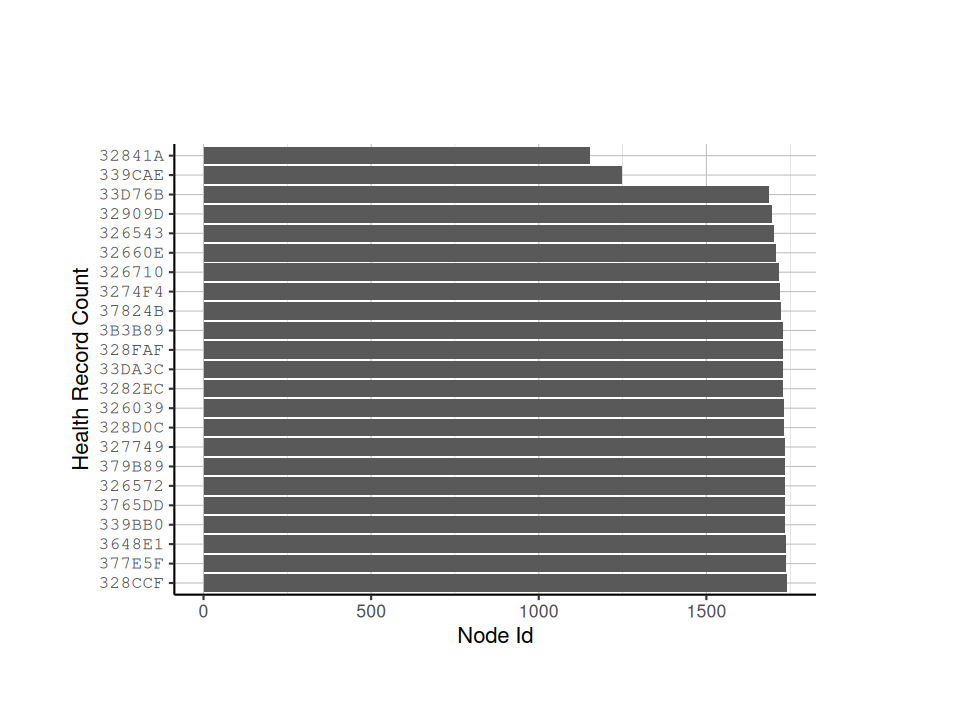
\includegraphics{images/node_check_1.1.2_check_if_nodes_are_operating_properly.png}
\caption{Plot of node health record counts}
\end{figure}

We can see after running the above script that Nodes 339CAE and 32841A have relatively low number of records, so we may want to exclude them from further analyses.

\subsection{Battery and Solar Levels}\label{battery-and-solar-levels}

Check if the battery and solar voltages are adequate. If they are too low, they can affect the GPS synchronization.

\begin{Shaded}
\begin{Highlighting}[]
\CommentTok{\# Plot the Battery voltage vs. time for all nodes}
\FunctionTok{ggplot}\NormalTok{(node\_health\_df) }\SpecialCharTok{+}
  \FunctionTok{geom\_point}\NormalTok{(}\FunctionTok{aes}\NormalTok{(}\AttributeTok{x =}\NormalTok{ time,}
                 \AttributeTok{y =}\NormalTok{ battery,}
                 \AttributeTok{colour =}\NormalTok{ node\_id)) }\SpecialCharTok{+}
  \FunctionTok{classic\_plot\_theme}\NormalTok{()}
\end{Highlighting}
\end{Shaded}

\begin{figure}
\centering
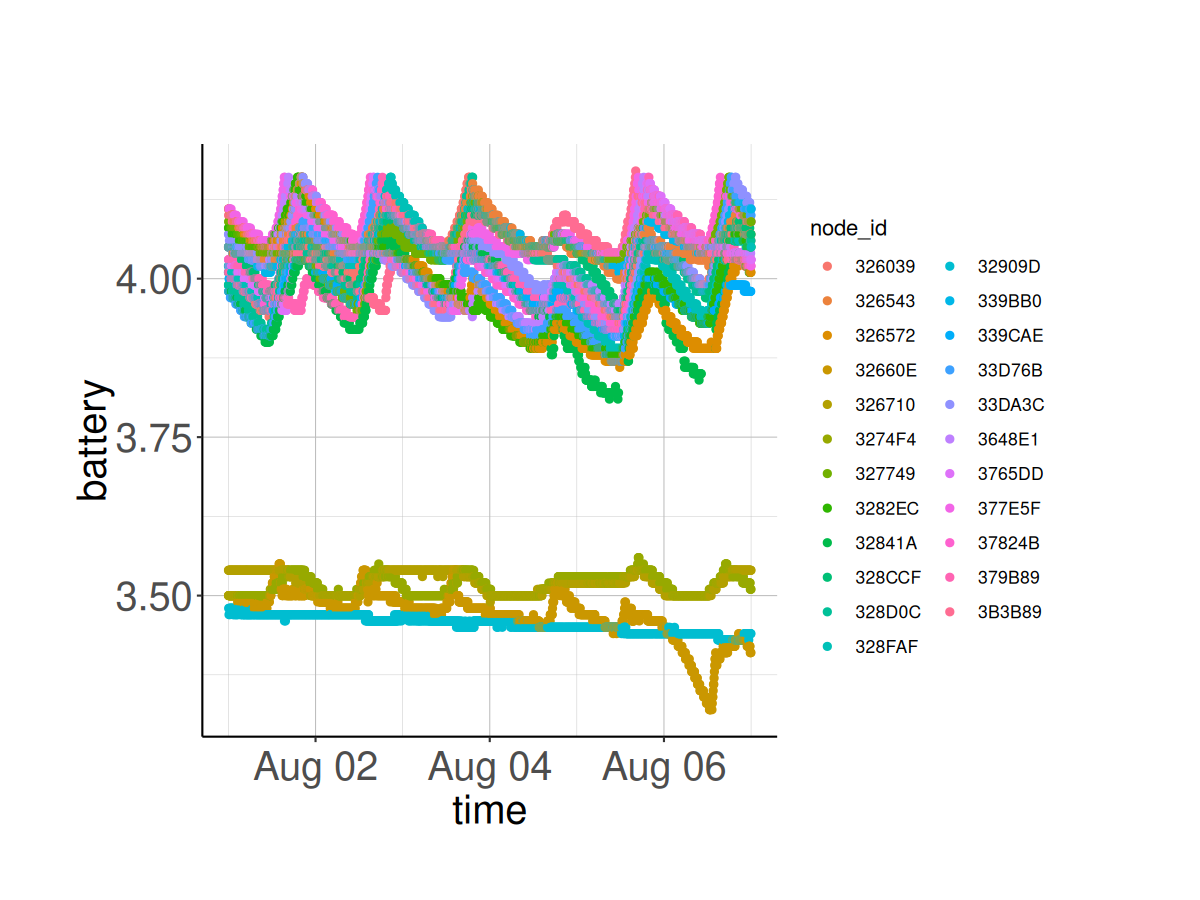
\includegraphics{images/node_check_1.1.3_battery_vs_time_all_nodes.png}
\caption{Plot of node battery voltage (V) vs.~time}
\end{figure}

\begin{Shaded}
\begin{Highlighting}[]
\CommentTok{\# Plot the Battery \& Solar voltage vs. time for a specific node}
\CommentTok{\# Node 326710 is a normal working Node}
\NormalTok{selected\_node\_id }\OtherTok{\textless{}{-}} \StringTok{"326710"}
\NormalTok{batt\_solar\_plot }\OtherTok{\textless{}{-}} \FunctionTok{plot\_battery\_solar}\NormalTok{(}\AttributeTok{node\_health\_df =}\NormalTok{ node\_health\_df, }
                                      \AttributeTok{selected\_node\_id =}\NormalTok{ selected\_node\_id)}
\NormalTok{batt\_solar\_plot }
\end{Highlighting}
\end{Shaded}

\begin{figure}
\centering
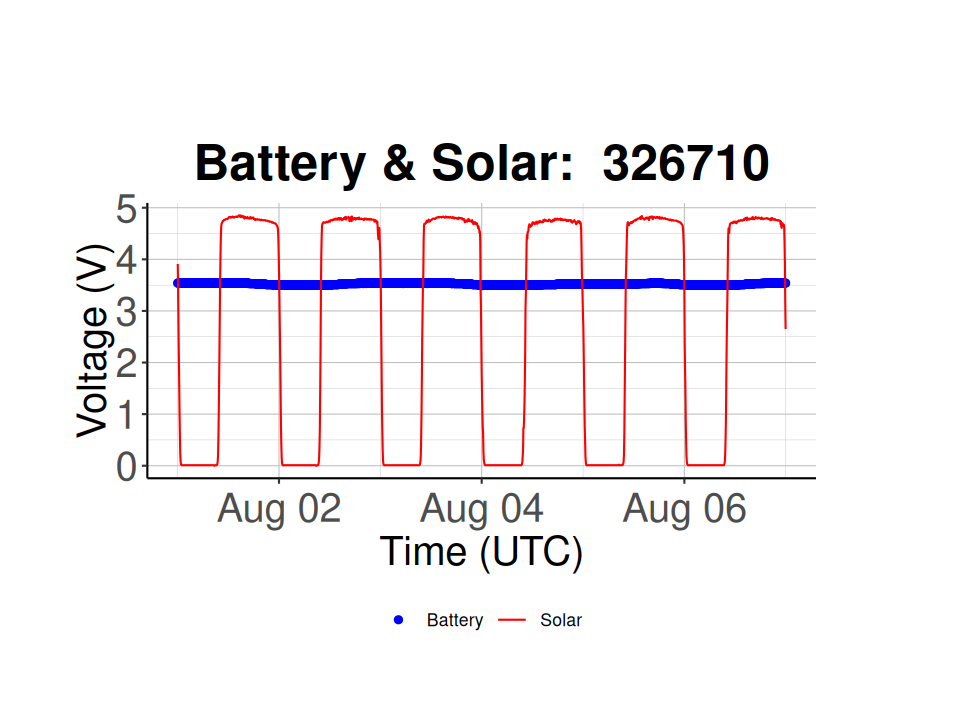
\includegraphics{images/node_check_1.1.3_node_specific_battery_solar_normal.png}
\caption{Plot of Battery and Solar voltage (V) vs.~time for a specific node}
\end{figure}

\begin{Shaded}
\begin{Highlighting}[]
\CommentTok{\# based on the Battery voltage vs. time plot, Node 32909D has a low battery voltage}
\NormalTok{selected\_node\_id }\OtherTok{\textless{}{-}} \StringTok{\textquotesingle{}32909D\textquotesingle{}}
\NormalTok{batt\_solar\_plot }\OtherTok{\textless{}{-}} \FunctionTok{plot\_battery\_solar}\NormalTok{(}\AttributeTok{node\_health\_df =}\NormalTok{ node\_health\_df, }
                                      \AttributeTok{selected\_node\_id =}\NormalTok{ selected\_node\_id)}
\NormalTok{batt\_solar\_plot }
\end{Highlighting}
\end{Shaded}

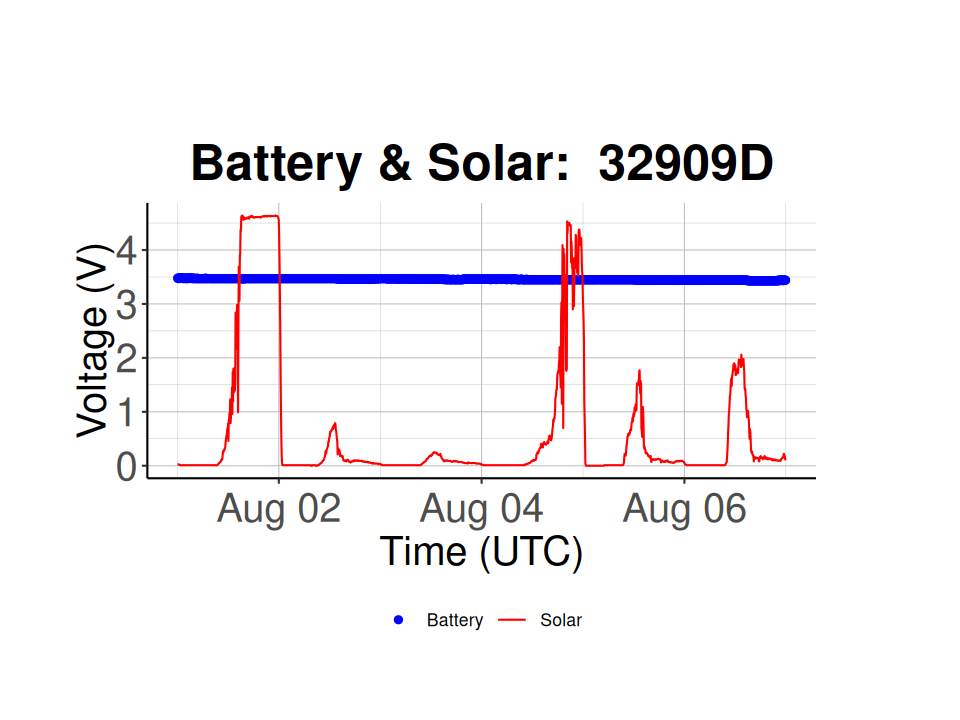
\includegraphics{images/node_check_1.1.3_node_specific_battery_solar_bad.png}
Node 326710 is working properly and has consistent solar voltages during the day (\textasciitilde{} 5 V) and a consistent battery voltage over time (i.e.~3.5-3.6 V), while node 32909D has inconsistent solar voltages, hinting at either dirty solar panels or covered solar panels, and a much lower battery voltage (\textasciitilde{} 2.8 V).

\subsection{Check GPS}\label{check-gps}

If the clock is out of sync, the GPS coordinates may not be calculated correctly. Use the below script to check the coordinate deviations.

\begin{Shaded}
\begin{Highlighting}[]
\CommentTok{\# calculate the node locations based on the latitude and longitude from node health reports}
\NormalTok{node\_locations }\OtherTok{\textless{}{-}} \FunctionTok{calculate\_node\_locations}\NormalTok{(node\_health\_df)}

\CommentTok{\# plot reported node locations and calculated node locations}
\FunctionTok{plot\_node\_locations}\NormalTok{(node\_health\_df, node\_locations)}

\CommentTok{\# looks like we have an outlier in our nodes list, let\textquotesingle{}s filter that out}
\CommentTok{\# filter meadows nodes due to outlier}
\NormalTok{nodes\_meadows }\OtherTok{=}\NormalTok{ node\_health\_df }\SpecialCharTok{\%\textgreater{}\%}
  \FunctionTok{filter}\NormalTok{(}\SpecialCharTok{!}\NormalTok{node\_id }\SpecialCharTok{\%in\%} \StringTok{\textquotesingle{}3B3B8F\textquotesingle{}}\NormalTok{) }\CommentTok{\# get data from all nodes EXCEPT node 3B3B8F}

\CommentTok{\# calculate the node locations based on the latitude and longitude from node health reports}
\NormalTok{node\_locations }\OtherTok{\textless{}{-}} \FunctionTok{calculate\_node\_locations}\NormalTok{(nodes\_meadows)}

\CommentTok{\# plot reported node locations and calculated node locations}
\FunctionTok{plot\_node\_locations}\NormalTok{(nodes\_meadows, node\_locations)}
\end{Highlighting}
\end{Shaded}

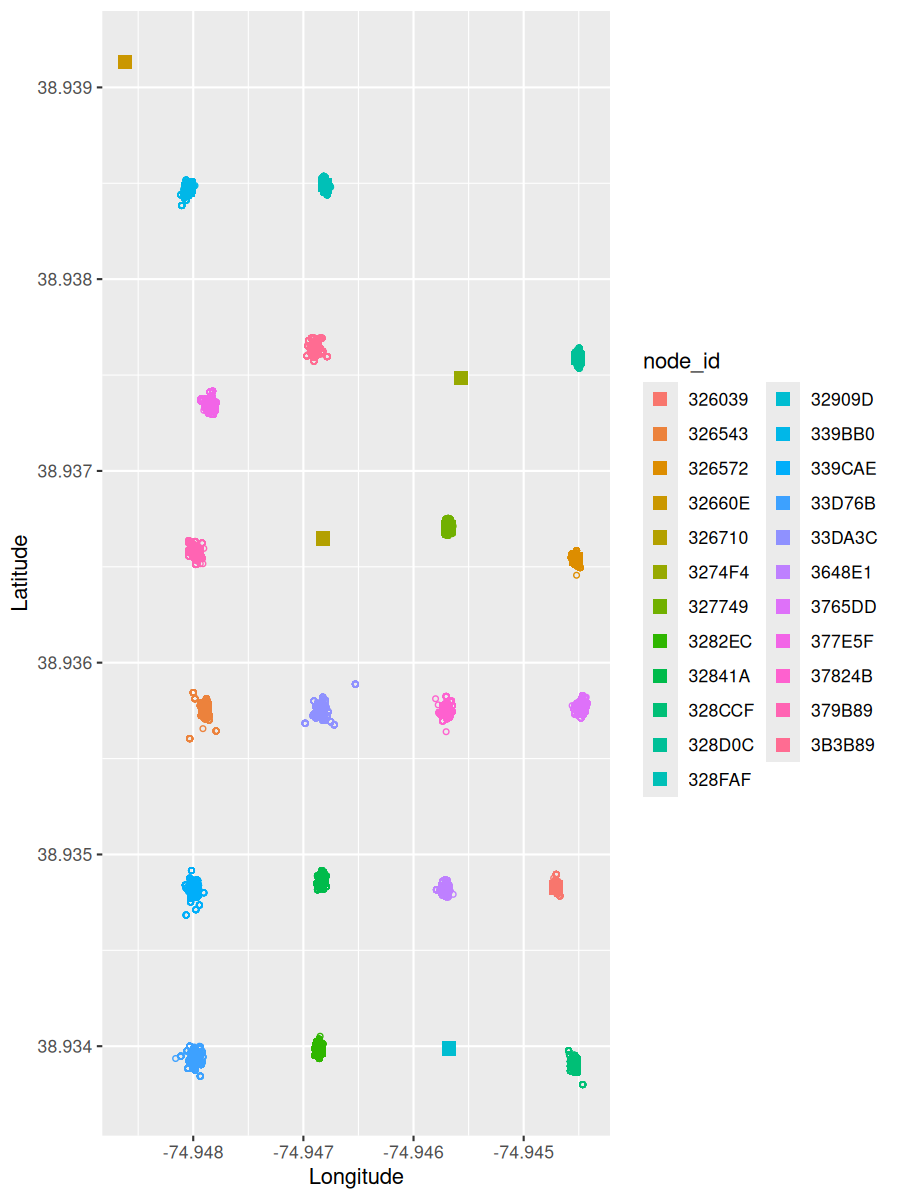
\includegraphics{images/node_check_1.3_node_locations.png}
\#\#\# Check Time Offset

Plot time offset for each node.

\begin{Shaded}
\begin{Highlighting}[]
\CommentTok{\# subtract time from recorded\_at, then calculate the average time offset for each node}
\NormalTok{node\_summary }\OtherTok{=}\NormalTok{ node\_health\_df }\SpecialCharTok{\%\textgreater{}\%}
  \FunctionTok{mutate}\NormalTok{(}\AttributeTok{time\_offset =}\NormalTok{ time}\SpecialCharTok{{-}}\NormalTok{recorded\_at) }\SpecialCharTok{\%\textgreater{}\%}
  \FunctionTok{group\_by}\NormalTok{(node\_id) }\SpecialCharTok{\%\textgreater{}\%}
  \FunctionTok{summarize}\NormalTok{(}\AttributeTok{mean\_time\_offset =} \FunctionTok{mean}\NormalTok{(time\_offset), }\AttributeTok{n =} \FunctionTok{n}\NormalTok{())}

\CommentTok{\# save node time offsets to csv}
\FunctionTok{write\_csv}\NormalTok{(node\_summary,}
                 \AttributeTok{file =} \StringTok{\textquotesingle{}./data/Meadows V2/node\_time\_offset\_20230802.csv\textquotesingle{}}\NormalTok{)}

\CommentTok{\# plot the time offset}
\FunctionTok{ggplot}\NormalTok{(node\_summary,}
       \FunctionTok{aes}\NormalTok{(}\AttributeTok{x =}\NormalTok{ node\_id, }
           \CommentTok{\# y = scale(mean\_time\_offset),}
           \AttributeTok{y =} \FunctionTok{as.numeric}\NormalTok{(mean\_time\_offset),}
           \AttributeTok{color=}\FunctionTok{factor}\NormalTok{(node\_id))) }\SpecialCharTok{+}
  \FunctionTok{geom\_point}\NormalTok{() }\SpecialCharTok{+}
  \FunctionTok{ggtitle}\NormalTok{(}\StringTok{"Time Offset"}\NormalTok{) }\SpecialCharTok{+}
  \FunctionTok{ylab}\NormalTok{(}\StringTok{"Time (s)"}\NormalTok{) }\SpecialCharTok{+}
  \FunctionTok{geom\_hline}\NormalTok{(}\AttributeTok{yintercept=}\DecValTok{0}\NormalTok{, }
             \AttributeTok{linetype=}\StringTok{"dotted"}\NormalTok{, }
             \AttributeTok{color =} \StringTok{"red"}\NormalTok{, }
             \AttributeTok{linewidth=}\DecValTok{1}\NormalTok{) }\SpecialCharTok{+}
  \FunctionTok{labs}\NormalTok{(}\AttributeTok{color =} \StringTok{\textquotesingle{}Node ID\textquotesingle{}}\NormalTok{) }\SpecialCharTok{+}
  \FunctionTok{classic\_plot\_theme}\NormalTok{() }\SpecialCharTok{+}
  \FunctionTok{theme}\NormalTok{(}\AttributeTok{axis.title.x =} \FunctionTok{element\_blank}\NormalTok{(),}
        \AttributeTok{axis.text.x=}\FunctionTok{element\_blank}\NormalTok{(),}
        \AttributeTok{axis.ticks.x=}\FunctionTok{element\_blank}\NormalTok{()}
\NormalTok{        )}
\end{Highlighting}
\end{Shaded}

\begin{figure}
\centering
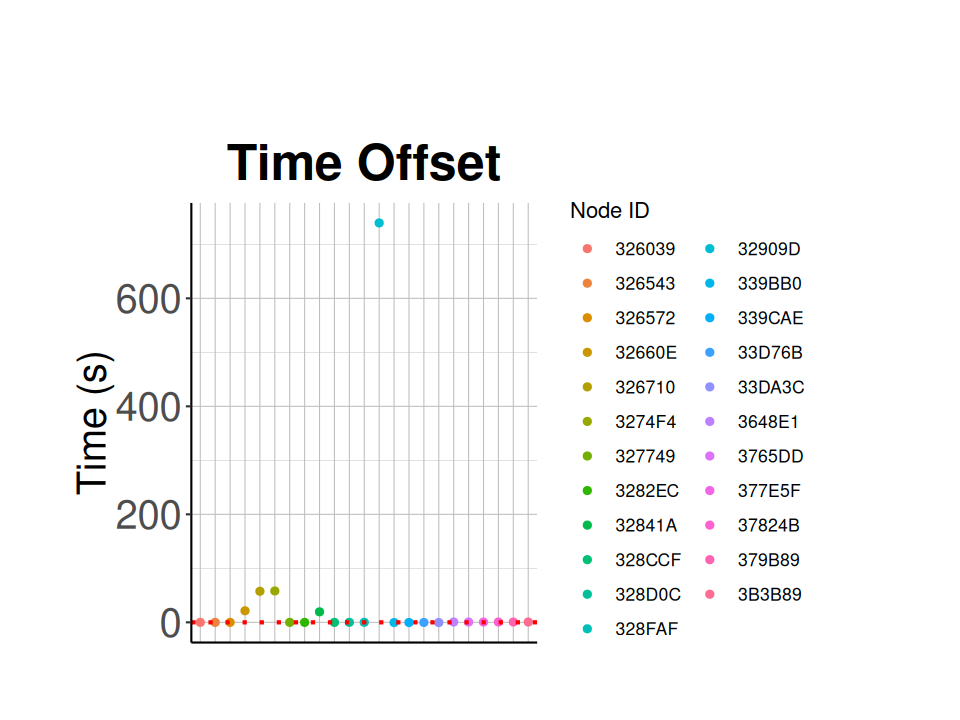
\includegraphics{images/node_check_1.4_time_offset.png}
\caption{Node time offset}
\end{figure}

\chapter{Node Calibration}\label{node-calibration}

In the previous chapter we saw that various ways that the node gps can differ, which can lead to inaccurate received signal strength indicators (RSSI) from the tag.

To account for any small changes in the gps values, we need to calibrate the node grid.
\#\# Load library

\begin{Shaded}
\begin{Highlighting}[]
\FunctionTok{library}\NormalTok{(celltracktech)}
\end{Highlighting}
\end{Shaded}

\section{Load sidekick data file}\label{load-sidekick-data-file}

Place the .csv file generated by the CTT Sidekick into the sidekick folder:

\begin{Shaded}
\begin{Highlighting}[]
\CommentTok{\# Specify the path to the sidekick data file you recorded for calibration}
\CommentTok{\# it is best if you create a \textquotesingle{}sidekick\textquotesingle{} folder to store your calibration file(s).}

\FunctionTok{create\_outpath}\NormalTok{(}\StringTok{\textquotesingle{}./data/Meadows V2/sidekick/\textquotesingle{}}\NormalTok{)}
\end{Highlighting}
\end{Shaded}

The \texttt{celltracktech} package comes with the sidekick calibration file from the Meadows V2 site. For the purposes of this tutorial, we will save it as a .csv file and place it in the sidekick folder. If you were using your data, you would need to place the sidekick calibration file manuall in the sidekick folder.

\begin{Shaded}
\begin{Highlighting}[]
\FunctionTok{write\_csv}\NormalTok{(celltracktech}\SpecialCharTok{::}\NormalTok{sidekick\_cal, }\StringTok{\textquotesingle{}./data/Meadows V2/sidekick/calibration.csv\textquotesingle{}}\NormalTok{)}

\NormalTok{sidekick\_file\_path }\OtherTok{\textless{}{-}} \StringTok{\textquotesingle{}./data/Meadows V2/sidekick/calibration.csv\textquotesingle{}}
\end{Highlighting}
\end{Shaded}

\subsection{IF YOU DO NOT HAVE A SIDEKICK DATA FILE:}\label{if-you-do-not-have-a-sidekick-data-file}

Create your own sidekick file by walking with a tag through node grid, stopping at specific spots you choose, and note the gps coordinates and time. Then create a csv similar to the sidekick calibration file.

Example:

\begin{longtable}[]{@{}
  >{\raggedright\arraybackslash}p{(\columnwidth - 14\tabcolsep) * \real{0.1698}}
  >{\raggedright\arraybackslash}p{(\columnwidth - 14\tabcolsep) * \real{0.1132}}
  >{\raggedright\arraybackslash}p{(\columnwidth - 14\tabcolsep) * \real{0.1509}}
  >{\raggedright\arraybackslash}p{(\columnwidth - 14\tabcolsep) * \real{0.0755}}
  >{\raggedright\arraybackslash}p{(\columnwidth - 14\tabcolsep) * \real{0.0566}}
  >{\raggedright\arraybackslash}p{(\columnwidth - 14\tabcolsep) * \real{0.0566}}
  >{\raggedright\arraybackslash}p{(\columnwidth - 14\tabcolsep) * \real{0.1321}}
  >{\raggedright\arraybackslash}p{(\columnwidth - 14\tabcolsep) * \real{0.2453}}@{}}
\toprule\noalign{}
\begin{minipage}[b]{\linewidth}\raggedright
tag\_type
\end{minipage} & \begin{minipage}[b]{\linewidth}\raggedright
tag\_id
\end{minipage} & \begin{minipage}[b]{\linewidth}\raggedright
time\_utc
\end{minipage} & \begin{minipage}[b]{\linewidth}\raggedright
rssi
\end{minipage} & \begin{minipage}[b]{\linewidth}\raggedright
lat
\end{minipage} & \begin{minipage}[b]{\linewidth}\raggedright
lon
\end{minipage} & \begin{minipage}[b]{\linewidth}\raggedright
heading
\end{minipage} & \begin{minipage}[b]{\linewidth}\raggedright
antenna\_angle
\end{minipage} \\
\midrule\noalign{}
\endhead
\bottomrule\noalign{}
\endlastfoot
radio434mhz & 4C34074B & 2023-08-03 19:42:44.721001Z & & 38.935561 & -74.948195 & 24.273 & \\
radio434mhz & 072A6633 & 2023-08-03 19:42:45.307456Z & & 38.935561 & -74.948195 & 23.548 & \\
radio434mhz & 19332A07 & 2023-08-03 19:42:48.366123Z & & 38.935569 & -74.948195 & 15.840 & \\
\end{longtable}

\section{Setup}\label{setup}

\subsection{Load environmental variables into RStudio}\label{load-environmental-variables-into-rstudio}

\begin{Shaded}
\begin{Highlighting}[]
\CommentTok{\# load env file into environment}
\FunctionTok{load\_dot\_env}\NormalTok{(}\AttributeTok{file=}\StringTok{\textquotesingle{}.env\textquotesingle{}}\NormalTok{)}
\end{Highlighting}
\end{Shaded}

\subsection{Load settings}\label{load-settings}

\begin{Shaded}
\begin{Highlighting}[]
\CommentTok{\# Settings {-} {-}{-}{-}{-}{-}{-}{-}{-}{-}{-}{-}{-}{-}{-}{-}{-}{-}{-}{-}{-}{-}{-}{-}{-}{-}{-}{-}{-}{-}{-}{-}{-}{-}{-}{-}{-}{-}{-}{-}{-}{-}{-}{-}{-}{-}{-}{-}{-}{-}{-}{-}{-}{-}{-}{-}{-}{-}{-}{-}{-}{-}{-}{-}{-}}

\CommentTok{\# set significant digits (number of digits after decimal)}
\FunctionTok{options}\NormalTok{(}\AttributeTok{digits =} \DecValTok{10}\NormalTok{)}

\CommentTok{\# These were created in Chapter 2. If you do not have these in your project directory, go back and repeat Ch. 2.}
\NormalTok{my\_token }\OtherTok{\textless{}{-}} \FunctionTok{Sys.getenv}\NormalTok{(}\StringTok{\textquotesingle{}API\_KEY\textquotesingle{}}\NormalTok{) }\CommentTok{\# load env variable into my\_token}
\NormalTok{myproject }\OtherTok{\textless{}{-}} \StringTok{"Meadows V2"} \CommentTok{\# this is your project name on your CTT account, here we are using the CTT project \textquotesingle{}Meadows V2\textquotesingle{}}
\NormalTok{outpath }\OtherTok{\textless{}{-}} \StringTok{"./data/"} \CommentTok{\# where your downloaded files are to go}

\CommentTok{\# Specify the path to your database file}
\NormalTok{database\_file }\OtherTok{\textless{}{-}} \StringTok{"./data/Meadows V2/meadows.duckdb"}

\CommentTok{\# Specify the tag ID that you used in your calibration}
\NormalTok{my\_tag\_id }\OtherTok{\textless{}{-}} \StringTok{"072A6633"}
\CommentTok{\# my\_tag\_id \textless{}{-} "614B661E"}

\CommentTok{\# Specify the time range of node data you want to import for this analysis}
\CommentTok{\#   This range should cover a large time window where you nodes were in}
\CommentTok{\#   a constant location.  All node health records in this time window}
\CommentTok{\#   will be used to accurately determine the position of your nodes}
\NormalTok{start\_time }\OtherTok{\textless{}{-}} \FunctionTok{as.POSIXct}\NormalTok{(}\StringTok{"2023{-}08{-}01 00:00:00"}\NormalTok{, }\AttributeTok{tz =} \StringTok{"GMT"}\NormalTok{)}
\NormalTok{stop\_time }\OtherTok{\textless{}{-}} \FunctionTok{as.POSIXct}\NormalTok{(}\StringTok{"2023{-}08{-}07 00:00:00"}\NormalTok{, }\AttributeTok{tz =} \StringTok{"GMT"}\NormalTok{)}

\CommentTok{\# Specify a list of node Ids if you only want to include a subset in calibration}
\CommentTok{\# IF you want to use all nodes, ignore this line and SKIP the step below}
\CommentTok{\# where the data frame is trimmed to only nodes in this list}
\NormalTok{my\_nodes }\OtherTok{\textless{}{-}} \FunctionTok{c}\NormalTok{(}\StringTok{"B25AC19E"}\NormalTok{, }\StringTok{"44F8E426"}\NormalTok{, }\StringTok{"FAB6E12"}\NormalTok{, }\StringTok{"1EE02113"}\NormalTok{, }\StringTok{"565AA5B9"}\NormalTok{, }\StringTok{"EE799439"}\NormalTok{, }\StringTok{"1E762CF3"}\NormalTok{, }\StringTok{"A837A3F4"}\NormalTok{, }\StringTok{"484ED33B"}\NormalTok{)}

\CommentTok{\# You can specify an alternative map tile URL to use here}
\NormalTok{my\_tile\_url }\OtherTok{\textless{}{-}} \StringTok{"https://mt2.google.com/vt/lyrs=y\&x=\{x\}\&y=\{y\}\&z=\{z\}"}
\end{Highlighting}
\end{Shaded}

\subsection{Load Node Health Data from Files}\label{load-node-health-data-from-files}

\begin{Shaded}
\begin{Highlighting}[]
\CommentTok{\# connect to the database}
\NormalTok{con }\OtherTok{\textless{}{-}}\NormalTok{ DBI}\SpecialCharTok{::}\FunctionTok{dbConnect}\NormalTok{(duckdb}\SpecialCharTok{::}\FunctionTok{duckdb}\NormalTok{(), }
                      \AttributeTok{dbdir =}\NormalTok{ database\_file, }
                      \AttributeTok{read\_only =} \ConstantTok{TRUE}\NormalTok{)}

\CommentTok{\# load node\_health table in to RStudio and subset it based on your start and stop times}
\NormalTok{node\_health\_df }\OtherTok{\textless{}{-}} \FunctionTok{tbl}\NormalTok{(con, }\StringTok{"node\_health"}\NormalTok{) }\SpecialCharTok{|\textgreater{}} 
  \FunctionTok{filter}\NormalTok{(time }\SpecialCharTok{\textgreater{}=}\NormalTok{ start\_time }\SpecialCharTok{\&}\NormalTok{ time }\SpecialCharTok{\textless{}=}\NormalTok{ stop\_time) }\SpecialCharTok{|\textgreater{}}
  \FunctionTok{collect}\NormalTok{()}

\CommentTok{\# disconnect from the database}
\NormalTok{DBI}\SpecialCharTok{::}\FunctionTok{dbDisconnect}\NormalTok{(con)}

\CommentTok{\# remove any duplicate records}
\NormalTok{node\_health\_df }\OtherTok{\textless{}{-}}\NormalTok{ node\_health\_df }\SpecialCharTok{\%\textgreater{}\%} 
  \FunctionTok{distinct}\NormalTok{(node\_id, }
\NormalTok{           time, }
\NormalTok{           recorded\_at, }
           \AttributeTok{.keep\_all =} \ConstantTok{TRUE}\NormalTok{)}
\end{Highlighting}
\end{Shaded}

\subsection{Get Node Locations}\label{get-node-locations}

\begin{Shaded}
\begin{Highlighting}[]
\CommentTok{\# Calculate the average node locations}
\NormalTok{node\_locs }\OtherTok{\textless{}{-}} \FunctionTok{calculate\_node\_locations}\NormalTok{(node\_health\_df)}

\CommentTok{\# Plot the average node locations}
\NormalTok{node\_loc\_plot }\OtherTok{\textless{}{-}} \FunctionTok{plot\_node\_locations}\NormalTok{(node\_health\_df, }
\NormalTok{                                     node\_locs,}
                                     \AttributeTok{theme =} \FunctionTok{classic\_plot\_theme}\NormalTok{())}
\NormalTok{node\_loc\_plot}
\end{Highlighting}
\end{Shaded}

\begin{figure}
\centering
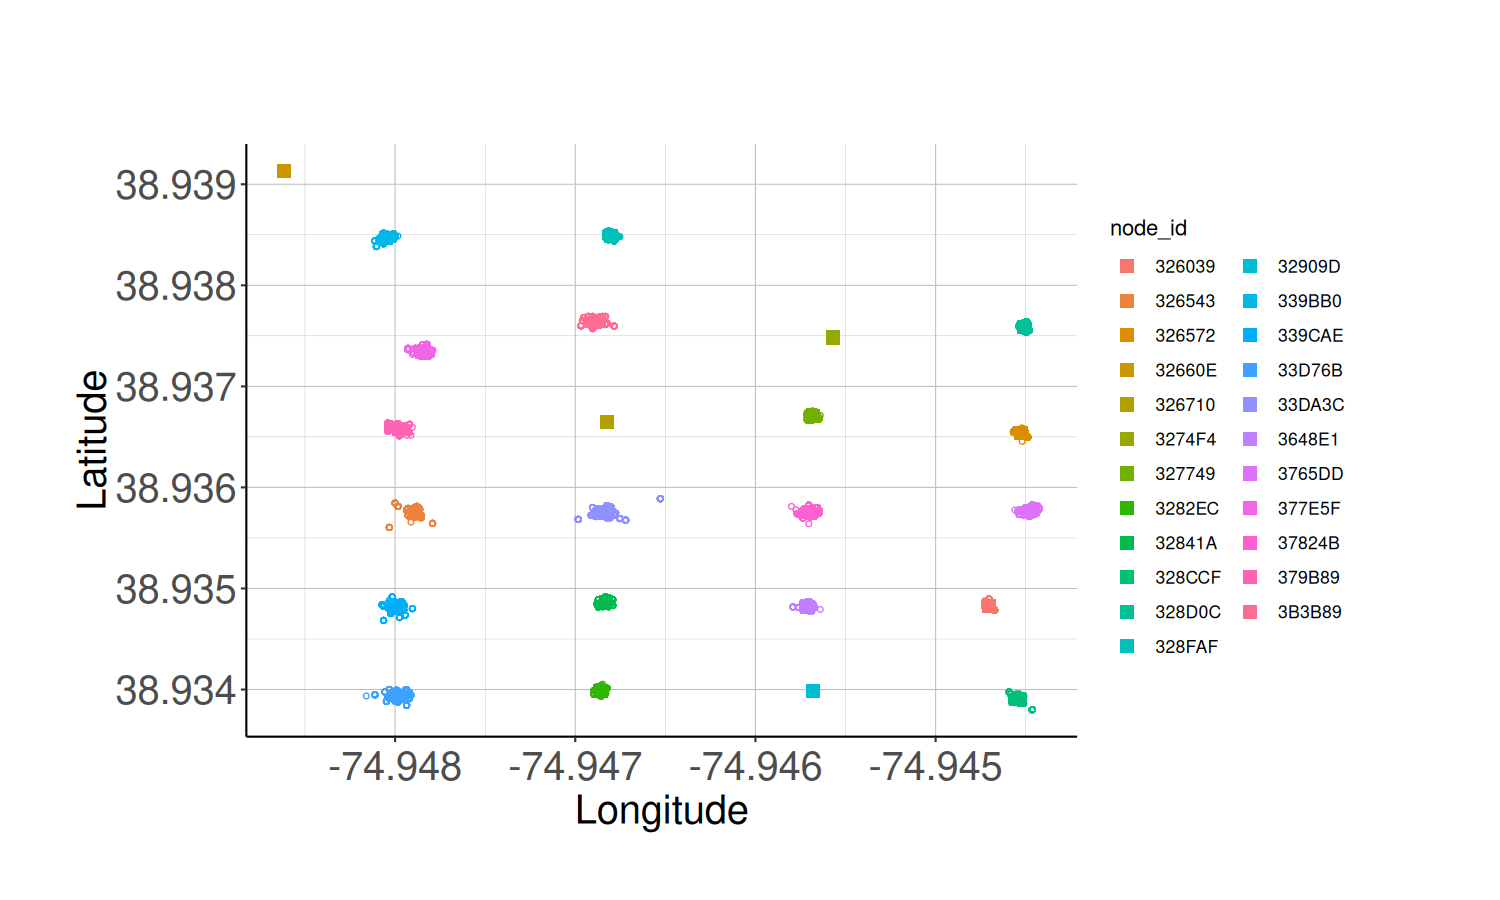
\includegraphics{images/node_calibration_2.4_node_loc_plot.png}
\caption{Node location plot}
\end{figure}

\begin{Shaded}
\begin{Highlighting}[]
\CommentTok{\# Write the node locations to a file}
\FunctionTok{create\_outpath}\NormalTok{(}\StringTok{\textquotesingle{}results\textquotesingle{}}\NormalTok{)}

\FunctionTok{export\_node\_locations}\NormalTok{(}\StringTok{"results/node\_locations.csv"}\NormalTok{, }
\NormalTok{                      node\_locs)}

\CommentTok{\# Draw a map with the node locations}
\NormalTok{node\_map }\OtherTok{\textless{}{-}} \FunctionTok{map\_node\_locations}\NormalTok{(node\_locs, }
                               \AttributeTok{tile\_url =}\NormalTok{ my\_tile\_url)}
\NormalTok{node\_map}
\end{Highlighting}
\end{Shaded}

\begin{figure}
\centering
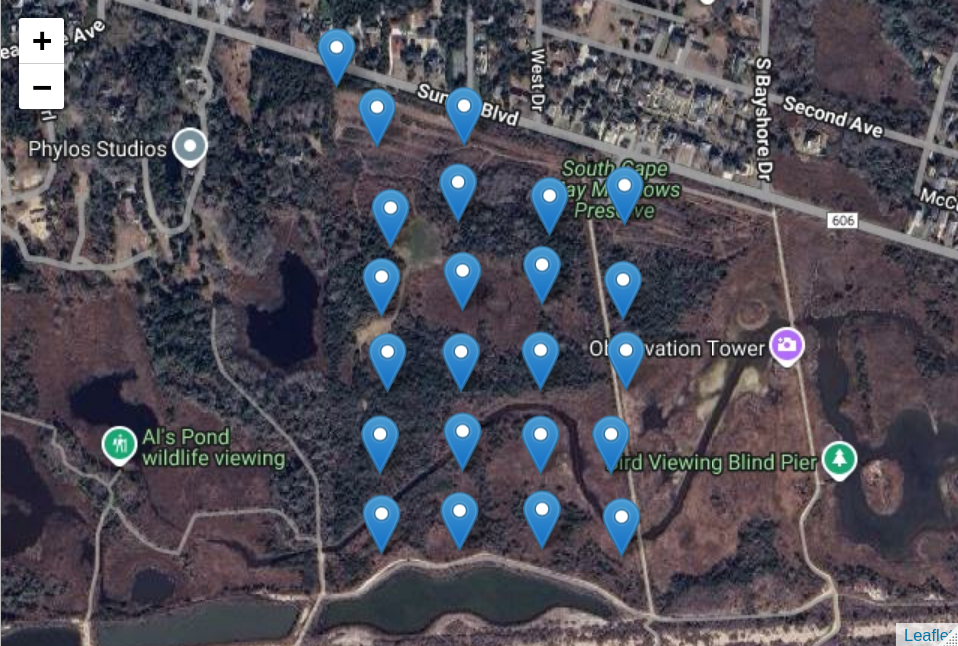
\includegraphics{images/node_calibration_2.4_node_map.png}
\caption{Node location map}
\end{figure}

\subsection{Load Station Detection from Files}\label{load-station-detection-from-files}

\begin{Shaded}
\begin{Highlighting}[]
\CommentTok{\# connect to database}
\NormalTok{con }\OtherTok{\textless{}{-}}\NormalTok{ DBI}\SpecialCharTok{::}\FunctionTok{dbConnect}\NormalTok{(duckdb}\SpecialCharTok{::}\FunctionTok{duckdb}\NormalTok{(), }
                      \AttributeTok{dbdir =}\NormalTok{ database\_file, }
                      \AttributeTok{read\_only =} \ConstantTok{TRUE}\NormalTok{)}

\CommentTok{\# load raw data table and filter from start\_time to stop\_time}
\NormalTok{detection\_df }\OtherTok{\textless{}{-}} \FunctionTok{tbl}\NormalTok{(con, }\StringTok{"raw"}\NormalTok{) }\SpecialCharTok{|\textgreater{}} 
  \FunctionTok{filter}\NormalTok{(time }\SpecialCharTok{\textgreater{}=}\NormalTok{ start\_time }\SpecialCharTok{\&\&}\NormalTok{ time }\SpecialCharTok{\textless{}=}\NormalTok{ stop\_time) }\SpecialCharTok{|\textgreater{}}
  \FunctionTok{collect}\NormalTok{()}

\CommentTok{\# if you are working with blu data, uncomment the lines below and load data from the blu table}
\CommentTok{\# detection\_blu \textless{}{-} tbl(con, "blu") |\textgreater{}}
\CommentTok{\#   filter(time \textgreater{}= start\_time \&\& time \textless{}= stop\_time) |\textgreater{}}
\CommentTok{\#   collect}

\CommentTok{\# disconnect from database}
\NormalTok{DBI}\SpecialCharTok{::}\FunctionTok{dbDisconnect}\NormalTok{(con)}

\CommentTok{\# Get beeps from test tag only}
\NormalTok{detection\_df }\OtherTok{\textless{}{-}} \FunctionTok{subset.data.frame}\NormalTok{(detection\_df, }
\NormalTok{                                  tag\_id }\SpecialCharTok{==}\NormalTok{ my\_tag\_id)}
\end{Highlighting}
\end{Shaded}

\subsection{Load Sidekick Calibration Data}\label{load-sidekick-calibration-data}

\begin{Shaded}
\begin{Highlighting}[]
\CommentTok{\# Get Sidekick data from CSV}
\NormalTok{sidekick\_all\_df }\OtherTok{\textless{}{-}} \FunctionTok{load\_sidekick\_data}\NormalTok{(sidekick\_file\_path)}

\CommentTok{\# Get beeps from test tag only}
\NormalTok{sidekick\_tag\_df }\OtherTok{\textless{}{-}} \FunctionTok{subset.data.frame}\NormalTok{(sidekick\_all\_df, }
\NormalTok{                                     tag\_id }\SpecialCharTok{==}\NormalTok{ my\_tag\_id)}

\CommentTok{\# Show location of all beeps in relation to node locations}
\NormalTok{calibration\_map }\OtherTok{\textless{}{-}} \FunctionTok{map\_calibration\_track}\NormalTok{(node\_locs, }
\NormalTok{                                         sidekick\_tag\_df, }
                                         \AttributeTok{tile\_url =}\NormalTok{ my\_tile\_url)}

\NormalTok{calibration\_map}
\end{Highlighting}
\end{Shaded}

\begin{figure}
\centering
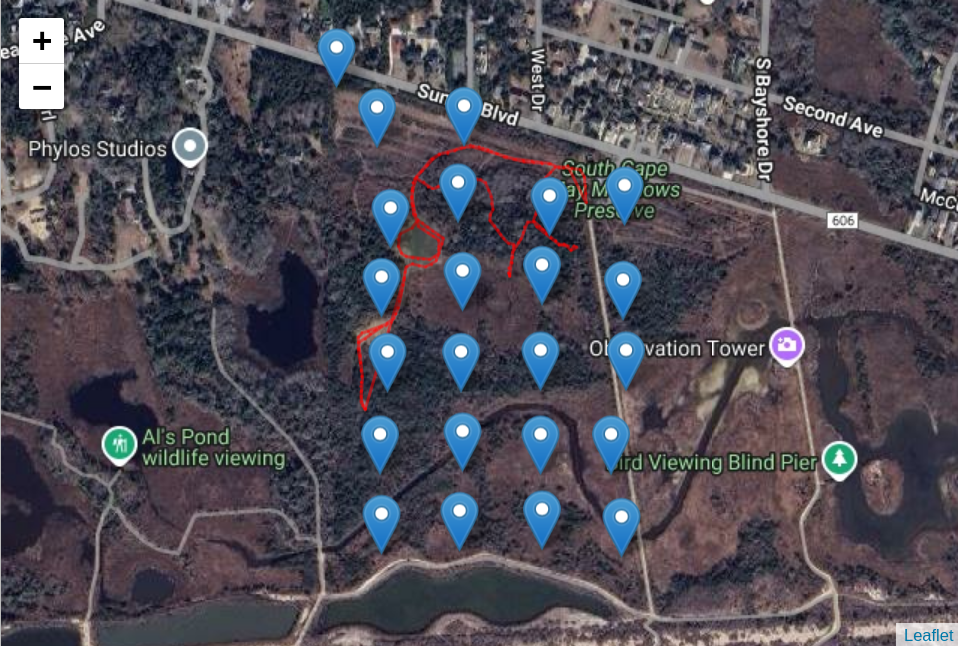
\includegraphics{images/node_calibration_2.5_sidekick_calibration.png}
\caption{Node location plot}
\end{figure}

\section{Calculate the RSSI vs.~Distance Relationship}\label{calculate-the-rssi-vs.-distance-relationship}

This function will match sidekick detections to detections recorded by nodes and sent to the station. Then using the sidekick location, the node locations calculated above, and the rssi measured in the node, a list of rssi and distance pairs is generated and returned.

For Blu Series tags use\_sync=TRUE, for 434 MHz tags use\_sync=FALSE.

\begin{Shaded}
\begin{Highlighting}[]
\NormalTok{rssi\_v\_dist }\OtherTok{\textless{}{-}} \FunctionTok{calc\_rssi\_v\_dist}\NormalTok{(}\AttributeTok{node\_locs =}\NormalTok{ node\_locs, }
                                \AttributeTok{sidekick\_tag\_df =}\NormalTok{ sidekick\_tag\_df, }
                                \AttributeTok{detection\_df =}\NormalTok{ detection\_df, }
                                \AttributeTok{use\_sync =} \ConstantTok{FALSE}\NormalTok{)}

\CommentTok{\# Plot the resulting RSSI and distance data}
\FunctionTok{ggplot}\NormalTok{() }\SpecialCharTok{+}
  \FunctionTok{geom\_point}\NormalTok{(}\AttributeTok{data =}\NormalTok{ rssi\_v\_dist, }
             \FunctionTok{aes}\NormalTok{(}\AttributeTok{x =}\NormalTok{ distance, }
                 \AttributeTok{y =}\NormalTok{ rssi, }
                 \AttributeTok{colour =}\NormalTok{ node\_id)) }\SpecialCharTok{+}
  \FunctionTok{labs}\NormalTok{(}\AttributeTok{title=}\StringTok{"RSSI vs. Distance"}\NormalTok{,}
       \AttributeTok{x=}\StringTok{"Distance (m)"}\NormalTok{,}
       \AttributeTok{y=}\StringTok{"RSSI (dBm)"}\NormalTok{,}
       \AttributeTok{colour=}\StringTok{"Node ID"}\NormalTok{) }\SpecialCharTok{+}
  \FunctionTok{classic\_plot\_theme}\NormalTok{()}
\end{Highlighting}
\end{Shaded}

\begin{figure}
\centering
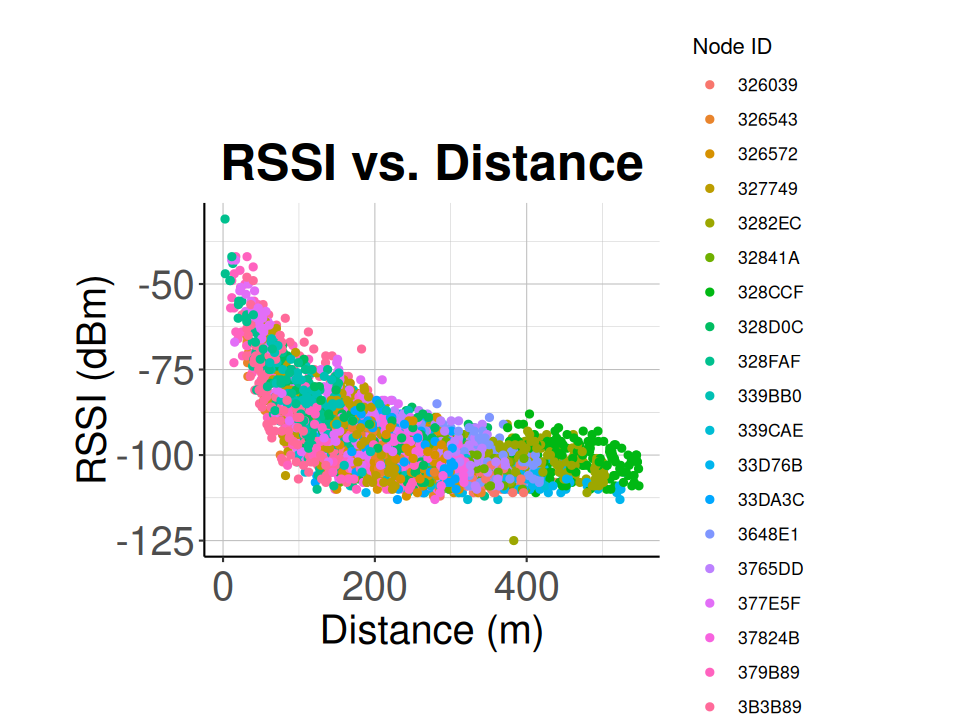
\includegraphics{images/node_calibration_3.1_calculate_rssi_vs_distance.png}
\caption{RSSI vs.~Distance}
\end{figure}

\begin{Shaded}
\begin{Highlighting}[]
\CommentTok{\# Fit the RSSI vs distance data with exponential relationship}
\NormalTok{nlsfit }\OtherTok{\textless{}{-}} \FunctionTok{nls}\NormalTok{(}
\NormalTok{  rssi }\SpecialCharTok{\textasciitilde{}}\NormalTok{ a }\SpecialCharTok{{-}}\NormalTok{ b }\SpecialCharTok{*} \FunctionTok{exp}\NormalTok{(}\SpecialCharTok{{-}}\NormalTok{c }\SpecialCharTok{*}\NormalTok{ distance),}
\NormalTok{  rssi\_v\_dist,}
  \AttributeTok{start =} \FunctionTok{list}\NormalTok{(}\AttributeTok{a =} \SpecialCharTok{{-}}\DecValTok{105}\NormalTok{, }\AttributeTok{b =} \SpecialCharTok{{-}}\DecValTok{60}\NormalTok{, }\AttributeTok{c =} \FloatTok{0.17}\NormalTok{)}
\NormalTok{)}

\FunctionTok{summary}\NormalTok{(nlsfit)}

\CommentTok{\# Get the coefficients from the fit result}
\NormalTok{co }\OtherTok{\textless{}{-}} \FunctionTok{coef}\NormalTok{(}\FunctionTok{summary}\NormalTok{(nlsfit))}
\NormalTok{rssi\_coefs }\OtherTok{\textless{}{-}} \FunctionTok{c}\NormalTok{(co[}\DecValTok{1}\NormalTok{, }\DecValTok{1}\NormalTok{], co[}\DecValTok{2}\NormalTok{, }\DecValTok{1}\NormalTok{], co[}\DecValTok{3}\NormalTok{, }\DecValTok{1}\NormalTok{])}

\CommentTok{\# Add a predicted column to the RSSI vs distance data}
\NormalTok{rssi\_v\_dist}\SpecialCharTok{$}\NormalTok{pred }\OtherTok{\textless{}{-}} \FunctionTok{predict}\NormalTok{(nlsfit)}

\CommentTok{\# Plot the RSSI vs distance data with the fit curve}
\NormalTok{calibration\_plot }\OtherTok{\textless{}{-}} \FunctionTok{plot\_calibration\_result}\NormalTok{(rssi\_v\_dist, }\FunctionTok{classic\_plot\_theme}\NormalTok{())}
\NormalTok{calibration\_plot}

\CommentTok{\# Print the coefficients from the fit. You\textquotesingle{}ll need these coefficients later}
\CommentTok{\# for localization.}
\FunctionTok{print}\NormalTok{(rssi\_coefs)}
\end{Highlighting}
\end{Shaded}

\begin{figure}
\centering
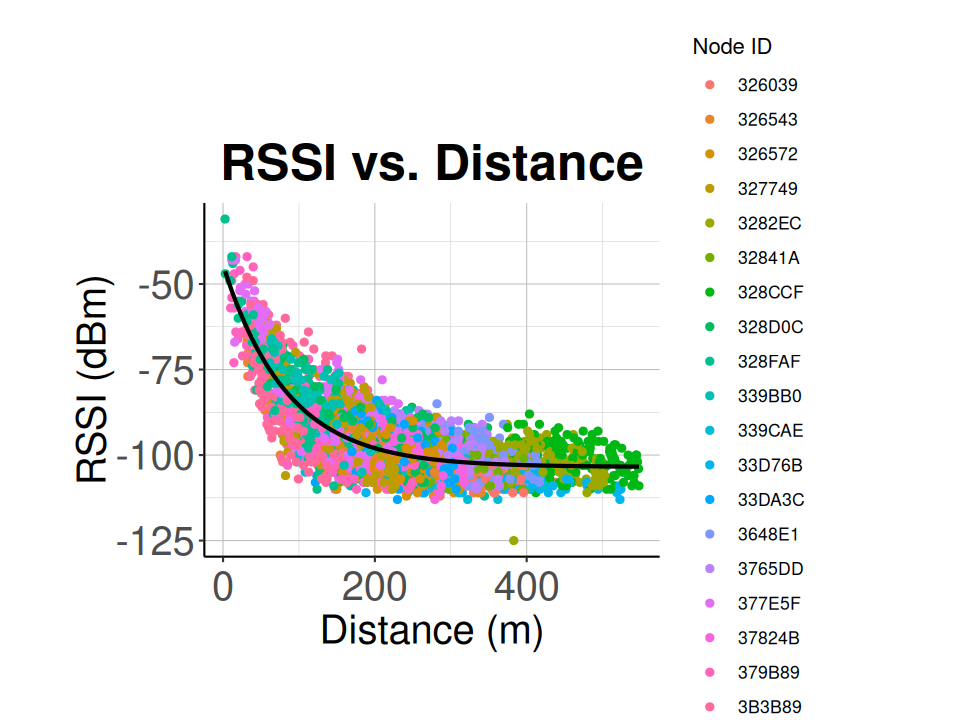
\includegraphics{images/node_calibration_3.1_fit_relationship.png}
\caption{RSSI vs.~Distance}
\end{figure}

Your node grid is now calibrated!

\chapter{Presence/Absence Analysis}\label{presenceabsence-analysis}

This type of analysis can be used to answer questions on stopover duration or for threat monitoring at airports, windmills, etc.

You will need to manually create a tag deployment csv file. This file will contain:
* the tag id (all uppercase)
* the tag deployment date
* the standardized 4-letter Alpha code (if your study involves birds)
* the tag type (Power, Life, Blu)
* the antenna type (1/8 wave)
* any other characteristics of the individual wearing the tag (sex, weight, etc.).

Ex.

\begin{longtable}[]{@{}lllll@{}}
\toprule\noalign{}
TagId & DeployDate & Species & TagType & AntennaType \\
\midrule\noalign{}
\endhead
\bottomrule\noalign{}
\endlastfoot
332D074B & 09/03/23 & NOWA & Power & 1/8 wave \\
664C5219 & 08/23/23 & NOWA & Power & 1/8 wave \\
4C2A0707 & 08/20/23 & NOWA & Power & 1/8 wave \\
\end{longtable}

Then move that tag deployment file into the `outpath' folder.

The \texttt{celltracktech} package includes the deployments data for the Meadows V2 project. We will import it into the RStudio environment and save it as a .csv file in the \texttt{data/Meadows\ V2/} folder for this tutorial.

\begin{Shaded}
\begin{Highlighting}[]
\FunctionTok{write\_csv}\NormalTok{(celltracktech}\SpecialCharTok{::}\NormalTok{deployments, }\StringTok{\textquotesingle{}./data/Meadows V2/meadows\_deployments\_2023.csv\textquotesingle{}}\NormalTok{)}
\end{Highlighting}
\end{Shaded}

If you are using your own data, move your project-specific deployments .csv file into your \texttt{data/\textless{}project\ name\textgreater{}/} folder.

We are now ready to start calculating presence/absence.

\section{Set parameters}\label{set-parameters}

\begin{Shaded}
\begin{Highlighting}[]
\FunctionTok{options}\NormalTok{(}\AttributeTok{digits =} \DecValTok{10}\NormalTok{)}

\CommentTok{\# Specify the path to your database file}
\NormalTok{database\_file }\OtherTok{\textless{}{-}} \StringTok{"./data/Meadows V2/meadows.duckdb"}

\CommentTok{\# Specify the path to the deployment info file}
\NormalTok{deployment\_info\_file }\OtherTok{\textless{}{-}} \StringTok{"data/Meadows V2/meadows\_deployments\_2023.csv"}

\CommentTok{\# Specify the time range of node data you want to import for this analysis}
\NormalTok{start\_time }\OtherTok{\textless{}{-}} \FunctionTok{as.POSIXct}\NormalTok{(}\StringTok{"2023{-}08{-}01 00:00:00"}\NormalTok{, }\AttributeTok{tz =} \StringTok{"GMT"}\NormalTok{)}
\NormalTok{stop\_time }\OtherTok{\textless{}{-}} \FunctionTok{as.POSIXct}\NormalTok{(}\StringTok{"2023{-}12{-}31 00:00:00"}\NormalTok{, }\AttributeTok{tz =} \StringTok{"GMT"}\NormalTok{)}
\end{Highlighting}
\end{Shaded}

\section{Load data from database}\label{load-data-from-database-1}

\begin{Shaded}
\begin{Highlighting}[]
\CommentTok{\# Load from DB}
\NormalTok{con }\OtherTok{\textless{}{-}}\NormalTok{ DBI}\SpecialCharTok{::}\FunctionTok{dbConnect}\NormalTok{(duckdb}\SpecialCharTok{::}\FunctionTok{duckdb}\NormalTok{(), }
                      \AttributeTok{dbdir =}\NormalTok{ database\_file, }
                      \AttributeTok{read\_only =} \ConstantTok{TRUE}\NormalTok{)}

\CommentTok{\# load the raw data table in to RStudio and subset it based on your start and stop times}
\NormalTok{detection\_df }\OtherTok{\textless{}{-}} \FunctionTok{tbl}\NormalTok{(con, }\StringTok{"raw"}\NormalTok{) }\SpecialCharTok{|\textgreater{}} 
  \FunctionTok{filter}\NormalTok{(time }\SpecialCharTok{\textgreater{}=}\NormalTok{ start\_time }\SpecialCharTok{\&}\NormalTok{ time }\SpecialCharTok{\textless{}=}\NormalTok{ stop\_time) }\SpecialCharTok{|\textgreater{}}
  \FunctionTok{collect}\NormalTok{()}

\CommentTok{\# if you study uses blu tags, load the blu data table into RStudio}
\CommentTok{\# detection\_blu \textless{}{-} tbl(con, "blu") |\textgreater{} }
\CommentTok{\#   filter(time \textgreater{}= start\_time \& time \textless{}= stop\_time) |\textgreater{}}
\CommentTok{\#   collect()}

\CommentTok{\# disconnect from database}
\NormalTok{DBI}\SpecialCharTok{::}\FunctionTok{dbDisconnect}\NormalTok{(con)}
\end{Highlighting}
\end{Shaded}

\section{Load Tag Deployment Info}\label{load-tag-deployment-info}

\subsection{Load Tag Deployment File}\label{load-tag-deployment-file}

Again, you will need to create this file yourself. You might want to include other info about the individuals in this file for later analysis (species, weight, sex, etc.).

\begin{Shaded}
\begin{Highlighting}[]
\NormalTok{deployment\_df }\OtherTok{\textless{}{-}} \FunctionTok{read\_csv}\NormalTok{(deployment\_info\_file)}
\end{Highlighting}
\end{Shaded}

\subsection{Get List of Detected Tags}\label{get-list-of-detected-tags}

\begin{Shaded}
\begin{Highlighting}[]
\CommentTok{\# count the number of detections for each tag. the minimum number of detections to be included in this dataframe is 250000. You can set the \textasciigrave{}min\_det\_count\textasciigrave{} to whatever is appropriate for your study.}
\NormalTok{tag\_det\_count }\OtherTok{\textless{}{-}} \FunctionTok{get\_tag\_detection\_count}\NormalTok{(detection\_df, }\AttributeTok{min\_det\_count =} \DecValTok{250000}\NormalTok{)}

\CommentTok{\# plot the number of detections for each individual tag}
\FunctionTok{ggplot}\NormalTok{(tag\_det\_count, }
       \FunctionTok{aes}\NormalTok{(}\AttributeTok{x =} \FunctionTok{factor}\NormalTok{(}\AttributeTok{x =}\NormalTok{ tag\_id,}
                      \AttributeTok{levels =}\NormalTok{ tag\_id), }
           \AttributeTok{y =}\NormalTok{ n)) }\SpecialCharTok{+}
  \FunctionTok{geom\_bar}\NormalTok{(}\AttributeTok{stat =} \StringTok{"identity"}\NormalTok{) }\SpecialCharTok{+}
  \FunctionTok{coord\_flip}\NormalTok{() }\SpecialCharTok{+}
  \FunctionTok{labs}\NormalTok{(}\AttributeTok{x =} \StringTok{"Tag ID"}\NormalTok{, }
       \AttributeTok{y =} \StringTok{"Detection Count"}\NormalTok{) }\SpecialCharTok{+}
  \FunctionTok{tag\_hist\_plot\_theme}\NormalTok{()}
\end{Highlighting}
\end{Shaded}

\begin{figure}
\centering
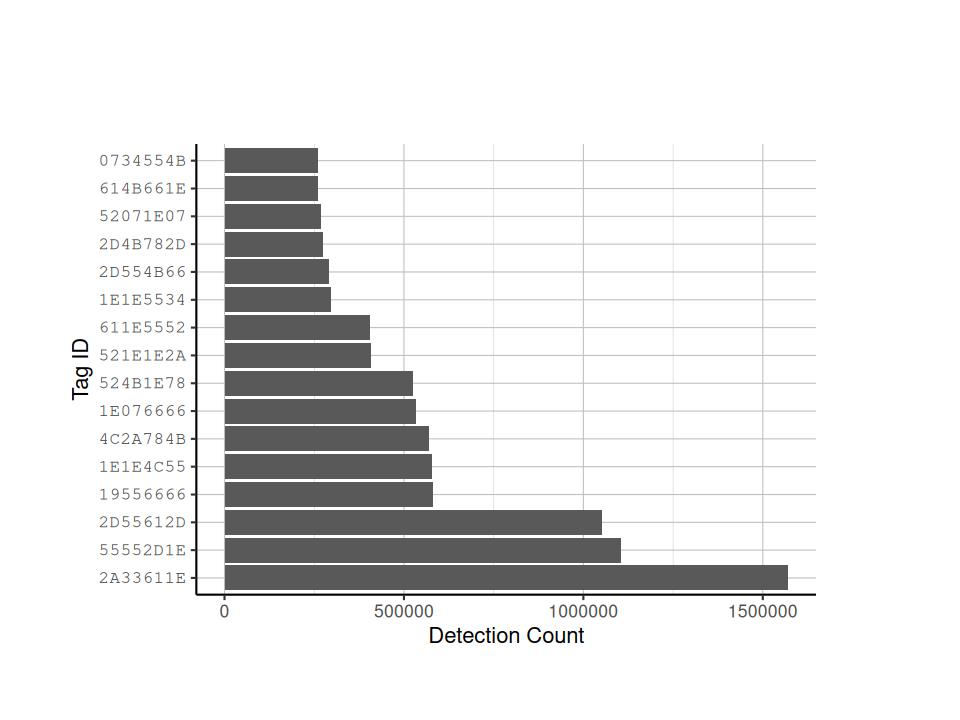
\includegraphics{images/presence_absence_detected_tags_histogram.png}
\caption{Number of detections per tag}
\end{figure}

\section{Generate Detection Summary}\label{generate-detection-summary}

While it is good to know how many detections an individual tag has, it is better to know how many detections there were across time. The code chunk below will subset your \texttt{detection\_df} based on the tags in your tag deployment file, and create a plot of detections across time.

\begin{Shaded}
\begin{Highlighting}[]
\CommentTok{\# Discard detections that aren\textquotesingle{}t from deployed tags}
\NormalTok{detection\_df }\OtherTok{\textless{}{-}} \FunctionTok{subset.data.frame}\NormalTok{(detection\_df, }
\NormalTok{                                  tag\_id }\SpecialCharTok{\%in\%}\NormalTok{ deployment\_df}\SpecialCharTok{$}\NormalTok{TagId) }\SpecialCharTok{|\textgreater{}}
                              \FunctionTok{filter}\NormalTok{(}\FunctionTok{is.na}\NormalTok{(tag\_id) }\SpecialCharTok{==} \ConstantTok{FALSE}\NormalTok{)}

\CommentTok{\# OPTIONAL: You can select individual species here}
\CommentTok{\# subsetting the deployment dataframe to only include NOWA or northern waterthrush}
\NormalTok{deployment\_df }\OtherTok{\textless{}{-}} \FunctionTok{subset.data.frame}\NormalTok{(deployment\_df,}
\NormalTok{                                   Species }\SpecialCharTok{==} \StringTok{"NOWA"}\NormalTok{)}
\CommentTok{\# detection\_df \textless{}{-} subset.data.frame(detection\_df,TagId \%in\% deployment\_df$TagId)}

\NormalTok{det\_summary\_df }\OtherTok{\textless{}{-}} \FunctionTok{detection\_summary}\NormalTok{(}
  \AttributeTok{detection\_df =}\NormalTok{ detection\_df,}
  \AttributeTok{tag\_list =}\NormalTok{ deployment\_df}\SpecialCharTok{$}\NormalTok{TagId}
\NormalTok{)}

\CommentTok{\# create detection summary data frame and sort it based on last detection date}
\NormalTok{det\_summary\_df }\OtherTok{\textless{}{-}}\NormalTok{ det\_summary\_df[}\FunctionTok{order}\NormalTok{(det\_summary\_df}\SpecialCharTok{$}\NormalTok{last\_det, }\AttributeTok{decreasing =} \ConstantTok{TRUE}\NormalTok{), ]}

\CommentTok{\# create a heat{-}bin plot, with the bins reperesenting time periods, and the color representing the number of detections}
\FunctionTok{ggplot}\NormalTok{(}\AttributeTok{data =}\NormalTok{ detection\_df, }
       \FunctionTok{aes}\NormalTok{(}\AttributeTok{x =}\NormalTok{ time, }
           \AttributeTok{y =} \FunctionTok{factor}\NormalTok{(tag\_id, }
\NormalTok{                      det\_summary\_df}\SpecialCharTok{$}\NormalTok{tag\_id))) }\SpecialCharTok{+}
  \FunctionTok{geom\_bin2d}\NormalTok{(}\AttributeTok{binwidth =} \FunctionTok{c}\NormalTok{(}\DecValTok{3600}\NormalTok{, }\DecValTok{1}\NormalTok{)) }\SpecialCharTok{+} \CommentTok{\# Hour time bins}
  \FunctionTok{scale\_fill\_continuous}\NormalTok{(}\AttributeTok{type =} \StringTok{"viridis"}\NormalTok{) }\SpecialCharTok{+}
  \FunctionTok{labs}\NormalTok{(}\AttributeTok{x =} \StringTok{"Time (UTC)"}\NormalTok{, }
       \AttributeTok{y =} \StringTok{"Tag Id"}\NormalTok{) }\SpecialCharTok{+}
  \FunctionTok{tag\_hist\_plot\_theme}\NormalTok{()}
\end{Highlighting}
\end{Shaded}

\begin{figure}
\centering
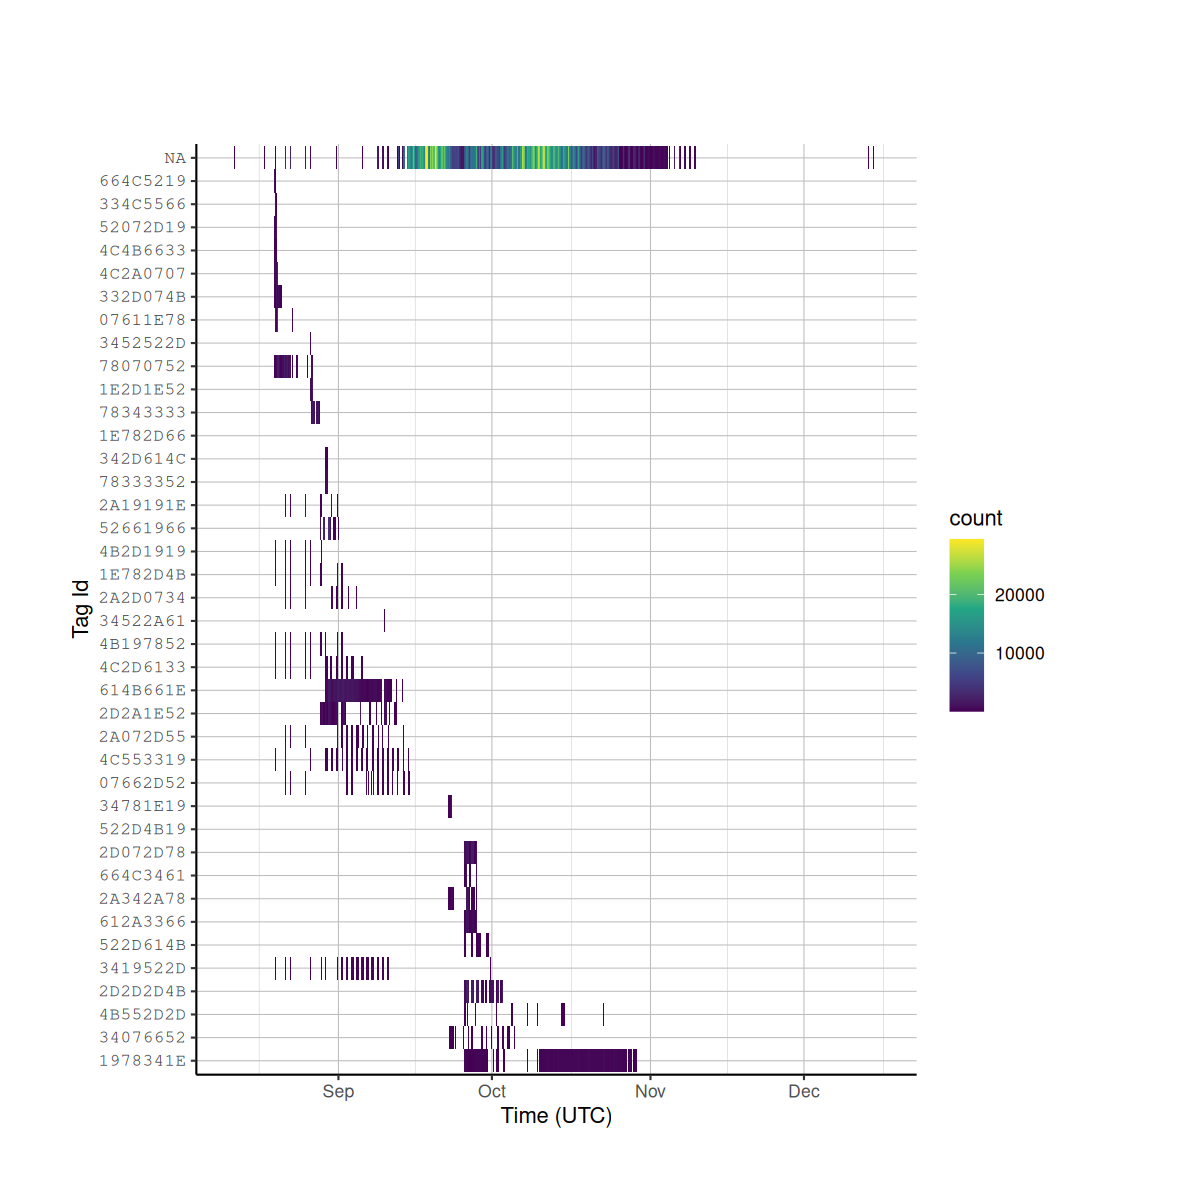
\includegraphics{images/presence_absence_detections_heat_bin.png}
\caption{Heat-plot of tag detections over time}
\end{figure}

\section{Show Detection History for a Specific Tag}\label{show-detection-history-for-a-specific-tag}

\begin{Shaded}
\begin{Highlighting}[]
\CommentTok{\# selected tag is a power tag on a swamp sparrow}
\NormalTok{selected\_tag\_id }\OtherTok{\textless{}{-}} \StringTok{"1978341E"}

\CommentTok{\# set your start and stop times}
\NormalTok{plot\_start\_time }\OtherTok{\textless{}{-}} \FunctionTok{as.POSIXct}\NormalTok{(}\StringTok{"2023{-}10{-}09 10:00:00"}\NormalTok{, }\AttributeTok{tz =} \StringTok{"GMT"}\NormalTok{)}
\NormalTok{plot\_stop\_time }\OtherTok{\textless{}{-}} \FunctionTok{as.POSIXct}\NormalTok{(}\StringTok{"2023{-}10{-}11 14:00:00"}\NormalTok{, }\AttributeTok{tz =} \StringTok{"GMT"}\NormalTok{)}

\CommentTok{\# subset the detection\_df to only include the selected tag id}
\NormalTok{tag\_dets }\OtherTok{\textless{}{-}} \FunctionTok{subset.data.frame}\NormalTok{(detection\_df, tag\_id }\SpecialCharTok{==}\NormalTok{ selected\_tag\_id)}

\CommentTok{\# plot the number of detections for this specific tag at each node across time}
\FunctionTok{ggplot}\NormalTok{(tag\_dets) }\SpecialCharTok{+}
  \FunctionTok{geom\_point}\NormalTok{(}\FunctionTok{aes}\NormalTok{(}\AttributeTok{x =}\NormalTok{ time, }
                 \AttributeTok{y =}\NormalTok{ tag\_rssi, }
                 \AttributeTok{colour =}\NormalTok{ node\_id), }
             \AttributeTok{shape =} \DecValTok{1}\NormalTok{) }\SpecialCharTok{+}
  \FunctionTok{xlim}\NormalTok{(}\FunctionTok{as.POSIXct}\NormalTok{(plot\_start\_time), }
       \FunctionTok{as.POSIXct}\NormalTok{(plot\_stop\_time)) }\SpecialCharTok{+}
  \FunctionTok{ggtitle}\NormalTok{(}\FunctionTok{paste}\NormalTok{(}\StringTok{"Detections"}\NormalTok{, }
\NormalTok{                selected\_tag\_id)) }\SpecialCharTok{+}
  \FunctionTok{xlab}\NormalTok{(}\StringTok{"Time (UTC)"}\NormalTok{) }\SpecialCharTok{+}
  \FunctionTok{ylab}\NormalTok{(}\StringTok{"RSSI (dBm)"}\NormalTok{) }\SpecialCharTok{+}
  \FunctionTok{classic\_plot\_theme}\NormalTok{()}
\end{Highlighting}
\end{Shaded}

\begin{figure}
\centering
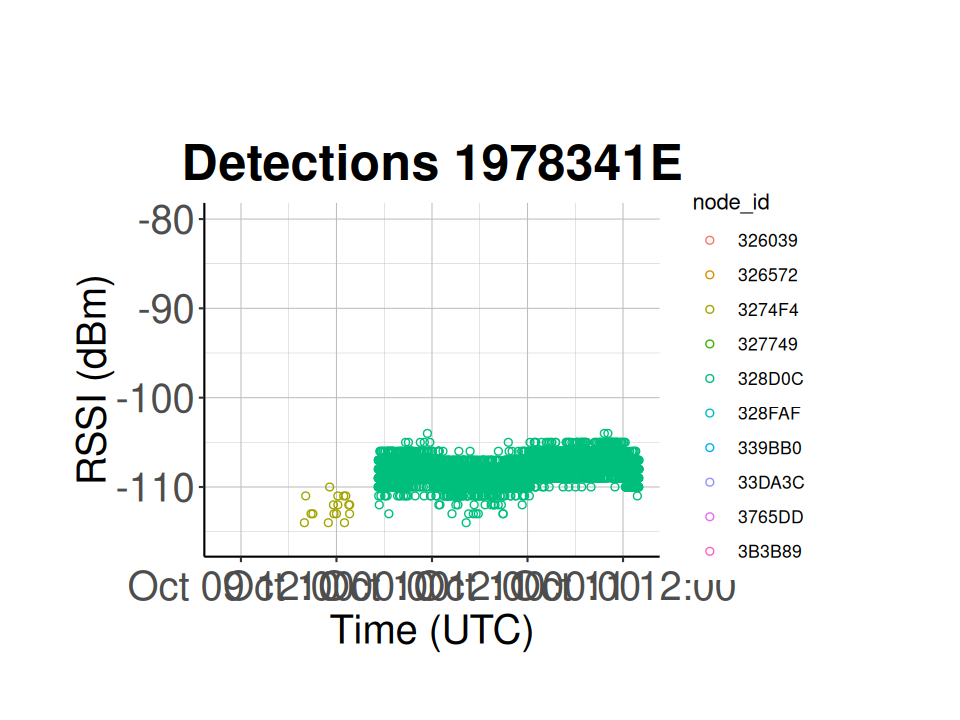
\includegraphics{images/presence_absence_detections_over_time_specific_tag.png}
\caption{Heat-plot of tag detections over time}
\end{figure}

\chapter{Activity Budget}\label{activity-budget}

When is the animal active and/or inactive? Use the following script to answer research questions like:

\begin{itemize}
\tightlist
\item
  Nesting/Incubation behavior
\item
  Roosting times
\item
  Foraging times
\item
  Mortality detection
\end{itemize}

\section{Load settings}\label{load-settings-1}

\begin{Shaded}
\begin{Highlighting}[]
\CommentTok{\# activate renv}
\NormalTok{renv}\SpecialCharTok{::}\FunctionTok{activate}\NormalTok{()}
\end{Highlighting}
\end{Shaded}

\begin{Shaded}
\begin{Highlighting}[]
\CommentTok{\# load celltracktech library}
\FunctionTok{library}\NormalTok{(celltracktech)}

\CommentTok{\# set significant digits}
\FunctionTok{options}\NormalTok{(}\AttributeTok{digits =} \DecValTok{10}\NormalTok{)}

\CommentTok{\# Specify the path to your database file}
\NormalTok{database\_file }\OtherTok{\textless{}{-}} \StringTok{"./data/Meadows V2/meadows.duckdb"}

\NormalTok{start\_time }\OtherTok{\textless{}{-}} \FunctionTok{as.POSIXct}\NormalTok{(}\StringTok{"2023{-}09{-}01 00:00:00"}\NormalTok{,}\AttributeTok{tz =} \StringTok{"GMT"}\NormalTok{)}
\NormalTok{stop\_time }\OtherTok{\textless{}{-}} \FunctionTok{as.POSIXct}\NormalTok{(}\StringTok{"2023{-}09{-}02 00:00:00"}\NormalTok{,}\AttributeTok{tz =} \StringTok{"GMT"}\NormalTok{)}
\end{Highlighting}
\end{Shaded}

\section{Load Tag Node Detection Data}\label{load-tag-node-detection-data}

\begin{Shaded}
\begin{Highlighting}[]
\CommentTok{\# Connect to database}
\NormalTok{con }\OtherTok{\textless{}{-}}\NormalTok{ DBI}\SpecialCharTok{::}\FunctionTok{dbConnect}\NormalTok{(duckdb}\SpecialCharTok{::}\FunctionTok{duckdb}\NormalTok{(), }
                      \AttributeTok{dbdir =}\NormalTok{ database\_file, }
                      \AttributeTok{read\_only =} \ConstantTok{TRUE}\NormalTok{)}

\CommentTok{\# load raw data table into RStudio}
\NormalTok{detection\_df }\OtherTok{\textless{}{-}} \FunctionTok{tbl}\NormalTok{(con, }\StringTok{"raw"}\NormalTok{) }\SpecialCharTok{|\textgreater{}} 
  \FunctionTok{filter}\NormalTok{(time }\SpecialCharTok{\textgreater{}=}\NormalTok{ start\_time }\SpecialCharTok{\&\&}\NormalTok{ time }\SpecialCharTok{\textless{}=}\NormalTok{ stop\_time) }\SpecialCharTok{|\textgreater{}}
  \FunctionTok{collect}\NormalTok{()}

\CommentTok{\# disconnect from the database}
\NormalTok{DBI}\SpecialCharTok{::}\FunctionTok{dbDisconnect}\NormalTok{(con)}
\end{Highlighting}
\end{Shaded}

\section{Tag Activity}\label{tag-activity}

\begin{Shaded}
\begin{Highlighting}[]
\CommentTok{\# selected\_tag\_id \textless{}{-} "2D4B782D", \# SWSP (swamp sparrow) {-} Power Tag}

\CommentTok{\# select a specific tag, below is a Power Tag on a Northern Waterthrush (NOWA)}
\NormalTok{selected\_tag\_id }\OtherTok{\textless{}{-}} \StringTok{\textquotesingle{}614B661E\textquotesingle{}}

\CommentTok{\# subset detection\_df dataframe to only included the selected\_tag\_id}
\NormalTok{tag\_dets }\OtherTok{\textless{}{-}} \FunctionTok{subset.data.frame}\NormalTok{(detection\_df, tag\_id }\SpecialCharTok{==}\NormalTok{ selected\_tag\_id)}

\CommentTok{\# sort the rows by time, ascending}
\NormalTok{tag\_dets }\OtherTok{\textless{}{-}}\NormalTok{ tag\_dets[}\FunctionTok{order}\NormalTok{(tag\_dets}\SpecialCharTok{$}\NormalTok{time, }\AttributeTok{decreasing =} \ConstantTok{FALSE}\NormalTok{), ]}

\NormalTok{tag\_beep\_interval }\OtherTok{\textless{}{-}} \DecValTok{13} \CommentTok{\# seconds, will need to know of tag type beep intervals}

\CommentTok{\# calculate tag activity {-} this turns the number of detections into a single value for a 5 min bin for each Node}
\NormalTok{tag\_activity }\OtherTok{\textless{}{-}} \FunctionTok{calculate\_tag\_activity}\NormalTok{(tag\_dets, tag\_beep\_interval)}

\CommentTok{\# calculate average tag activity}
\NormalTok{avg\_tag\_act }\OtherTok{\textless{}{-}} \FunctionTok{calc\_avg\_activity}\NormalTok{(tag\_activity, start\_time, stop\_time)}

\CommentTok{\# set start and stop times for the plots (next section)}
\NormalTok{plot\_start\_time }\OtherTok{\textless{}{-}} \FunctionTok{as.POSIXct}\NormalTok{(}\StringTok{"2023{-}09{-}01 06:00:00"}\NormalTok{, }\AttributeTok{tz =} \StringTok{"GMT"}\NormalTok{)}
\NormalTok{plot\_stop\_time }\OtherTok{\textless{}{-}} \FunctionTok{as.POSIXct}\NormalTok{(}\StringTok{"2023{-}09{-}02 06:00:00"}\NormalTok{, }\AttributeTok{tz =} \StringTok{"GMT"}\NormalTok{)}
\end{Highlighting}
\end{Shaded}

\subsection{Scatter Plot of RSSI vs time by Node}\label{scatter-plot-of-rssi-vs-time-by-node}

\begin{Shaded}
\begin{Highlighting}[]
\FunctionTok{ggplot}\NormalTok{(}\AttributeTok{data =}\NormalTok{ tag\_dets) }\SpecialCharTok{+}
  \FunctionTok{geom\_point}\NormalTok{(}\FunctionTok{aes}\NormalTok{(}\AttributeTok{x =}\NormalTok{ time, }
                 \AttributeTok{y =}\NormalTok{ tag\_rssi, }
                 \AttributeTok{colour =}\NormalTok{ node\_id), }
             \AttributeTok{shape=}\DecValTok{1}\NormalTok{) }\SpecialCharTok{+}
  \FunctionTok{xlim}\NormalTok{(plot\_start\_time, plot\_stop\_time) }\SpecialCharTok{+}
  \FunctionTok{ggtitle}\NormalTok{(}\FunctionTok{paste}\NormalTok{(}\StringTok{"Detections"}\NormalTok{, selected\_tag\_id)) }\SpecialCharTok{+}
  \FunctionTok{xlab}\NormalTok{(}\StringTok{"Time (UTC)"}\NormalTok{) }\SpecialCharTok{+} 
  \FunctionTok{ylab}\NormalTok{(}\StringTok{"RSSI (dBm)"}\NormalTok{) }\SpecialCharTok{+}
  \FunctionTok{classic\_plot\_theme}\NormalTok{()}
\end{Highlighting}
\end{Shaded}

\begin{figure}
\centering
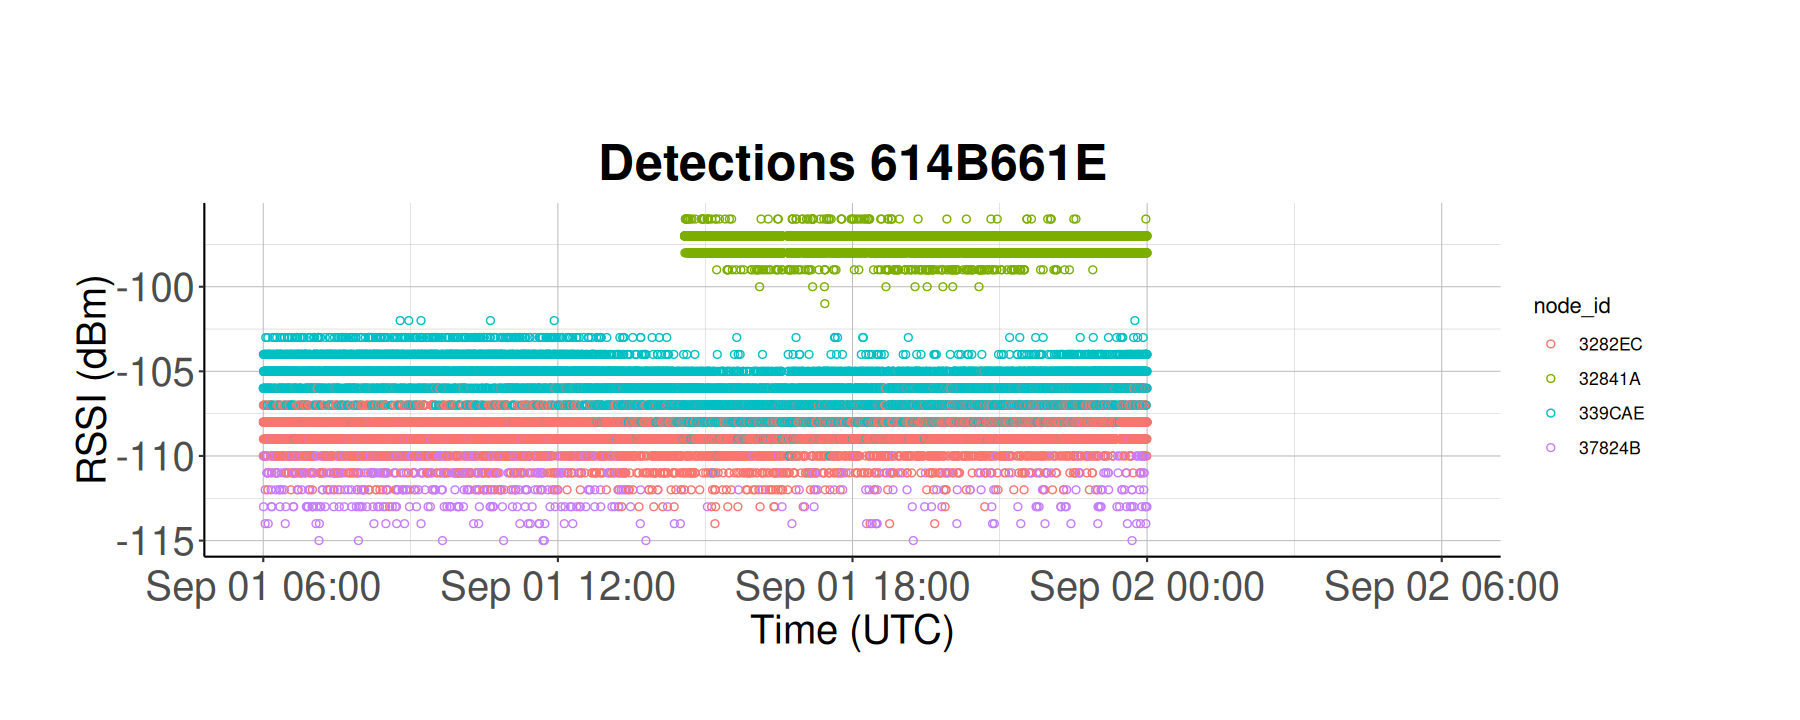
\includegraphics{images/activity_level_rssi_vs_time_by_node.png}
\caption{Scatter plot of RSSI vs time by Node}
\end{figure}

Here we see that this bird was spending most of the time in the vicinity of nodes 3282EC, 339CAE, and 37824B, but the strongest detections are near node 32841A.

\subsection{Scatter Plot of activity vs time by Node}\label{scatter-plot-of-activity-vs-time-by-node}

Next we will quantify the activity level. Activity is an arbitrary variable; it can be movement, roosting, a specific behavior, etc. You will need to define what activity is based on your study.

\begin{Shaded}
\begin{Highlighting}[]
\FunctionTok{ggplot}\NormalTok{(}\AttributeTok{data =}\NormalTok{ tag\_activity) }\SpecialCharTok{+}
  \FunctionTok{geom\_point}\NormalTok{(}\FunctionTok{aes}\NormalTok{(}\AttributeTok{x =}\NormalTok{ time, }
                 \AttributeTok{y =}\NormalTok{ abs\_act, }
                 \AttributeTok{colour =}\NormalTok{ node\_id), }
             \AttributeTok{shape=}\DecValTok{1}\NormalTok{) }\SpecialCharTok{+}
  \FunctionTok{ggtitle}\NormalTok{(}\FunctionTok{paste}\NormalTok{(}\StringTok{"Detections"}\NormalTok{, selected\_tag\_id)) }\SpecialCharTok{+}
  \FunctionTok{xlab}\NormalTok{(}\StringTok{"Time (UTC)"}\NormalTok{) }\SpecialCharTok{+}
  \FunctionTok{ylab}\NormalTok{(}\StringTok{"Activity (Arb. Units)"}\NormalTok{) }\SpecialCharTok{+}
  \FunctionTok{xlim}\NormalTok{(plot\_start\_time, plot\_stop\_time) }\SpecialCharTok{+}
  \FunctionTok{classic\_plot\_theme}\NormalTok{()}
\end{Highlighting}
\end{Shaded}

\begin{figure}
\centering
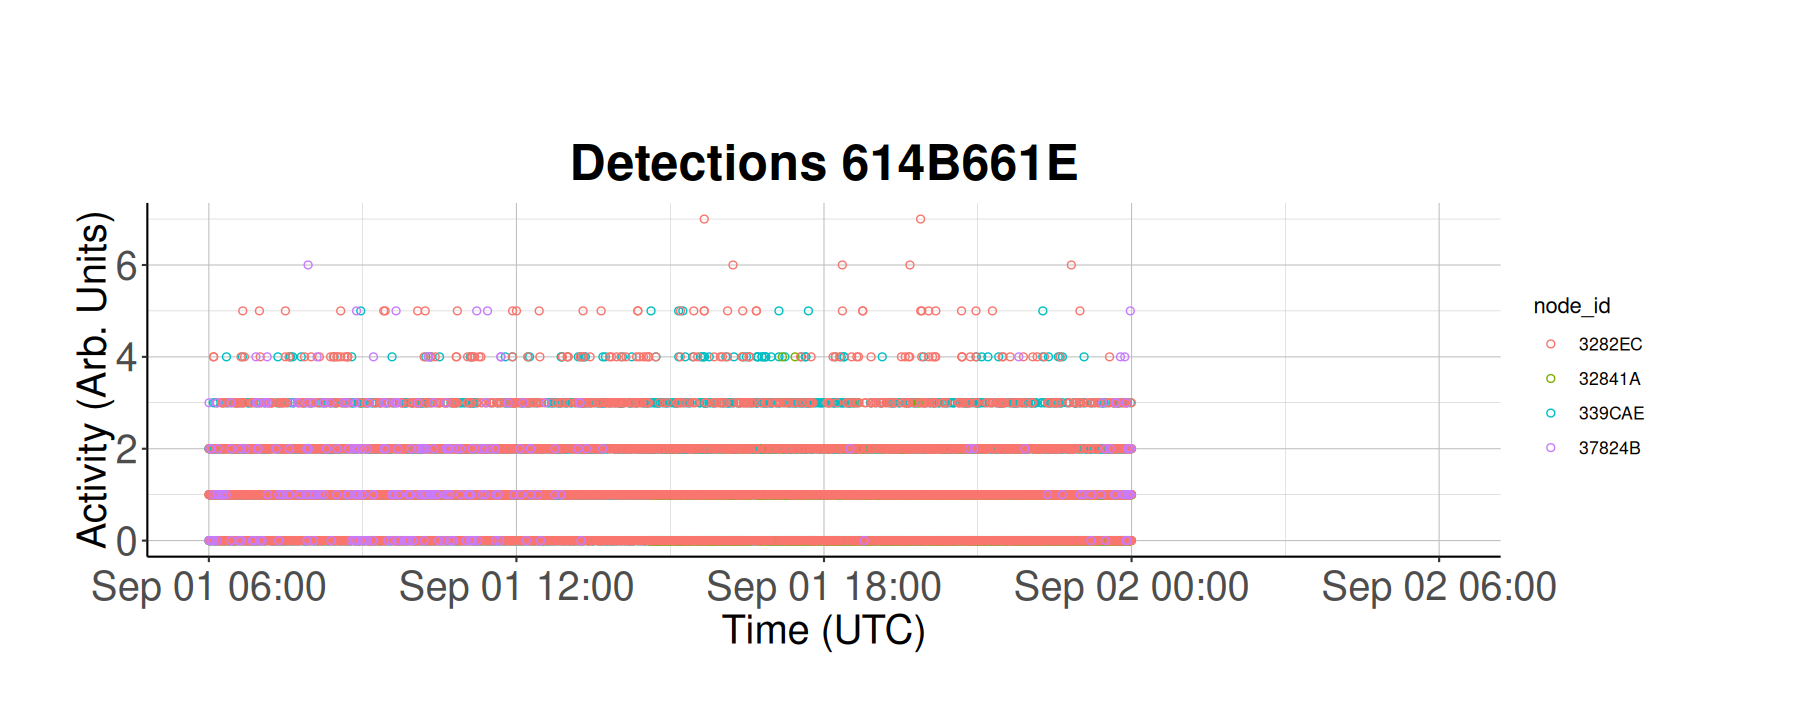
\includegraphics{images/activity_level_activity_vs_time_by_node.png}
\caption{Scatter plot of Activity Level vs time by Node}
\end{figure}

Here we see the activity level (y-axis) for every 5 min from September 1 to September 2. Each color represents a unique Node ID. From a brief glance, this tag had low to mid activity levels near nodes 3282EC and 37824B, but it is still difficult to discern what is going on in this plot.

\subsection{2D Histogram of Activity over Time}\label{d-histogram-of-activity-over-time}

We can summarize the above plot even further by creating a heatmap. The code chunk below creates a heatmap bin plot, which displays the activity for an individual over a period of time, with the color of each bin representing the count of activity (on a log scale), while the bins tell us the activity level.

\begin{Shaded}
\begin{Highlighting}[]
\NormalTok{my\_breaks }\OtherTok{\textless{}{-}} \FunctionTok{c}\NormalTok{(}\DecValTok{1}\NormalTok{, }\DecValTok{10}\NormalTok{, }\DecValTok{100}\NormalTok{, }\DecValTok{1000}\NormalTok{, }\DecValTok{10000}\NormalTok{)}

\FunctionTok{ggplot}\NormalTok{(}\AttributeTok{data =}\NormalTok{ tag\_activity, }
       \FunctionTok{aes}\NormalTok{(}\AttributeTok{x =}\NormalTok{ time, }
           \AttributeTok{y =}\NormalTok{ abs\_act)) }\SpecialCharTok{+}
  \FunctionTok{geom\_bin2d}\NormalTok{(}\AttributeTok{binwidth =} \FunctionTok{c}\NormalTok{(}\DecValTok{3600}\NormalTok{, }\DecValTok{1}\NormalTok{)) }\SpecialCharTok{+}
  \FunctionTok{xlim}\NormalTok{(plot\_start\_time, }
\NormalTok{       plot\_stop\_time) }\SpecialCharTok{+}
  \FunctionTok{scale\_fill\_viridis\_c}\NormalTok{(}\AttributeTok{name =} \StringTok{"Counts"}\NormalTok{, }
                       \AttributeTok{trans =} \StringTok{"log"}\NormalTok{, }
                       \AttributeTok{breaks =}\NormalTok{ my\_breaks, }
                       \AttributeTok{labels =}\NormalTok{ my\_breaks) }\SpecialCharTok{+}
  \FunctionTok{xlab}\NormalTok{(}\StringTok{"Time (UTC)"}\NormalTok{) }\SpecialCharTok{+}
  \FunctionTok{ylab}\NormalTok{(}\StringTok{"Activity / Hour (Arb. Units)"}\NormalTok{) }\SpecialCharTok{+}  
  \FunctionTok{classic\_plot\_theme}\NormalTok{()}
\end{Highlighting}
\end{Shaded}

\begin{figure}
\centering
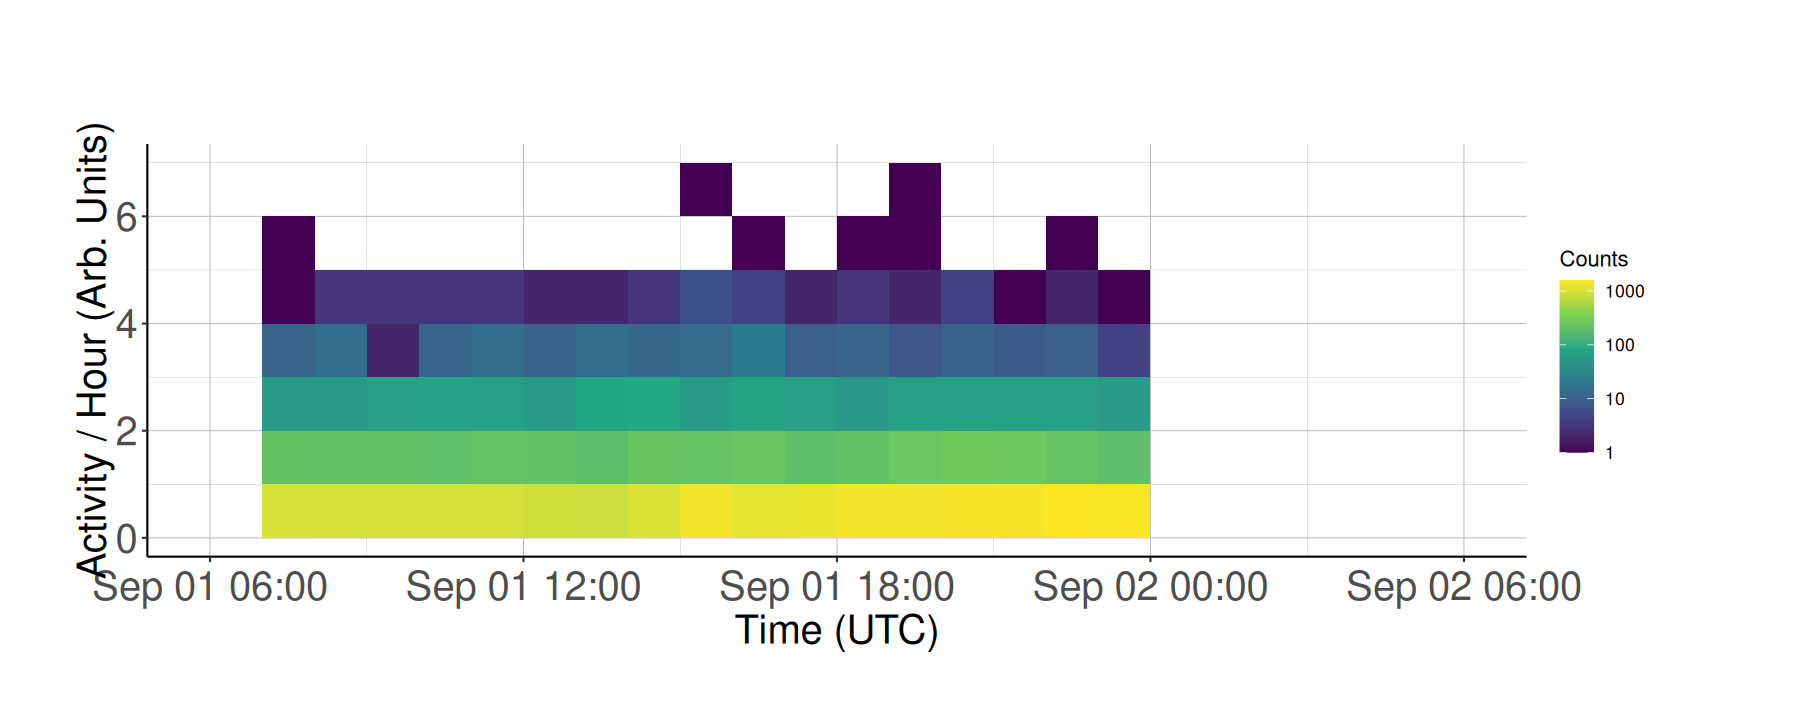
\includegraphics{images/presence_absence_2d_histogram_activity_vs_time.png}
\caption{2D Histogram of Activity over Time by Node}
\end{figure}

From this plot, we can see that there are multiple instances of low activity (demonstrated by the yellow bins at activity/hour 1), and fewer instances of high activity (demonstrated by the blue bins at activity/hour 4 and above).

\subsection{2D histogram of activity vs time WITH avg activity}\label{d-histogram-of-activity-vs-time-with-avg-activity}

This code chunk makes the same plot as above, but also displays the average activity level as a red line.

\begin{Shaded}
\begin{Highlighting}[]
\FunctionTok{ggplot}\NormalTok{(}\AttributeTok{data =}\NormalTok{ tag\_activity, }
       \FunctionTok{aes}\NormalTok{(}\AttributeTok{x =}\NormalTok{ time, }
           \AttributeTok{y =}\NormalTok{ abs\_act)) }\SpecialCharTok{+}
 \FunctionTok{geom\_bin2d}\NormalTok{(}\AttributeTok{binwidth =} \FunctionTok{c}\NormalTok{(}\DecValTok{3600}\NormalTok{, }\DecValTok{1}\NormalTok{)) }\SpecialCharTok{+}
  \FunctionTok{geom\_line}\NormalTok{(}\AttributeTok{data =}\NormalTok{ avg\_tag\_act, }
            \FunctionTok{aes}\NormalTok{(}\AttributeTok{x =}\NormalTok{ time, }
                \AttributeTok{y =}\NormalTok{ avg\_activity),}
            \AttributeTok{colour =} \StringTok{"Red"}\NormalTok{) }\SpecialCharTok{+}
  \FunctionTok{geom\_point}\NormalTok{(}\AttributeTok{data =}\NormalTok{ avg\_tag\_act, }
             \FunctionTok{aes}\NormalTok{(}\AttributeTok{x =}\NormalTok{ time, }
                 \AttributeTok{y =}\NormalTok{ avg\_activity), }
             \AttributeTok{colour =} \StringTok{"Red"}\NormalTok{) }\SpecialCharTok{+}
  \FunctionTok{xlim}\NormalTok{(plot\_start\_time, }
\NormalTok{       plot\_stop\_time) }\SpecialCharTok{+}
  \FunctionTok{xlab}\NormalTok{(}\StringTok{"Time (UTC)"}\NormalTok{) }\SpecialCharTok{+}
  \FunctionTok{ylab}\NormalTok{(}\StringTok{"Activity / Hour (Arb. Units)"}\NormalTok{) }\SpecialCharTok{+}
  \FunctionTok{scale\_fill\_viridis\_c}\NormalTok{(}\AttributeTok{name =} \StringTok{"Counts"}\NormalTok{, }
                       \AttributeTok{trans =} \StringTok{"log"}\NormalTok{, }
                       \AttributeTok{breaks =}\NormalTok{ my\_breaks, }
                       \AttributeTok{labels =}\NormalTok{ my\_breaks) }\SpecialCharTok{+}
  \FunctionTok{classic\_plot\_theme}\NormalTok{()}
\end{Highlighting}
\end{Shaded}

\begin{figure}
\centering
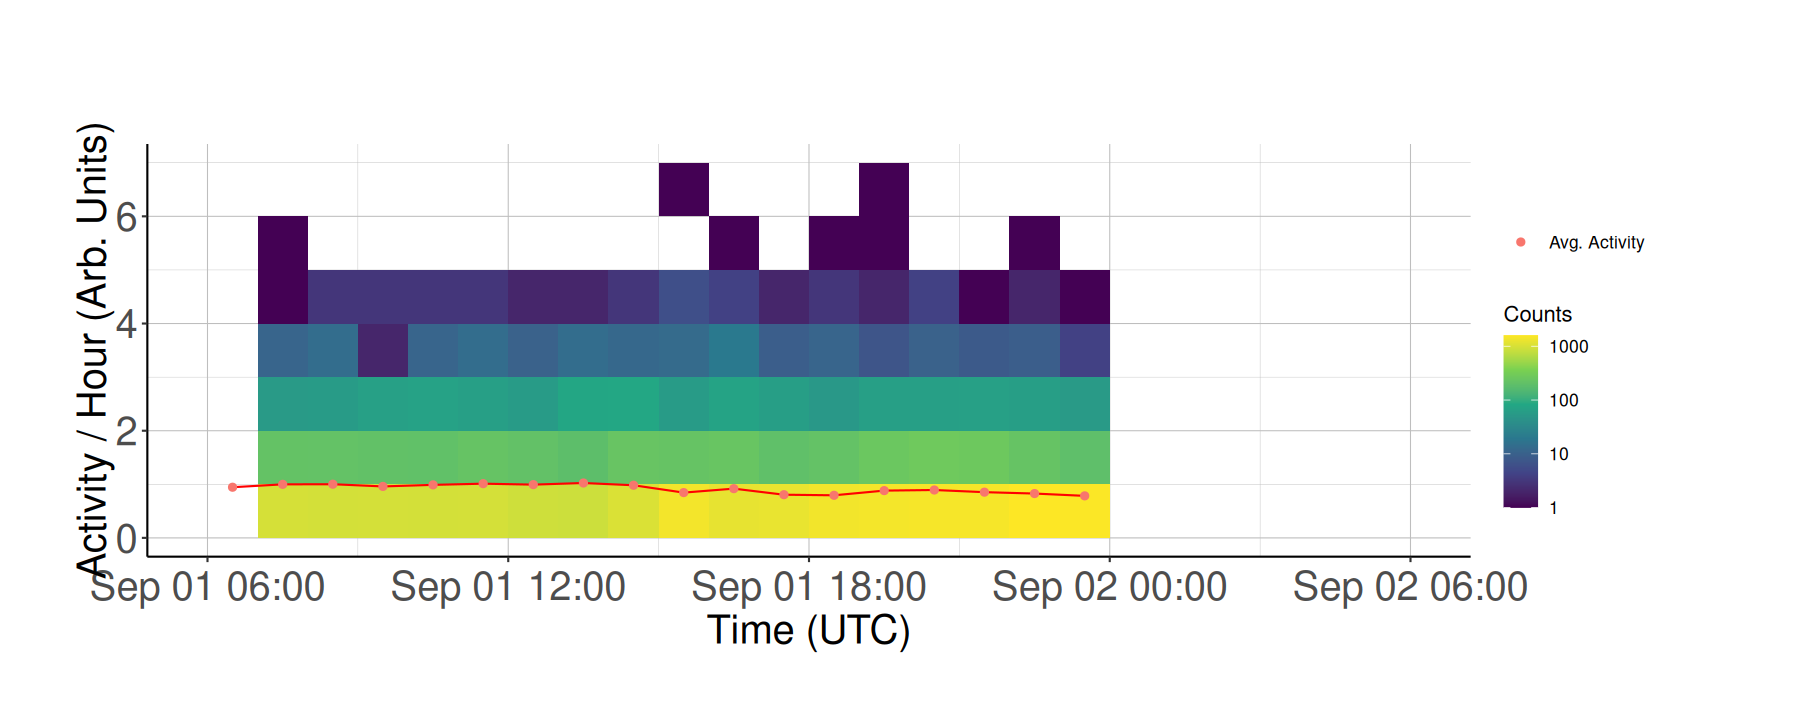
\includegraphics{images/activity_level_average_activity_vs_time.png}
\caption{2D Histogram of Activity over Time by Node with Average Activity}
\end{figure}

Here we see the average activity level for this tag is roughly 1 per hour from September 1 to September 2.

\subsection{Avg activity / hour Vs time.}\label{avg-activity-hour-vs-time.}

Let's zoom in and isolate the average activity per hour:

\begin{Shaded}
\begin{Highlighting}[]
\FunctionTok{ggplot}\NormalTok{(}\AttributeTok{data =}\NormalTok{ tag\_activity) }\SpecialCharTok{+}
  \FunctionTok{geom\_line}\NormalTok{(}\AttributeTok{data =}\NormalTok{ avg\_tag\_act, }
            \FunctionTok{aes}\NormalTok{(}\AttributeTok{x =}\NormalTok{ time, }
                \AttributeTok{y =}\NormalTok{ avg\_activity),}
            \AttributeTok{colour =} \StringTok{"Red"}\NormalTok{) }\SpecialCharTok{+}
  \FunctionTok{geom\_point}\NormalTok{(}\AttributeTok{data =}\NormalTok{ avg\_tag\_act, }
             \FunctionTok{aes}\NormalTok{(}\AttributeTok{x =}\NormalTok{ time, }
                 \AttributeTok{y =}\NormalTok{ avg\_activity), }
             \AttributeTok{colour =} \StringTok{"Red"}\NormalTok{) }\SpecialCharTok{+}
  \FunctionTok{xlim}\NormalTok{(plot\_start\_time, plot\_stop\_time) }\SpecialCharTok{+}
  \FunctionTok{xlab}\NormalTok{(}\StringTok{"Time (UTC)"}\NormalTok{) }\SpecialCharTok{+}
  \FunctionTok{ylab}\NormalTok{(}\StringTok{"Activity / Hour (Arb. Units)"}\NormalTok{) }\SpecialCharTok{+}
  \FunctionTok{scale\_fill\_viridis\_c}\NormalTok{(}\AttributeTok{name =} \StringTok{"Counts"}\NormalTok{, }
                       \AttributeTok{trans =} \StringTok{"log"}\NormalTok{, }
                       \AttributeTok{breaks =}\NormalTok{ my\_breaks, }
                       \AttributeTok{labels =}\NormalTok{ my\_breaks) }\SpecialCharTok{+}
  \FunctionTok{classic\_plot\_theme}\NormalTok{()}
\end{Highlighting}
\end{Shaded}

\begin{figure}
\centering
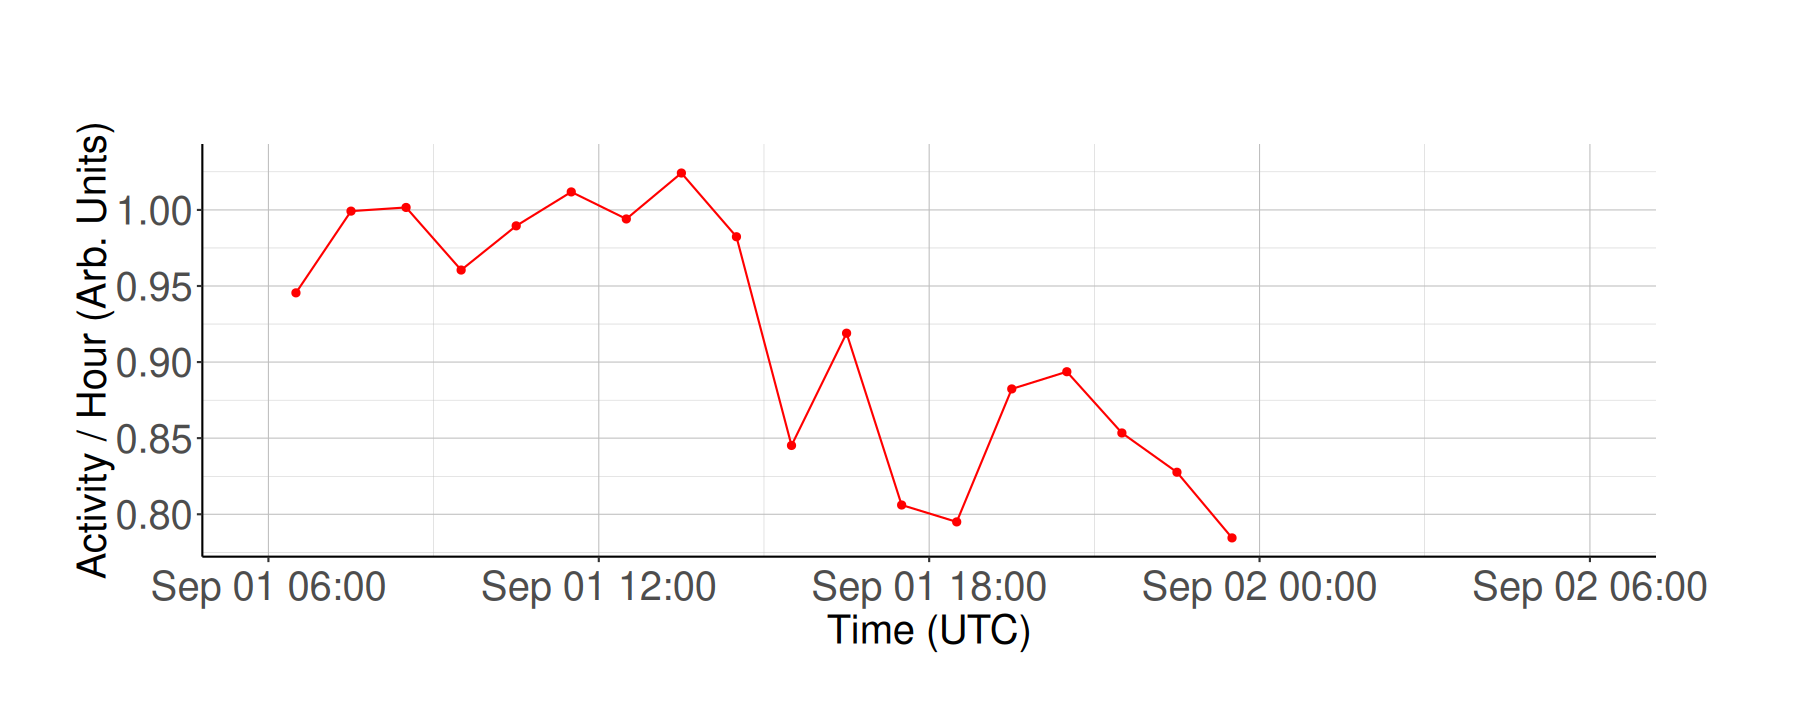
\includegraphics{images/activity_level_average_activity_per_hour_vs_time.png}
\caption{Average Activity per hour vs.~time}
\end{figure}

We see that average activity is highest between 6am-12pm but decreases suddenly after that, which is what we would expect for bird activity level in September.

\chapter{Habitat Use}\label{habitat-use}

Calculate where an animal spends its time.

\section{Load libraries and settings}\label{load-libraries-and-settings}

\subsection{Activate renv}\label{activate-renv}

\begin{Shaded}
\begin{Highlighting}[]
\NormalTok{renv}\SpecialCharTok{::}\FunctionTok{activate}\NormalTok{()}
\end{Highlighting}
\end{Shaded}

\subsection{Load libraries and settings}\label{load-libraries-and-settings-1}

\begin{Shaded}
\begin{Highlighting}[]
\FunctionTok{library}\NormalTok{(celltracktech)}
\end{Highlighting}
\end{Shaded}

\subsection{Load Functions}\label{load-functions}

\begin{Shaded}
\begin{Highlighting}[]
\CommentTok{\# Specify the path to your database file}
\NormalTok{database\_file }\OtherTok{\textless{}{-}} \StringTok{"./data/Meadows V2/meadows.duckdb"}

\CommentTok{\# Specify the path to the deployment info file}
\NormalTok{deployment\_info\_file }\OtherTok{\textless{}{-}} \StringTok{"./data/Meadows V2/meadows\_deployments\_2023.csv"}
\end{Highlighting}
\end{Shaded}

\subsection{Load RSSI Coefficients}\label{load-rssi-coefficients}

Remember Chapter 5 in which we calibrated the node grid? We will want to use those RSSI coefficients to accurately calculate the tag tracks from the detection data.

We will set the coefficients in the code block below, as well as our start and stop time for the Nodes, and for the tag detections.

\begin{Shaded}
\begin{Highlighting}[]
\CommentTok{\# Specify the RSSI vs Distance fit coefficients from calibration}
\NormalTok{a }\OtherTok{\textless{}{-}} \SpecialCharTok{{-}}\FloatTok{103.46373779280}
\NormalTok{b }\OtherTok{\textless{}{-}} \SpecialCharTok{{-}}\FloatTok{59.03199894670}
\NormalTok{c }\OtherTok{\textless{}{-}} \FloatTok{0.01188255653}

\CommentTok{\# create list of rssi coefficients}
\NormalTok{rssi\_coefs }\OtherTok{\textless{}{-}} \FunctionTok{c}\NormalTok{(a, b, c)}
\end{Highlighting}
\end{Shaded}

\subsection{Load Settings}\label{load-settings-2}

\begin{Shaded}
\begin{Highlighting}[]
\FunctionTok{options}\NormalTok{(}\AttributeTok{digits =} \DecValTok{10}\NormalTok{)}

\CommentTok{\# Specify the time range of node data you want to import for this analysis}
\CommentTok{\#   This range should cover a large time window where your nodes were in}
\CommentTok{\#   a constant location.  All node health records in this time window}
\CommentTok{\#   will be used to accurately determine the position of your nodes}
\NormalTok{node\_start\_time }\OtherTok{\textless{}{-}} \FunctionTok{as.POSIXct}\NormalTok{(}\StringTok{"2023{-}08{-}01 00:00:00"}\NormalTok{, }\AttributeTok{tz =} \StringTok{"GMT"}\NormalTok{)}
\NormalTok{node\_stop\_time }\OtherTok{\textless{}{-}} \FunctionTok{as.POSIXct}\NormalTok{(}\StringTok{"2023{-}08{-}07 00:00:00"}\NormalTok{, }\AttributeTok{tz =} \StringTok{"GMT"}\NormalTok{)}

\CommentTok{\# Selected Tag Id {-} Hybrid tag on a Gray Catbird (GRCA)}
\NormalTok{selected\_tag\_id }\OtherTok{\textless{}{-}} \StringTok{\textquotesingle{}2A33611E\textquotesingle{}} \CommentTok{\# tag with most detections, 1/4 wave}

\CommentTok{\# Analysis Time Range}
\NormalTok{det\_start\_time }\OtherTok{\textless{}{-}} \FunctionTok{as.POSIXct}\NormalTok{(}\StringTok{"2023{-}10{-}01 12:00:00"}\NormalTok{, }\AttributeTok{tz =} \StringTok{"GMT"}\NormalTok{)}
\NormalTok{det\_stop\_time }\OtherTok{\textless{}{-}} \FunctionTok{as.POSIXct}\NormalTok{(}\StringTok{"2023{-}10{-}06 12:00:00"}\NormalTok{, }\AttributeTok{tz =} \StringTok{"GMT"}\NormalTok{)}

\CommentTok{\# You can specify an alternative map tile URL to use here}
\NormalTok{my\_tile\_url }\OtherTok{\textless{}{-}} \StringTok{"https://mt2.google.com/vt/lyrs=y\&x=\{x\}\&y=\{y\}\&z=\{z\}"}
\end{Highlighting}
\end{Shaded}

\section{Load Node Health Data from Files}\label{load-node-health-data-from-files-1}

\begin{Shaded}
\begin{Highlighting}[]
\CommentTok{\# Load from DB}
\NormalTok{con }\OtherTok{\textless{}{-}}\NormalTok{ DBI}\SpecialCharTok{::}\FunctionTok{dbConnect}\NormalTok{(duckdb}\SpecialCharTok{::}\FunctionTok{duckdb}\NormalTok{(), }
                      \AttributeTok{dbdir =}\NormalTok{ database\_file, }
                      \AttributeTok{read\_only =} \ConstantTok{TRUE}\NormalTok{)}

\CommentTok{\# load node\_health data table into RStudio and filter it based on the start and stop time}
\NormalTok{node\_health\_df }\OtherTok{\textless{}{-}} \FunctionTok{tbl}\NormalTok{(con, }\StringTok{"node\_health"}\NormalTok{) }\SpecialCharTok{|\textgreater{}}
  \FunctionTok{filter}\NormalTok{(time }\SpecialCharTok{\textgreater{}=}\NormalTok{ node\_start\_time }\SpecialCharTok{\&\&}\NormalTok{ time }\SpecialCharTok{\textless{}=}\NormalTok{ node\_stop\_time) }\SpecialCharTok{|\textgreater{}}
  \FunctionTok{collect}\NormalTok{()}

\CommentTok{\# disconnect from the database}
\NormalTok{DBI}\SpecialCharTok{::}\FunctionTok{dbDisconnect}\NormalTok{(con)}

\CommentTok{\# Remove duplicates}
\NormalTok{node\_health\_df }\OtherTok{\textless{}{-}}\NormalTok{ node\_health\_df }\SpecialCharTok{\%\textgreater{}\%} 
  \FunctionTok{distinct}\NormalTok{(node\_id, }
\NormalTok{           time, }
\NormalTok{           recorded\_at, }
           \AttributeTok{.keep\_all =} \ConstantTok{TRUE}\NormalTok{)}
\end{Highlighting}
\end{Shaded}

\section{Get Node Locations}\label{get-node-locations-1}

Due to variations in GPS coordinates, it is a good idea to plot the Node locations and overlay the plot over a satellite image of your study site.

\begin{Shaded}
\begin{Highlighting}[]
\CommentTok{\# Calculate the average node locations}
\NormalTok{node\_locs }\OtherTok{\textless{}{-}} \FunctionTok{calculate\_node\_locations}\NormalTok{(node\_health\_df)}

\CommentTok{\# Plot the average node locations}
\NormalTok{node\_loc\_plot }\OtherTok{\textless{}{-}} \FunctionTok{plot\_node\_locations}\NormalTok{(node\_health\_df, }
\NormalTok{                                     node\_locs, }
                                     \AttributeTok{theme =} \FunctionTok{classic\_plot\_theme}\NormalTok{())}
\NormalTok{node\_loc\_plot}
\end{Highlighting}
\end{Shaded}

\begin{figure}
\centering
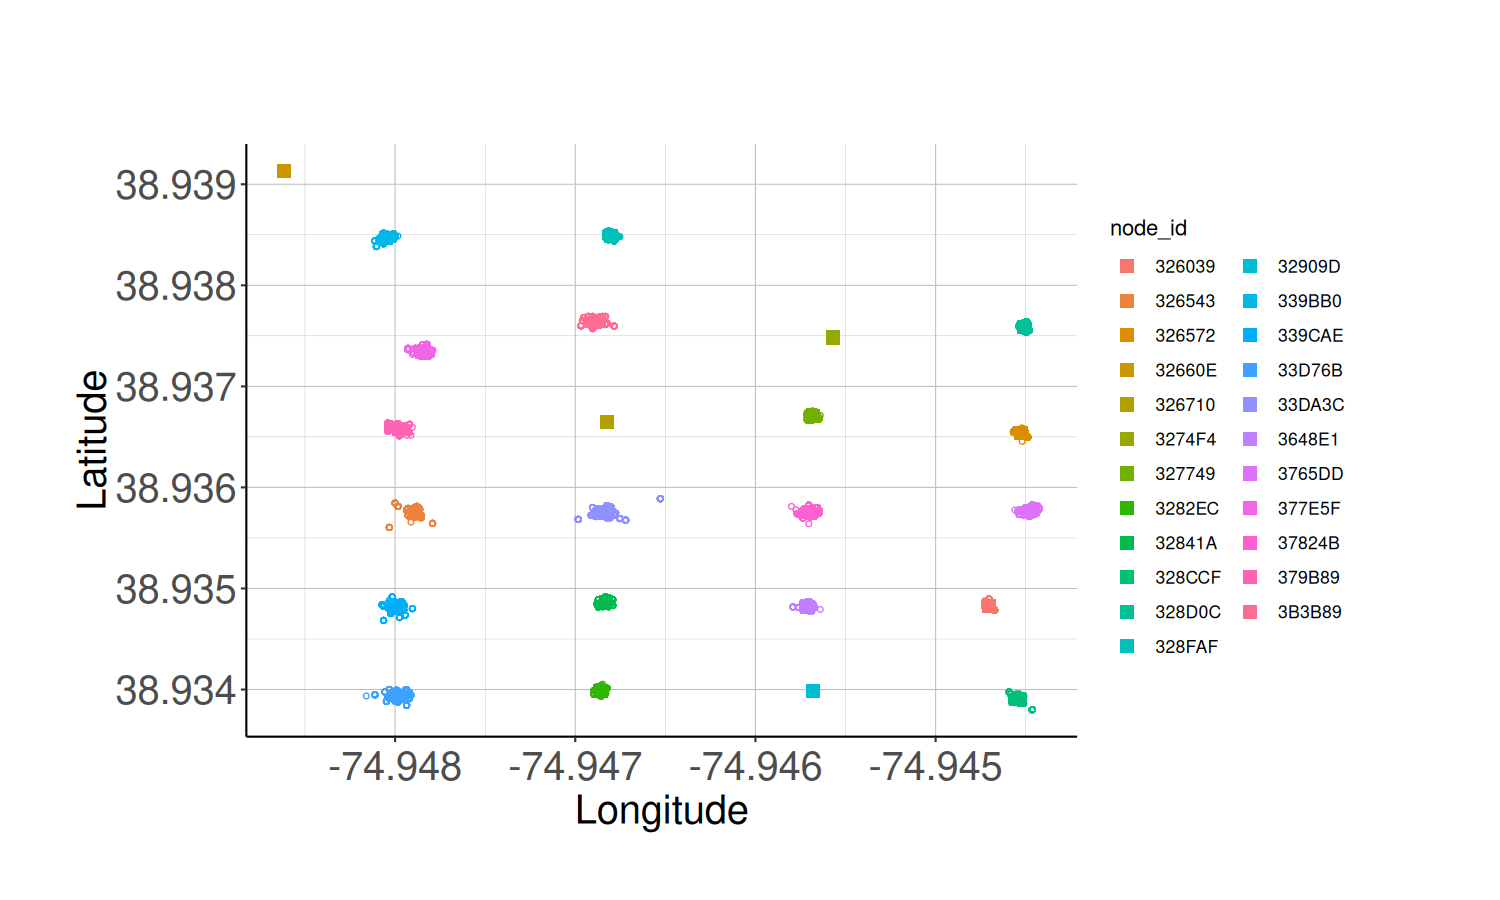
\includegraphics{images/habitat_use_node_loc_plot.png}
\caption{Average node locations}
\end{figure}

\begin{Shaded}
\begin{Highlighting}[]
\CommentTok{\# Draw a map with the node locations}
\NormalTok{node\_map }\OtherTok{\textless{}{-}} \FunctionTok{map\_node\_locations}\NormalTok{(node\_locs, }\AttributeTok{tile\_url =}\NormalTok{ my\_tile\_url)}
\NormalTok{node\_map}
\end{Highlighting}
\end{Shaded}

\begin{figure}
\centering
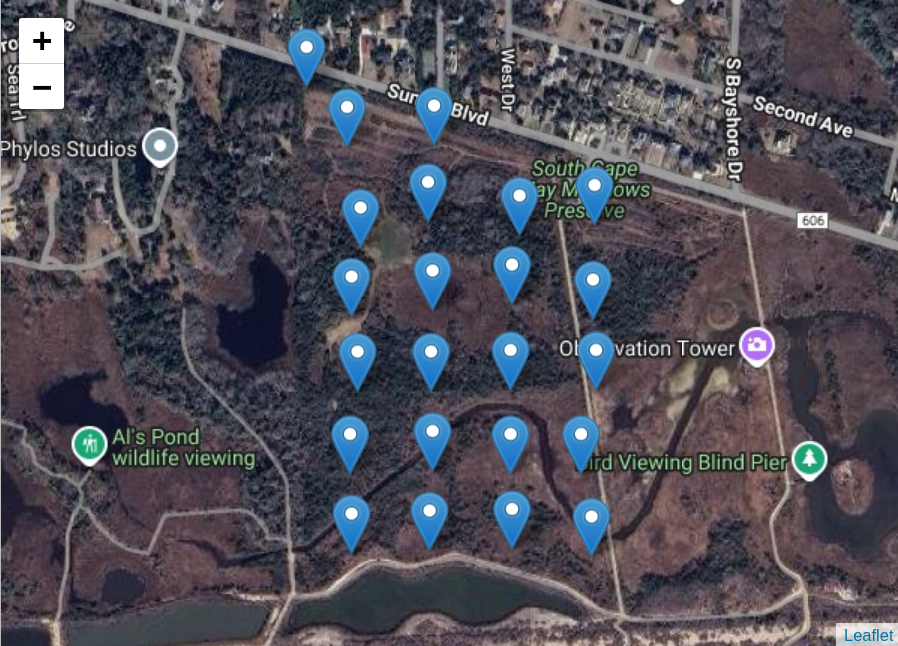
\includegraphics{images/habitat_use_node_map.png}
\caption{Node location map}
\end{figure}

\section{Load Station Detection Data}\label{load-station-detection-data}

These are your tag detections in the `raw' or `blu' data tables in your database.

\begin{Shaded}
\begin{Highlighting}[]
\CommentTok{\# Load from DB}
\NormalTok{con }\OtherTok{\textless{}{-}}\NormalTok{ DBI}\SpecialCharTok{::}\FunctionTok{dbConnect}\NormalTok{(duckdb}\SpecialCharTok{::}\FunctionTok{duckdb}\NormalTok{(), }
                      \AttributeTok{dbdir =}\NormalTok{ database\_file, }
                      \AttributeTok{read\_only =} \ConstantTok{TRUE}\NormalTok{)}

\CommentTok{\# load raw data table into RStudio and filter it based on start and stop time}
\NormalTok{detection\_df }\OtherTok{\textless{}{-}} \FunctionTok{tbl}\NormalTok{(con, }\StringTok{"raw"}\NormalTok{) }\SpecialCharTok{|\textgreater{}}
  \FunctionTok{filter}\NormalTok{(time }\SpecialCharTok{\textgreater{}=}\NormalTok{ det\_start\_time }\SpecialCharTok{\&\&}\NormalTok{ time }\SpecialCharTok{\textless{}=}\NormalTok{ det\_stop\_time) }\SpecialCharTok{|\textgreater{}}
  \FunctionTok{filter}\NormalTok{(tag\_id }\SpecialCharTok{==}\NormalTok{ selected\_tag\_id) }\SpecialCharTok{|\textgreater{}}
  \FunctionTok{collect}\NormalTok{()}

\CommentTok{\# disconnect from the databse}
\NormalTok{DBI}\SpecialCharTok{::}\FunctionTok{dbDisconnect}\NormalTok{(con)}

\CommentTok{\# create time\_value variable}
\NormalTok{detection\_df }\OtherTok{\textless{}{-}}\NormalTok{ detection\_df }\SpecialCharTok{\%\textgreater{}\%} 
  \FunctionTok{mutate}\NormalTok{(}\AttributeTok{time\_value =} \FunctionTok{as.integer}\NormalTok{(time))}
\end{Highlighting}
\end{Shaded}

\section{Build a Grid}\label{build-a-grid}

To actually quantify the amount of habitat an animal uses, we will create a 500x800 m grid and overlay it over the map. Each grid bin will be 5x5m.

\begin{Shaded}
\begin{Highlighting}[]
\CommentTok{\# set the grid coordinates}
\NormalTok{grid\_center\_lat }\OtherTok{\textless{}{-}} \FloatTok{38.93664800}
\NormalTok{grid\_center\_lon }\OtherTok{\textless{}{-}} \SpecialCharTok{{-}}\FloatTok{74.9462}
\NormalTok{grid\_size\_x }\OtherTok{\textless{}{-}} \DecValTok{500} \CommentTok{\# meters}
\NormalTok{grid\_size\_y }\OtherTok{\textless{}{-}} \DecValTok{800} \CommentTok{\# meters}
\NormalTok{grid\_bin\_size }\OtherTok{\textless{}{-}} \DecValTok{5} \CommentTok{\# meters}

\CommentTok{\# Create a data frame with the details about the grid}
\NormalTok{grid\_df }\OtherTok{\textless{}{-}} \FunctionTok{build\_grid}\NormalTok{(}
  \AttributeTok{node\_locs =}\NormalTok{ node\_locs,}
  \AttributeTok{center\_lat =}\NormalTok{ grid\_center\_lat,}
  \AttributeTok{center\_lon =}\NormalTok{ grid\_center\_lon,}
  \AttributeTok{x\_size\_meters =}\NormalTok{ grid\_size\_x,}
  \AttributeTok{y\_size\_meters =}\NormalTok{ grid\_size\_y,}
  \AttributeTok{bin\_size =}\NormalTok{ grid\_bin\_size}
\NormalTok{)}

\CommentTok{\# Draw all of the grid bins on a map}
\NormalTok{grid\_map }\OtherTok{\textless{}{-}} \FunctionTok{draw\_grid}\NormalTok{(node\_locs, grid\_df)}
\NormalTok{grid\_map}
\end{Highlighting}
\end{Shaded}

\begin{figure}
\centering
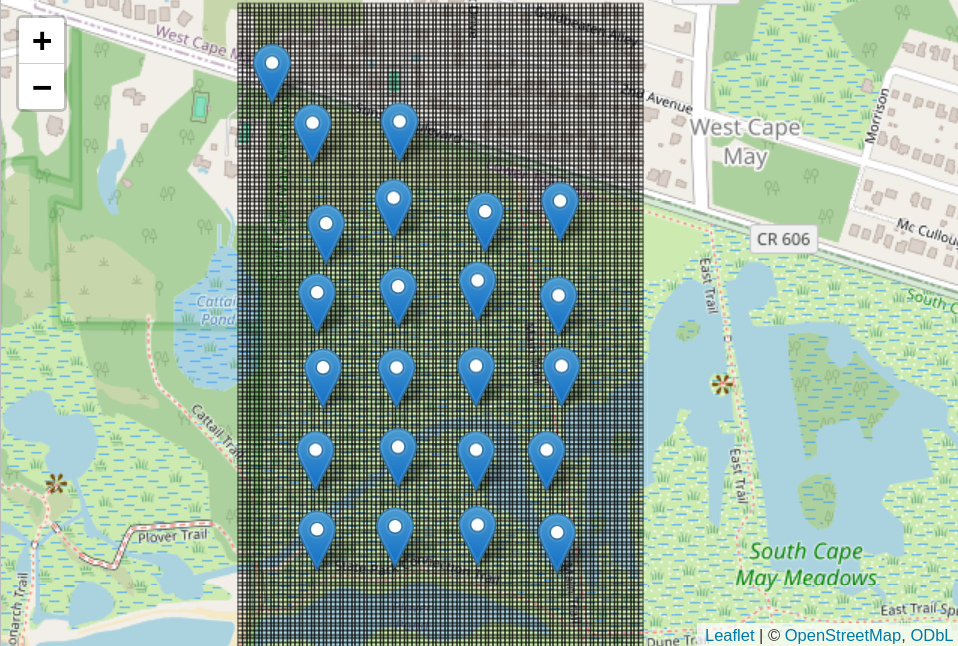
\includegraphics{images/habitat_use_grid_map.png}
\caption{Node grid map}
\end{figure}

\section{Calculate Locations}\label{calculate-locations}

This will display the tag tracks and the tag location on the node grid map.

\begin{Shaded}
\begin{Highlighting}[]
\CommentTok{\# create a locations dataframe with the calculate\_track() function}
\NormalTok{locations\_df }\OtherTok{\textless{}{-}} \FunctionTok{calculate\_track}\NormalTok{(}
  \AttributeTok{start\_time =} \StringTok{"2023{-}10{-}04 23:00:00"}\NormalTok{,}
  \CommentTok{\# start\_time = "2023{-}08{-}01 00:00:00",}
  \AttributeTok{length\_seconds =} \DecValTok{6} \SpecialCharTok{*} \DecValTok{3600}\NormalTok{,}
  \AttributeTok{step\_size\_seconds =} \DecValTok{15}\NormalTok{,}
  \AttributeTok{det\_time\_window =} \DecValTok{30}\NormalTok{, }\CommentTok{\# Must have detection within this window to be included in position calculation}
  \AttributeTok{filter\_alpha =} \FloatTok{0.7}\NormalTok{,}
  \AttributeTok{filter\_time\_range =} \DecValTok{60}\NormalTok{, }\CommentTok{\# Time range to include detections in filtered value}
  \AttributeTok{grid\_df =}\NormalTok{ grid\_df,}
  \AttributeTok{detection\_df =}\NormalTok{ detection\_df,}
  \AttributeTok{node\_locs =}\NormalTok{ node\_locs,}
  \AttributeTok{rssi\_coefs =}\NormalTok{ rssi\_coefs,}
  \AttributeTok{track\_frame\_output\_path =} \ConstantTok{NULL} \CommentTok{\# If NULL no individual frames will be saved}
\NormalTok{)}
\FunctionTok{print}\NormalTok{(locations\_df)}

\CommentTok{\# overlay the tag tracks on the node grid and satelitte picture}
\NormalTok{track\_map }\OtherTok{\textless{}{-}} \FunctionTok{map\_track}\NormalTok{(node\_locs, }
\NormalTok{                       locations\_df, }
\NormalTok{                       my\_tile\_url)}
\NormalTok{track\_map}
\end{Highlighting}
\end{Shaded}

\begin{figure}
\centering
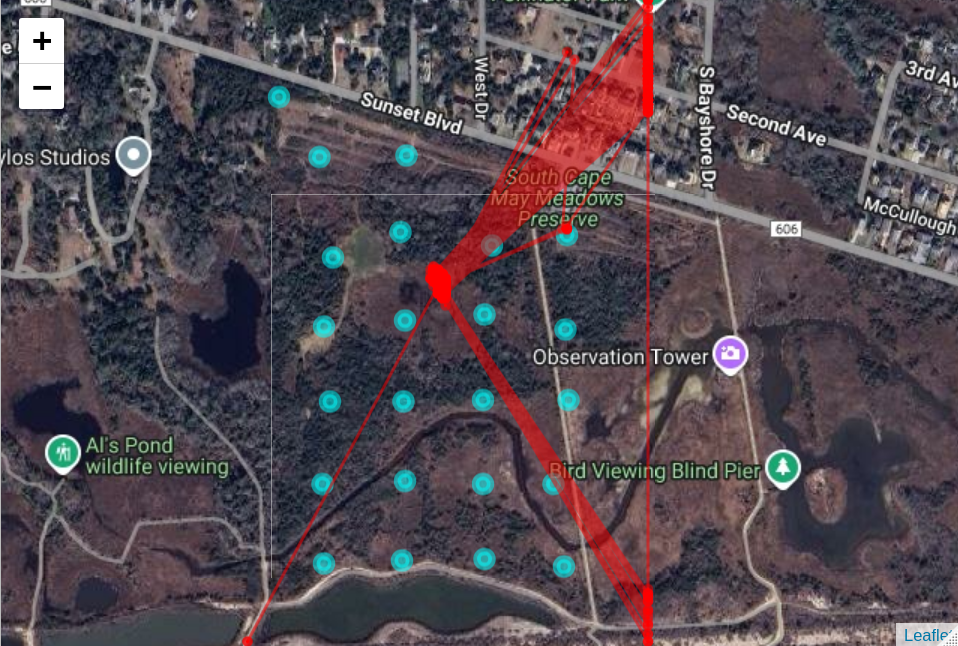
\includegraphics{images/habitat_use_track_map.png}
\caption{Node track map}
\end{figure}

\begin{Shaded}
\begin{Highlighting}[]
\CommentTok{\# calculate and display the location density on the node grid map}
\CommentTok{\# source("R/functions/grid\_search/grid\_search\_functions.R")}
\NormalTok{loc\_density }\OtherTok{\textless{}{-}} \FunctionTok{calc\_location\_density}\NormalTok{(}\AttributeTok{grid\_df =}\NormalTok{ grid\_df, }
                                     \AttributeTok{locations\_df =}\NormalTok{ locations\_df)}

\NormalTok{loc\_density\_map }\OtherTok{\textless{}{-}} \FunctionTok{map\_location\_density}\NormalTok{(}\AttributeTok{loc\_density\_df =}\NormalTok{ loc\_density, my\_tile\_url)}
\NormalTok{loc\_density\_map}
\end{Highlighting}
\end{Shaded}

\begin{figure}
\centering
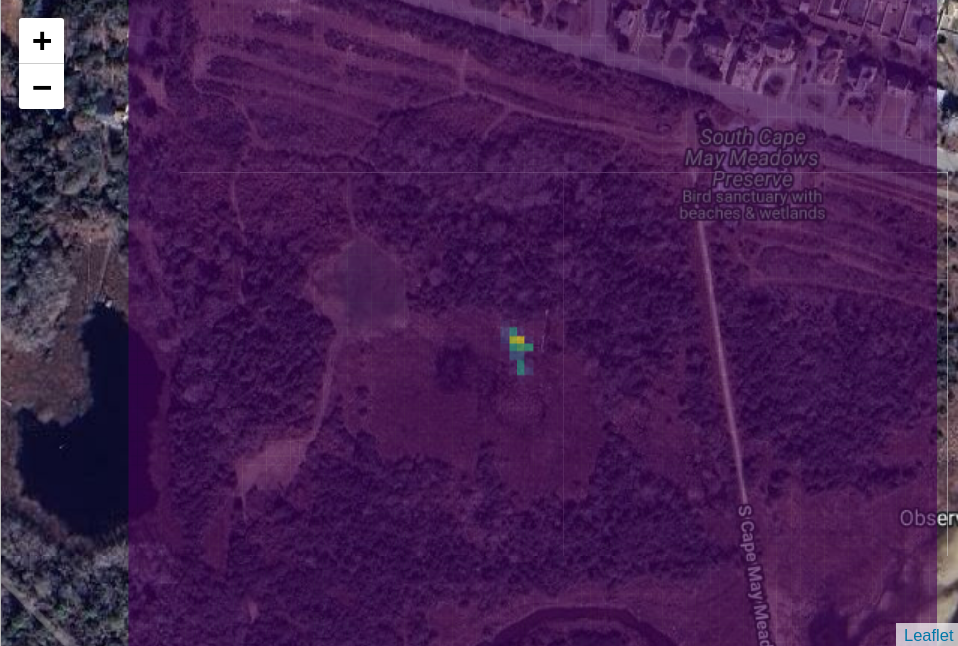
\includegraphics{images/habitat_use_location_density_map.png}
\caption{Location Density Map}
\end{figure}

If you zoom in on the map, you can see the areas where the animal spent most of its time.

For tags with 1/8 wavelengths, you may need to use a lower RSSI coefficient to accurately map tracks and habitat use. Try using -115 for RSSI coefficient `a'.

Below is an example of a Power Tag with a 1/8 wave antenna, and will need a lower RSSI coefficient:

\begin{Shaded}
\begin{Highlighting}[]
\CommentTok{\# Specify the RSSI vs Distance fit coefficients from calibration}
\NormalTok{a }\OtherTok{\textless{}{-}} \SpecialCharTok{{-}}\FloatTok{115.0} \CommentTok{\# for 1/8 wave tags}
\NormalTok{b }\OtherTok{\textless{}{-}} \SpecialCharTok{{-}}\FloatTok{59.03199894670}
\NormalTok{c }\OtherTok{\textless{}{-}} \FloatTok{0.01188255653}

\NormalTok{rssi\_coefs }\OtherTok{\textless{}{-}} \FunctionTok{c}\NormalTok{(a, b, c)}

\CommentTok{\# Selected Tag Id {-} Power Tag on a Swamp Sparrow (SWSP), 1/8 wave}
\NormalTok{selected\_tag\_id }\OtherTok{\textless{}{-}} \StringTok{"2D4B782D"}
\end{Highlighting}
\end{Shaded}

Run the rest of the code blocks after setting these new RSSI coefficients to plot the habitat use of an individual with a 1/8 wave antenna.

\chapter{Grid Search Analysis}\label{grid-search-analysis}

If you are interested in the extent of an animal's movement, use the following grid search analysis.

Like in Chapter 8 - Habitat Use, the grid search analysis divides an area into a grid, and calculates the received signal strength at each node. Then this process is repeated for each time step in a series of detections recorded by the node network.

\section{Loading Settings}\label{loading-settings}

\subsection{Activate renv}\label{activate-renv-1}

\begin{Shaded}
\begin{Highlighting}[]
\NormalTok{renv}\SpecialCharTok{::}\FunctionTok{activate}\NormalTok{()}
\end{Highlighting}
\end{Shaded}

\subsection{Load libraries}\label{load-libraries}

\begin{Shaded}
\begin{Highlighting}[]
\FunctionTok{library}\NormalTok{(celltracktech)}
\end{Highlighting}
\end{Shaded}

\subsection{Load settings}\label{load-settings-3}

\begin{Shaded}
\begin{Highlighting}[]
\CommentTok{\# Specify the path to your database file}
\NormalTok{database\_file }\OtherTok{\textless{}{-}} \StringTok{"./data/Meadows V2/meadows.duckdb"}

\CommentTok{\# (OPTIONAL) Specify Node time offsets if necessary}
\NormalTok{node\_time\_offset\_file }\OtherTok{\textless{}{-}} \StringTok{"./data/Meadows V2/node\_time\_offset\_20230802.csv"}
\NormalTok{node\_toff\_df }\OtherTok{\textless{}{-}} \FunctionTok{read.csv}\NormalTok{(node\_time\_offset\_file)}

\CommentTok{\# Specify the tag ID that you want to locate}
\NormalTok{my\_tag\_id }\OtherTok{\textless{}{-}} \StringTok{"072A6633"}

\CommentTok{\# Specify the RSSI vs Distance fit coefficients from calibration}
\NormalTok{a }\OtherTok{\textless{}{-}} \SpecialCharTok{{-}}\FloatTok{103.0610446987}
\NormalTok{b }\OtherTok{\textless{}{-}} \SpecialCharTok{{-}}\FloatTok{60.6023833206}
\NormalTok{c }\OtherTok{\textless{}{-}} \FloatTok{0.0120558164}
\NormalTok{rssi\_coefs }\OtherTok{\textless{}{-}} \FunctionTok{c}\NormalTok{(a, b, c)}

\CommentTok{\# Specify the time range of node data you want to import for this analysis}
\CommentTok{\#   This range should cover a large time window where your nodes were in}
\CommentTok{\#   a constant location.  All node health records in this time window}
\CommentTok{\#   will be used to accurately determine the position of your nodes}

\CommentTok{\# IMPORTANT! If you have included a node time offset file,}
\CommentTok{\# make sure it was calculated using the same start and stop times as below.}
\NormalTok{node\_start\_time }\OtherTok{\textless{}{-}} \FunctionTok{as.POSIXct}\NormalTok{(}\StringTok{"2023{-}08{-}01 00:00:00"}\NormalTok{, }\AttributeTok{tz =} \StringTok{"GMT"}\NormalTok{)}
\NormalTok{node\_stop\_time }\OtherTok{\textless{}{-}} \FunctionTok{as.POSIXct}\NormalTok{(}\StringTok{"2023{-}08{-}07 00:00:00"}\NormalTok{, }\AttributeTok{tz =} \StringTok{"GMT"}\NormalTok{)}

\CommentTok{\# Specify time range of detection data you want to pull from the DB}
\NormalTok{det\_start\_time }\OtherTok{\textless{}{-}} \FunctionTok{as.POSIXct}\NormalTok{(}\StringTok{"2023{-}08{-}03 00:00:00"}\NormalTok{, }\AttributeTok{tz =} \StringTok{"GMT"}\NormalTok{)}
\NormalTok{det\_stop\_time }\OtherTok{\textless{}{-}} \FunctionTok{as.POSIXct}\NormalTok{(}\StringTok{"2023{-}08{-}04 00:00:00"}\NormalTok{, }\AttributeTok{tz =} \StringTok{"GMT"}\NormalTok{)}

\CommentTok{\# Specify a list of node Ids if you only want to include a subset in calibration}
\CommentTok{\# IF you want to use all nodes, ignore this line and SKIP the step below}
\CommentTok{\# where the data frame is trimmed to only nodes in this list}
\CommentTok{\# my\_nodes \textless{}{-} c("B25AC19E", "44F8E426", "FAB6E12", "1EE02113", "565AA5B9", "EE799439", "1E762CF3", "A837A3F4", "484ED33B")}

\CommentTok{\# You can specify an alternative map tile URL to use here}
\NormalTok{my\_tile\_url }\OtherTok{\textless{}{-}} \StringTok{"https://mt2.google.com/vt/lyrs=y\&x=\{x\}\&y=\{y\}\&z=\{z\}"}
\end{Highlighting}
\end{Shaded}

\section{Load Node Health data from Database}\label{load-node-health-data-from-database}

\begin{Shaded}
\begin{Highlighting}[]
\CommentTok{\# Load from DB}
\NormalTok{con }\OtherTok{\textless{}{-}}\NormalTok{ DBI}\SpecialCharTok{::}\FunctionTok{dbConnect}\NormalTok{(duckdb}\SpecialCharTok{::}\FunctionTok{duckdb}\NormalTok{(), }
                      \AttributeTok{dbdir =}\NormalTok{ database\_file, }
                      \AttributeTok{read\_only =} \ConstantTok{TRUE}\NormalTok{)}

\NormalTok{node\_health\_df }\OtherTok{\textless{}{-}} \FunctionTok{tbl}\NormalTok{(con, }\StringTok{"node\_health"}\NormalTok{) }\SpecialCharTok{|\textgreater{}}
  \FunctionTok{filter}\NormalTok{(time }\SpecialCharTok{\textgreater{}=}\NormalTok{ node\_start\_time }\SpecialCharTok{\&}\NormalTok{ time }\SpecialCharTok{\textless{}=}\NormalTok{ node\_stop\_time) }\SpecialCharTok{|\textgreater{}}
  \FunctionTok{collect}\NormalTok{()}

\NormalTok{DBI}\SpecialCharTok{::}\FunctionTok{dbDisconnect}\NormalTok{(con)}
\end{Highlighting}
\end{Shaded}

\section{Get Node Locations}\label{get-node-locations-2}

\begin{Shaded}
\begin{Highlighting}[]
\CommentTok{\# Calculate the average node locations}
\NormalTok{node\_locs }\OtherTok{\textless{}{-}} \FunctionTok{calculate\_node\_locations}\NormalTok{(node\_health\_df)}

\CommentTok{\# Plot the average node locations}
\NormalTok{node\_loc\_plot }\OtherTok{\textless{}{-}} \FunctionTok{plot\_node\_locations}\NormalTok{(node\_health\_df,}
\NormalTok{                                     node\_locs,}
                                     \AttributeTok{theme =} \FunctionTok{classic\_plot\_theme}\NormalTok{())}
\NormalTok{node\_loc\_plot}

\CommentTok{\# Write the node locations to a file}
\FunctionTok{export\_node\_locations}\NormalTok{(}\StringTok{"./results/node\_locations.csv"}\NormalTok{, node\_locs)}

\CommentTok{\# Draw a map with the node locations}
\NormalTok{node\_map }\OtherTok{\textless{}{-}} \FunctionTok{map\_node\_locations}\NormalTok{(node\_locs, }\AttributeTok{tile\_url =}\NormalTok{ my\_tile\_url)}
\NormalTok{node\_map}
\end{Highlighting}
\end{Shaded}

\section{Load Station Detection Data}\label{load-station-detection-data-1}

\begin{Shaded}
\begin{Highlighting}[]
\CommentTok{\# Load from DB}
\NormalTok{con }\OtherTok{\textless{}{-}}\NormalTok{ DBI}\SpecialCharTok{::}\FunctionTok{dbConnect}\NormalTok{(duckdb}\SpecialCharTok{::}\FunctionTok{duckdb}\NormalTok{(), }
                      \AttributeTok{dbdir =}\NormalTok{ database\_file, }
                      \AttributeTok{read\_only =} \ConstantTok{TRUE}\NormalTok{)}

\NormalTok{detection\_df }\OtherTok{\textless{}{-}} \FunctionTok{tbl}\NormalTok{(con, }\StringTok{"raw"}\NormalTok{) }\SpecialCharTok{|\textgreater{}}
  \FunctionTok{filter}\NormalTok{(time }\SpecialCharTok{\textgreater{}=}\NormalTok{ det\_start\_time }\SpecialCharTok{\&}\NormalTok{ time }\SpecialCharTok{\textless{}=}\NormalTok{ det\_stop\_time) }\SpecialCharTok{|\textgreater{}}
  \FunctionTok{filter}\NormalTok{(tag\_id }\SpecialCharTok{==}\NormalTok{ my\_tag\_id) }\SpecialCharTok{|\textgreater{}}
  \FunctionTok{collect}\NormalTok{()}

\NormalTok{DBI}\SpecialCharTok{::}\FunctionTok{dbDisconnect}\NormalTok{(con)}

\NormalTok{detection\_df }\OtherTok{\textless{}{-}}\NormalTok{ detection\_df }\SpecialCharTok{\%\textgreater{}\%} \FunctionTok{mutate}\NormalTok{(}\AttributeTok{time\_value =} \FunctionTok{as.integer}\NormalTok{(time))}
\end{Highlighting}
\end{Shaded}

\section{Build a Node Grid}\label{build-a-node-grid}

\begin{Shaded}
\begin{Highlighting}[]
\NormalTok{grid\_center\_lat }\OtherTok{\textless{}{-}} \FloatTok{38.93664800}
\NormalTok{grid\_center\_lon }\OtherTok{\textless{}{-}} \SpecialCharTok{{-}}\FloatTok{74.9462}
\NormalTok{grid\_size\_x }\OtherTok{\textless{}{-}} \DecValTok{500} \CommentTok{\# meters}
\NormalTok{grid\_size\_y }\OtherTok{\textless{}{-}} \DecValTok{800} \CommentTok{\# meters}
\NormalTok{grid\_bin\_size }\OtherTok{\textless{}{-}} \DecValTok{5} \CommentTok{\# meters}
\CommentTok{\# Create a data frame with the details about the grid}
\NormalTok{grid\_df }\OtherTok{\textless{}{-}} \FunctionTok{build\_grid}\NormalTok{(}
  \AttributeTok{node\_locs =}\NormalTok{ node\_locs,}
  \AttributeTok{center\_lat =}\NormalTok{ grid\_center\_lat,}
  \AttributeTok{center\_lon =}\NormalTok{ grid\_center\_lon,}
  \AttributeTok{x\_size\_meters =}\NormalTok{ grid\_size\_x,}
  \AttributeTok{y\_size\_meters =}\NormalTok{ grid\_size\_y,}
  \AttributeTok{bin\_size =}\NormalTok{ grid\_bin\_size}
\NormalTok{)}
\CommentTok{\# Draw all of the grid bins on a map}
\NormalTok{grid\_map }\OtherTok{\textless{}{-}} \FunctionTok{draw\_grid}\NormalTok{(node\_locs, grid\_df)}
\NormalTok{grid\_map}
\end{Highlighting}
\end{Shaded}

\section{(Optional) Calculate Test Solution}\label{optional-calculate-test-solution}

\begin{Shaded}
\begin{Highlighting}[]
\NormalTok{test\_time }\OtherTok{\textless{}{-}} \FunctionTok{as.POSIXct}\NormalTok{(}\StringTok{"2023{-}08{-}03 19:57:50"}\NormalTok{, }\AttributeTok{tz =} \StringTok{"GMT"}\NormalTok{)}
\NormalTok{test\_rec\_df }\OtherTok{\textless{}{-}} \FunctionTok{calc\_receiver\_values}\NormalTok{(}
  \AttributeTok{current\_time =}\NormalTok{ test\_time,}
  \AttributeTok{det\_window =} \DecValTok{60}\NormalTok{,}
  \AttributeTok{station\_tag\_df =}\NormalTok{ detection\_df,}
  \AttributeTok{node\_locs =}\NormalTok{ node\_locs,}
  \AttributeTok{node\_t\_offset =}\NormalTok{ node\_toff\_df,}
  \AttributeTok{rssi\_coefs =}\NormalTok{ rssi\_coefs,}
  \AttributeTok{filter\_alpha =} \FloatTok{0.7}\NormalTok{,}
  \AttributeTok{filter\_time\_range =} \DecValTok{120}
\NormalTok{)}
\FunctionTok{print}\NormalTok{(test\_rec\_df)}

\CommentTok{\# Find the GridSearch Solution}
\NormalTok{test\_grid\_values }\OtherTok{\textless{}{-}} \FunctionTok{calc\_grid\_values}\NormalTok{(grid\_df, test\_rec\_df, rssi\_coefs)}
\NormalTok{solution }\OtherTok{\textless{}{-}} \FunctionTok{subset}\NormalTok{(test\_grid\_values, test\_grid\_values}\SpecialCharTok{$}\NormalTok{value }\SpecialCharTok{==} \FunctionTok{max}\NormalTok{(test\_grid\_values}\SpecialCharTok{$}\NormalTok{value))}
\FunctionTok{print}\NormalTok{(solution)}

\CommentTok{\# Multilateration calculation}
\NormalTok{reduced\_rec\_df }\OtherTok{\textless{}{-}} \FunctionTok{subset.data.frame}\NormalTok{(test\_rec\_df, test\_rec\_df}\SpecialCharTok{$}\NormalTok{filtered\_rssi }\SpecialCharTok{\textgreater{}=}\NormalTok{ a)}
\NormalTok{node\_w\_max }\OtherTok{\textless{}{-}}\NormalTok{ reduced\_rec\_df[reduced\_rec\_df}\SpecialCharTok{$}\NormalTok{filtered\_rssi }\SpecialCharTok{==} \FunctionTok{max}\NormalTok{(reduced\_rec\_df}\SpecialCharTok{$}\NormalTok{filtered\_rssi),]}
\NormalTok{multilat\_fit }\OtherTok{\textless{}{-}} \FunctionTok{nls}\NormalTok{(reduced\_rec\_df}\SpecialCharTok{$}\NormalTok{exp\_dist }\SpecialCharTok{\textasciitilde{}} \FunctionTok{haversine}\NormalTok{(reduced\_rec\_df}\SpecialCharTok{$}\NormalTok{lat,reduced\_rec\_df}\SpecialCharTok{$}\NormalTok{lon,ml\_lat,ml\_lon),}
\NormalTok{                      reduced\_rec\_df,}
                      \AttributeTok{start=} \FunctionTok{list}\NormalTok{(}\AttributeTok{ml\_lat =}\NormalTok{ node\_w\_max}\SpecialCharTok{$}\NormalTok{lat, }\AttributeTok{ml\_lon =}\NormalTok{ node\_w\_max}\SpecialCharTok{$}\NormalTok{lon),}
                      \AttributeTok{control=}\FunctionTok{nls.control}\NormalTok{(}\AttributeTok{warnOnly =}\NormalTok{ T, }\AttributeTok{minFactor=}\DecValTok{1}\SpecialCharTok{/}\DecValTok{65536}\NormalTok{, }\AttributeTok{maxiter =} \DecValTok{100}\NormalTok{)}
\NormalTok{                    )}
\FunctionTok{print}\NormalTok{(multilat\_fit)}

\NormalTok{co }\OtherTok{\textless{}{-}} \FunctionTok{coef}\NormalTok{(}\FunctionTok{summary}\NormalTok{(multilat\_fit))}

\FunctionTok{print}\NormalTok{(}\FunctionTok{paste}\NormalTok{(co[}\DecValTok{1}\NormalTok{,}\DecValTok{1}\NormalTok{],co[}\DecValTok{2}\NormalTok{,}\DecValTok{1}\NormalTok{]))}

\NormalTok{multilat\_result }\OtherTok{\textless{}{-}} \FunctionTok{c}\NormalTok{(co[}\DecValTok{1}\NormalTok{,}\DecValTok{1}\NormalTok{],co[}\DecValTok{2}\NormalTok{,}\DecValTok{1}\NormalTok{])}
\NormalTok{test\_map }\OtherTok{\textless{}{-}} \FunctionTok{draw\_single\_solution}\NormalTok{(test\_rec\_df, }
\NormalTok{                                 test\_grid\_values, }
\NormalTok{                                 solution, }
\NormalTok{                                 multilat\_result, }
\NormalTok{                                 my\_tile\_url)}
\NormalTok{test\_map}
\end{Highlighting}
\end{Shaded}

\section{Calculate Track}\label{calculate-track}

\begin{Shaded}
\begin{Highlighting}[]
\NormalTok{track\_df }\OtherTok{\textless{}{-}} \FunctionTok{calculate\_track}\NormalTok{(}
  \AttributeTok{start\_time =} \StringTok{"2023{-}08{-}03 19:50:45"}\NormalTok{,}
  \AttributeTok{length\_seconds =} \DecValTok{1050}\NormalTok{,}
  \AttributeTok{step\_size\_seconds =} \DecValTok{10}\NormalTok{,}
  \AttributeTok{det\_time\_window =} \DecValTok{60}\NormalTok{, }\CommentTok{\# Must have detection within this window to be included in position calculation}
  \AttributeTok{filter\_alpha =} \FloatTok{0.7}\NormalTok{,}
  \AttributeTok{filter\_time\_range =} \DecValTok{120}\NormalTok{, }\CommentTok{\# Time range to include detections in filtered value}
  \AttributeTok{grid\_df =}\NormalTok{ grid\_df,}
  \AttributeTok{detection\_df =}\NormalTok{ detection\_df,}
  \AttributeTok{node\_locs =}\NormalTok{ node\_locs,}
  \AttributeTok{node\_t\_offset =}\NormalTok{ node\_toff\_df,}
  \AttributeTok{rssi\_coefs =}\NormalTok{ rssi\_coefs,}
  \AttributeTok{track\_frame\_output\_path =} \ConstantTok{NULL} \CommentTok{\# If NULL no individual frames will be saved}
\NormalTok{)}
\FunctionTok{print}\NormalTok{(track\_df)}
\NormalTok{track\_map }\OtherTok{\textless{}{-}} \FunctionTok{map\_track}\NormalTok{(node\_locs, track\_df, my\_tile\_url)}
\NormalTok{track\_map}
\end{Highlighting}
\end{Shaded}

\section{(Optional) Compare with Known Track}\label{optional-compare-with-known-track}

\begin{Shaded}
\begin{Highlighting}[]
\CommentTok{\# If you\textquotesingle{}ve recorded a test track with the sidekick and want to see how well you}
\CommentTok{\# are able to recreate it you can use the commands below.}

\CommentTok{\# load test track from celltracktech package; if you recorded a test track, you}
\CommentTok{\# would need to load it from the .csv file}
\CommentTok{\# sidekick\_df \textless{}{-} read\_csv(\textquotesingle{}./path/to/csv\_file\textquotesingle{})}
\NormalTok{sidekick\_df }\OtherTok{\textless{}{-}}\NormalTok{ celltracktech}\SpecialCharTok{::}\NormalTok{sidekick\_cal\_test2}

\CommentTok{\# Correct sidekick time formatting}
\NormalTok{sidekick\_df }\OtherTok{\textless{}{-}}\NormalTok{ sidekick\_df }\SpecialCharTok{\%\textgreater{}\%} \FunctionTok{mutate}\NormalTok{(}\AttributeTok{time\_utc =} \FunctionTok{substring}\NormalTok{(}\FunctionTok{c}\NormalTok{(sidekick\_df}\SpecialCharTok{$}\NormalTok{time\_utc), }\DecValTok{1}\NormalTok{, }\DecValTok{19}\NormalTok{))}

\CommentTok{\# Add numerical time value column}
\NormalTok{sidekick\_df }\OtherTok{\textless{}{-}}\NormalTok{ sidekick\_df }\SpecialCharTok{\%\textgreater{}\%} \FunctionTok{mutate}\NormalTok{(}\AttributeTok{time\_value =} \FunctionTok{get\_time\_value}\NormalTok{(sidekick\_df}\SpecialCharTok{$}\NormalTok{time\_utc))}

\CommentTok{\# Trim Sidekick data to the time of the calculated track}
\NormalTok{sidekick\_df }\OtherTok{\textless{}{-}} \FunctionTok{subset.data.frame}\NormalTok{(sidekick\_df, time\_value }\SpecialCharTok{\textless{}=} \FunctionTok{max}\NormalTok{(track\_df}\SpecialCharTok{$}\NormalTok{time))}

\NormalTok{track\_error\_df }\OtherTok{\textless{}{-}} \FunctionTok{calc\_track\_error}\NormalTok{(sidekick\_df, track\_df)}

\FunctionTok{print}\NormalTok{(track\_error\_df)}
\FunctionTok{print}\NormalTok{(}\FunctionTok{min}\NormalTok{(track\_error\_df}\SpecialCharTok{$}\NormalTok{error))}
\FunctionTok{print}\NormalTok{(}\FunctionTok{max}\NormalTok{(track\_error\_df}\SpecialCharTok{$}\NormalTok{error))}

\FunctionTok{print}\NormalTok{(}\FunctionTok{paste}\NormalTok{(}\StringTok{"Grid Search Solution Error = "}\NormalTok{,}
            \FunctionTok{mean}\NormalTok{(track\_error\_df}\SpecialCharTok{$}\NormalTok{error),}
            \StringTok{" +/{-} "}\NormalTok{,}
            \FunctionTok{sd}\NormalTok{(track\_error\_df}\SpecialCharTok{$}\NormalTok{error)))}

\FunctionTok{print}\NormalTok{(}\FunctionTok{paste}\NormalTok{(}\StringTok{"Multilateration Solution Error = "}\NormalTok{,}
            \FunctionTok{mean}\NormalTok{(track\_error\_df}\SpecialCharTok{$}\NormalTok{ml\_error),}
            \StringTok{" +/{-} "}\NormalTok{,}
            \FunctionTok{sd}\NormalTok{(track\_error\_df}\SpecialCharTok{$}\NormalTok{ml\_error)))}

\NormalTok{compare\_map }\OtherTok{\textless{}{-}} \FunctionTok{map\_track\_error}\NormalTok{(node\_locs,}
\NormalTok{                               track\_error\_df,}
\NormalTok{                               sidekick\_df,}
\NormalTok{                               my\_tile\_url)}
\NormalTok{compare\_map}
\end{Highlighting}
\end{Shaded}

\section{Plot Uncertainty Analysis}\label{plot-uncertainty-analysis}

\begin{Shaded}
\begin{Highlighting}[]
\CommentTok{\# plot grid search analysis error and multilateration error across track point}
\FunctionTok{ggplot}\NormalTok{() }\SpecialCharTok{+}
  \FunctionTok{geom\_point}\NormalTok{(}\AttributeTok{data =}\NormalTok{ track\_error\_df,}
             \FunctionTok{aes}\NormalTok{(}\AttributeTok{x =}\NormalTok{ i,}
                 \AttributeTok{y =}\NormalTok{ ml\_error,}
                 \AttributeTok{color =} \StringTok{\textquotesingle{}Multilateration Error\textquotesingle{}}\NormalTok{)) }\SpecialCharTok{+}
  \FunctionTok{geom\_point}\NormalTok{(}\AttributeTok{data =}\NormalTok{ track\_error\_df,}
             \FunctionTok{aes}\NormalTok{(}\AttributeTok{x =}\NormalTok{ i,}
                 \AttributeTok{y =}\NormalTok{ error,}
                 \AttributeTok{color =} \StringTok{\textquotesingle{}Grid Search Error\textquotesingle{}}\NormalTok{)) }\SpecialCharTok{+}
  \FunctionTok{labs}\NormalTok{(}\AttributeTok{color =} \StringTok{\textquotesingle{}Error Type\textquotesingle{}}\NormalTok{) }\SpecialCharTok{+}
  \FunctionTok{scale\_color\_manual}\NormalTok{(}\AttributeTok{values=}\FunctionTok{c}\NormalTok{(}\StringTok{\textquotesingle{}Grid Search Error\textquotesingle{}} \OtherTok{=} \StringTok{\textquotesingle{}black\textquotesingle{}}\NormalTok{,}
                              \StringTok{\textquotesingle{}Multilateration Error\textquotesingle{}} \OtherTok{=} \StringTok{\textquotesingle{}orange\textquotesingle{}}\NormalTok{))}\SpecialCharTok{+}
  \FunctionTok{xlab}\NormalTok{(}\StringTok{"Track Point \#"}\NormalTok{) }\SpecialCharTok{+}
  \FunctionTok{ylab}\NormalTok{(}\StringTok{"Solution Error (m)"}\NormalTok{) }\SpecialCharTok{+}
  \FunctionTok{classic\_plot\_theme}\NormalTok{()}

\CommentTok{\# plotting grid search analysis error across max rssi (dBm)}
\FunctionTok{ggplot}\NormalTok{() }\SpecialCharTok{+}
  \FunctionTok{geom\_point}\NormalTok{(}\AttributeTok{data =}\NormalTok{ track\_error\_df, }
             \FunctionTok{aes}\NormalTok{(}\AttributeTok{x =}\NormalTok{ max\_rssi, }
                 \AttributeTok{y =}\NormalTok{ ml\_error,}
                 \AttributeTok{color =} \StringTok{\textquotesingle{}Multilateration Error\textquotesingle{}}\NormalTok{)) }\SpecialCharTok{+}
  \FunctionTok{geom\_point}\NormalTok{(}\AttributeTok{data =}\NormalTok{ track\_error\_df, }
             \FunctionTok{aes}\NormalTok{(}\AttributeTok{x =}\NormalTok{ max\_rssi, }
                 \AttributeTok{y =}\NormalTok{ error,}
                 \AttributeTok{color =} \StringTok{\textquotesingle{}Grid Search Error\textquotesingle{}}\NormalTok{)) }\SpecialCharTok{+}
  \FunctionTok{labs}\NormalTok{(}\AttributeTok{color =} \StringTok{\textquotesingle{}Error Type\textquotesingle{}}\NormalTok{) }\SpecialCharTok{+}
  \FunctionTok{scale\_color\_manual}\NormalTok{(}\AttributeTok{values=}\FunctionTok{c}\NormalTok{(}\StringTok{\textquotesingle{}Grid Search Error\textquotesingle{}} \OtherTok{=} \StringTok{\textquotesingle{}black\textquotesingle{}}\NormalTok{,}
                              \StringTok{\textquotesingle{}Multilateration Error\textquotesingle{}} \OtherTok{=} \StringTok{\textquotesingle{}orange\textquotesingle{}}\NormalTok{))}\SpecialCharTok{+}
  \FunctionTok{xlab}\NormalTok{(}\StringTok{"Max RSSI (dBm)"}\NormalTok{) }\SpecialCharTok{+}
  \FunctionTok{ylab}\NormalTok{(}\StringTok{"Position Error (m)"}\NormalTok{) }\SpecialCharTok{+}
  \FunctionTok{classic\_plot\_theme}\NormalTok{()}
\end{Highlighting}
\end{Shaded}

\chapter{Multilateration}\label{multilateration}

This process is just like habitat use and grid search analysis, but instead of using the RSSI, it uses time difference of arrival instead to calculate the location of an animal.

You should use this method when your node grid is evenly spaced.

\href{https://pubmed.ncbi.nlm.nih.gov/35169450/}{Multilateration paper}

\section{Load settings}\label{load-settings-4}

\subsection{Reset R's brain, remove all previous objects}\label{reset-rs-brain-remove-all-previous-objects}

\begin{Shaded}
\begin{Highlighting}[]
\FunctionTok{rm}\NormalTok{(}\AttributeTok{list=}\FunctionTok{ls}\NormalTok{())}
\NormalTok{tagid }\OtherTok{=} \FunctionTok{c}\NormalTok{(}\StringTok{"072A6633"}\NormalTok{,}\StringTok{"2D4B782D"}\NormalTok{) }\CommentTok{\#"0C5F5CED"}
\NormalTok{timezone}\OtherTok{=}\StringTok{"UTC"}
\FunctionTok{options}\NormalTok{(}\AttributeTok{digits=}\DecValTok{9}\NormalTok{) }\CommentTok{\# sets number after decimal}
\end{Highlighting}
\end{Shaded}

\subsection{Load libraries}\label{load-libraries-1}

\begin{Shaded}
\begin{Highlighting}[]
\FunctionTok{library}\NormalTok{(celltracktech)}
\end{Highlighting}
\end{Shaded}

\subsection{Re-create sample data from node calibration (Chapter 5)}\label{re-create-sample-data-from-node-calibration-chapter-5}

\begin{Shaded}
\begin{Highlighting}[]
\CommentTok{\# create time window by reducing location precision or can input data with TestId column (user{-}defined window)}

\CommentTok{\# load node calibration file from Chapter 5}
\CommentTok{\# mytest \textless{}{-} read.csv("./calibration\_2023\_8\_3\_all.csv")}
\NormalTok{mytest }\OtherTok{\textless{}{-}} \FunctionTok{read.csv}\NormalTok{(}\StringTok{"./data/Meadows V2/sidekick/calibration\_2023\_8\_3\_all.csv"}\NormalTok{)}
\NormalTok{mytest}\SpecialCharTok{$}\NormalTok{Time }\OtherTok{\textless{}{-}} \FunctionTok{as.POSIXct}\NormalTok{(mytest}\SpecialCharTok{$}\NormalTok{time\_utc, }\AttributeTok{tz=}\StringTok{"UTC"}\NormalTok{)}

\CommentTok{\# connect to database}
\NormalTok{con }\OtherTok{\textless{}{-}}\NormalTok{ DBI}\SpecialCharTok{::}\FunctionTok{dbConnect}\NormalTok{(duckdb}\SpecialCharTok{::}\FunctionTok{duckdb}\NormalTok{(), }
                      \AttributeTok{dbdir =} \StringTok{"./data/Meadows V2/meadows.duckdb"}\NormalTok{, }
                      \AttributeTok{read\_only =} \ConstantTok{TRUE}\NormalTok{)}

\CommentTok{\# filter for specific dates and for the specified tags in tag id}
\NormalTok{testdata }\OtherTok{\textless{}{-}} \FunctionTok{tbl}\NormalTok{(con, }\StringTok{"raw"}\NormalTok{) }\SpecialCharTok{|\textgreater{}} 
  \FunctionTok{filter}\NormalTok{(time }\SpecialCharTok{\textgreater{}=} \FunctionTok{as.Date}\NormalTok{(}\StringTok{"2023{-}07{-}31"}\NormalTok{) }\SpecialCharTok{\&\&}\NormalTok{ time }\SpecialCharTok{\textless{}=} \FunctionTok{as.Date}\NormalTok{(}\StringTok{"2023{-}10{-}31"}\NormalTok{)) }\SpecialCharTok{|\textgreater{}}
  \FunctionTok{filter}\NormalTok{(tag\_id }\SpecialCharTok{\%in\%}\NormalTok{ tagid) }\SpecialCharTok{|\textgreater{}}
  \FunctionTok{collect}\NormalTok{()}

\CommentTok{\# set node start and stop dates}
\NormalTok{start\_buff }\OtherTok{=} \FunctionTok{as.Date}\NormalTok{(}\StringTok{"2023{-}08{-}01"}\NormalTok{, }\AttributeTok{tz=}\StringTok{"UTC"}\NormalTok{)}
\NormalTok{end\_buff }\OtherTok{=} \FunctionTok{as.Date}\NormalTok{(}\StringTok{"2023{-}08{-}07"}\NormalTok{, }\AttributeTok{tz=}\StringTok{"UTC"}\NormalTok{)}

\NormalTok{nodehealth }\OtherTok{\textless{}{-}} \FunctionTok{tbl}\NormalTok{(con, }\StringTok{"node\_health"}\NormalTok{) }\SpecialCharTok{|\textgreater{}}
  \FunctionTok{filter}\NormalTok{(time }\SpecialCharTok{\textgreater{}=}\NormalTok{ start\_buff  }\SpecialCharTok{\&\&}\NormalTok{ time }\SpecialCharTok{\textless{}=}\NormalTok{ end\_buff) }\SpecialCharTok{|\textgreater{}}
  \FunctionTok{collect}\NormalTok{()}

\CommentTok{\# disconnect from database}
\NormalTok{DBI}\SpecialCharTok{::}\FunctionTok{dbDisconnect}\NormalTok{(con)}

\CommentTok{\# create dataframe of nodes and their locations (lat, lon)}
\NormalTok{nodes }\OtherTok{\textless{}{-}} \FunctionTok{node\_file}\NormalTok{(nodehealth)}
\end{Highlighting}
\end{Shaded}

\section{Isolate raw Received Signal Strength (RSS) data from Node network associated with Test Data}\label{isolate-raw-received-signal-strength-rss-data-from-node-network-associated-with-test-data}

\begin{Shaded}
\begin{Highlighting}[]
\NormalTok{combined\_data }\OtherTok{\textless{}{-}} \FunctionTok{data.setup}\NormalTok{(mytest, }
\NormalTok{                            testdata, }
\NormalTok{                            nodes, }
                            \AttributeTok{tag\_col =} \StringTok{"tag\_id"}\NormalTok{, }
                            \AttributeTok{tagid =} \StringTok{"072A6633"}\NormalTok{, }
                            \AttributeTok{time\_col =} \StringTok{"Time"}\NormalTok{,}
                            \AttributeTok{timezone =} \StringTok{"UTC"}\NormalTok{,}
                            \AttributeTok{x =} \StringTok{"lon"}\NormalTok{,}
                            \AttributeTok{y =} \StringTok{"lat"}\NormalTok{, }
                            \AttributeTok{loc\_precision =} \DecValTok{6}\NormalTok{, }
                            \AttributeTok{fileloc =} \StringTok{"./data/Meadows V2/meadows.duckdb"}\NormalTok{, }
                            \AttributeTok{filetype =} \StringTok{"raw"}\NormalTok{)}
\end{Highlighting}
\end{Shaded}

\section{Exponential Decay Function - Relationship between Distance and Tag RSS Values}\label{exponential-decay-function---relationship-between-distance-and-tag-rss-values}

\begin{Shaded}
\begin{Highlighting}[]
\CommentTok{\# Plot of the relationship between RSS and distance}
\FunctionTok{ggplot}\NormalTok{(}\AttributeTok{data =}\NormalTok{ combined\_data, }
       \FunctionTok{aes}\NormalTok{(}\AttributeTok{x =}\NormalTok{ distance, }
           \AttributeTok{y =}\NormalTok{ avgRSS, }
           \AttributeTok{color =}\NormalTok{ node\_id)) }\SpecialCharTok{+} 
  \FunctionTok{geom\_point}\NormalTok{(}\AttributeTok{size =} \DecValTok{2}\NormalTok{)}
\end{Highlighting}
\end{Shaded}

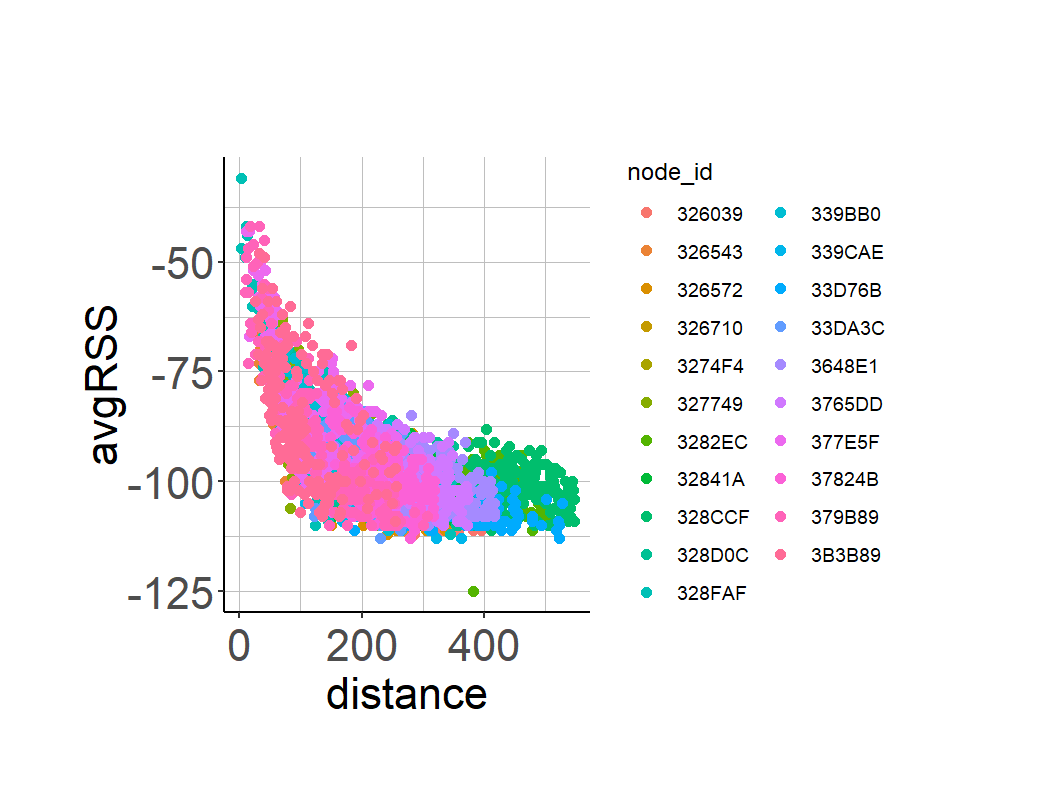
\includegraphics{images/multilateration_rss_vs_distance.png}
As distance increases, we see average RSS decreasing exponentially.

\subsection{Preliminary Exponential Decay Model - Determine starting values for the final model}\label{preliminary-exponential-decay-model---determine-starting-values-for-the-final-model}

\begin{itemize}
\tightlist
\item
  SSasvmp - self start for exponential model to find the data starting values
\item
  Asvm - horizontal asymptote (when large values) - y values decay to this value
\item
  R0 - numeric value when avgRSS (i.e., response variable) = 0
\item
  lrc - natural logarithm of the rate constant (rate of decay)
\end{itemize}

\begin{Shaded}
\begin{Highlighting}[]
\CommentTok{\# preliminary model {-} non{-}linear sampling}
\NormalTok{exp.mod }\OtherTok{\textless{}{-}} \FunctionTok{nls}\NormalTok{(avgRSS }\SpecialCharTok{\textasciitilde{}} \FunctionTok{SSasymp}\NormalTok{(distance, }
\NormalTok{                                Asym, }
\NormalTok{                                R0, }
\NormalTok{                                lrc), }
               \AttributeTok{data =}\NormalTok{ combined\_data)}

  \CommentTok{\# Summary of Model}
\FunctionTok{summary}\NormalTok{(exp.mod)}
  \CommentTok{\# rate of decay}
\FunctionTok{exp}\NormalTok{(}\FunctionTok{coef}\NormalTok{(exp.mod)[[}\StringTok{"lrc"}\NormalTok{]])}
\end{Highlighting}
\end{Shaded}

\subsection{Final Exponential Decay Model}\label{final-exponential-decay-model}

User provides self-starting values based on visualization of the data and values in the Preiliminary Model Output

exponential model formula: avgRSS \textasciitilde{} a * exp(-S * distance) + K

\begin{itemize}
\tightlist
\item
  a = intercept
\item
  S = decay factor
\item
  K = horizontal asymptote
\end{itemize}

\begin{Shaded}
\begin{Highlighting}[]
\DocumentationTok{\#\#  ***** Variables to define for final model below {-} replace values below with values from exp.mod ****  \#\# }
\NormalTok{a }\OtherTok{\textless{}{-}} \FunctionTok{coef}\NormalTok{(exp.mod)[[}\StringTok{"R0"}\NormalTok{]]}
\NormalTok{S }\OtherTok{\textless{}{-}} \FunctionTok{exp}\NormalTok{(}\FunctionTok{coef}\NormalTok{(exp.mod)[[}\StringTok{"lrc"}\NormalTok{]])}
\NormalTok{K }\OtherTok{\textless{}{-}} \FunctionTok{coef}\NormalTok{(exp.mod)[[}\StringTok{"Asym"}\NormalTok{]]}
  
  \CommentTok{\# Final Model}
\NormalTok{nls.mod }\OtherTok{\textless{}{-}} \FunctionTok{nls}\NormalTok{(avgRSS }\SpecialCharTok{\textasciitilde{}}\NormalTok{ a }\SpecialCharTok{*} \FunctionTok{exp}\NormalTok{(}\SpecialCharTok{{-}}\NormalTok{S }\SpecialCharTok{*}\NormalTok{ distance) }\SpecialCharTok{+}\NormalTok{ K, }
               \AttributeTok{start =} \FunctionTok{list}\NormalTok{(}\AttributeTok{a =}\NormalTok{ a, }
                            \AttributeTok{S =}\NormalTok{ S, }
                            \AttributeTok{K=}\NormalTok{ K), }
               \AttributeTok{data =}\NormalTok{ combined\_data)}

  \CommentTok{\# Model Summary}
\FunctionTok{summary}\NormalTok{(nls.mod)}

  \CommentTok{\# Model Coefficients }
\FunctionTok{coef}\NormalTok{(nls.mod)}

\DocumentationTok{\#\# Check the fit of the model and get predicted values}
  \CommentTok{\# Get residuals and fit of model and add variables to main table}
\NormalTok{combined\_data}\SpecialCharTok{$}\NormalTok{E }\OtherTok{\textless{}{-}} \FunctionTok{residuals}\NormalTok{(nls.mod)}
\NormalTok{combined\_data}\SpecialCharTok{$}\NormalTok{fit }\OtherTok{\textless{}{-}} \FunctionTok{fitted}\NormalTok{(nls.mod)}

  \CommentTok{\# Plot residuals by fit or distance}
\CommentTok{\#ggplot(combined\_data, aes(x = distance, y = E, color = node\_id)) +}
\CommentTok{\#        geom\_point(size = 2)}

\CommentTok{\#ggplot(combined\_data, aes(x = fit, y = E, color = node\_id)) +}
\CommentTok{\#  geom\_point(size = 2)}

  \CommentTok{\# Get model predictions}
\NormalTok{combined\_data}\SpecialCharTok{$}\NormalTok{pred }\OtherTok{\textless{}{-}} \FunctionTok{predict}\NormalTok{(nls.mod)}

\DocumentationTok{\#\# Plot with predicted line}
\FunctionTok{ggplot}\NormalTok{(combined\_data, }\FunctionTok{aes}\NormalTok{(}\AttributeTok{x =}\NormalTok{ distance,}
                          \AttributeTok{y =}\NormalTok{ avgRSS, }
                          \AttributeTok{color=}\NormalTok{node\_id)) }\SpecialCharTok{+} 
  \FunctionTok{geom\_point}\NormalTok{() }\SpecialCharTok{+}
  \FunctionTok{geom\_line}\NormalTok{(}\FunctionTok{aes}\NormalTok{(}\AttributeTok{y =}\NormalTok{ pred), }\AttributeTok{color=}\StringTok{"black"}\NormalTok{, }\AttributeTok{lwd =} \FloatTok{1.25}\NormalTok{) }\SpecialCharTok{+}
  \FunctionTok{scale\_y\_continuous}\NormalTok{(}\AttributeTok{name =} \StringTok{"RSS (dB)"}\NormalTok{) }\SpecialCharTok{+}
  \FunctionTok{scale\_x\_continuous}\NormalTok{(}\AttributeTok{name =} \StringTok{"Distance (m)"}\NormalTok{) }\SpecialCharTok{+}
  \FunctionTok{theme\_classic}\NormalTok{()}
\end{Highlighting}
\end{Shaded}

\begin{figure}
\centering
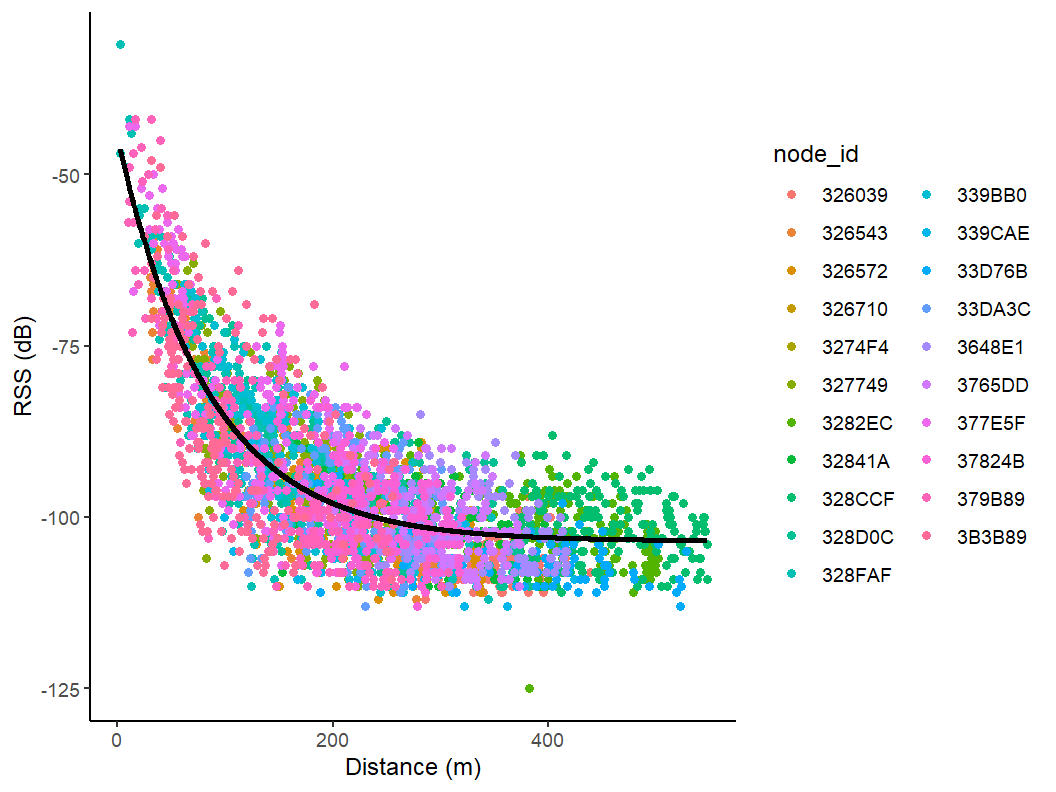
\includegraphics{images/multilateration_predicted_line.png}
\caption{RSS vs.~Distance with Predicted Line}
\end{figure}

\begin{Shaded}
\begin{Highlighting}[]
\NormalTok{a }\OtherTok{\textless{}{-}} \FunctionTok{unname}\NormalTok{(}\FunctionTok{coef}\NormalTok{(nls.mod)[}\DecValTok{1}\NormalTok{])}
\NormalTok{S }\OtherTok{\textless{}{-}} \FunctionTok{unname}\NormalTok{(}\FunctionTok{coef}\NormalTok{(nls.mod)[}\DecValTok{2}\NormalTok{])}
\NormalTok{K }\OtherTok{\textless{}{-}} \FunctionTok{unname}\NormalTok{(}\FunctionTok{coef}\NormalTok{(nls.mod)[}\DecValTok{3}\NormalTok{])}

\NormalTok{combined\_data }\OtherTok{\textless{}{-}} \FunctionTok{estimate.distance}\NormalTok{(combined\_data, K, a, S)}

\NormalTok{tile\_url }\OtherTok{=} \StringTok{"https://tile.openstreetmap.org/\{z\}/\{x\}/\{y\}.png"}
\NormalTok{testout }\OtherTok{\textless{}{-}}\NormalTok{ combined\_data[combined\_data}\SpecialCharTok{$}\NormalTok{TestId}\SpecialCharTok{==}\DecValTok{0}\NormalTok{,]}
\FunctionTok{leaflet}\NormalTok{() }\SpecialCharTok{\%\textgreater{}\%}
    \FunctionTok{addTiles}\NormalTok{(}
      \AttributeTok{urlTemplate =}\NormalTok{ tile\_url,}
      \AttributeTok{options =} \FunctionTok{tileOptions}\NormalTok{(}\AttributeTok{maxZoom =} \DecValTok{25}\NormalTok{)}
\NormalTok{    ) }\SpecialCharTok{\%\textgreater{}\%}
    \FunctionTok{addCircleMarkers}\NormalTok{(}
      \AttributeTok{data =}\NormalTok{ nodes,}
      \AttributeTok{lat =}\NormalTok{ nodes}\SpecialCharTok{$}\NormalTok{node\_lat,}
      \AttributeTok{lng =}\NormalTok{ nodes}\SpecialCharTok{$}\NormalTok{node\_lng,}
      \AttributeTok{radius =} \DecValTok{5}\NormalTok{,}
      \AttributeTok{color =} \StringTok{"cyan"}\NormalTok{,}
      \AttributeTok{fillColor =} \StringTok{"cyan"}\NormalTok{,}
      \AttributeTok{fillOpacity =} \FloatTok{0.5}\NormalTok{,}
      \AttributeTok{label =}\NormalTok{ nodes}\SpecialCharTok{$}\NormalTok{node\_id}
\NormalTok{    )  }\SpecialCharTok{\%\textgreater{}\%}
    \FunctionTok{addCircles}\NormalTok{(}
      \AttributeTok{data=}\NormalTok{testout, }
      \AttributeTok{lat =}\NormalTok{ testout}\SpecialCharTok{$}\NormalTok{node\_lat,}
      \AttributeTok{lng =}\NormalTok{ testout}\SpecialCharTok{$}\NormalTok{node\_lng,}
      \AttributeTok{radius =}\NormalTok{ testout}\SpecialCharTok{$}\NormalTok{distance,}
      \AttributeTok{color =} \StringTok{"red"}\NormalTok{,}
      \CommentTok{\#fillColor = "red",}
      \AttributeTok{fillOpacity =} \DecValTok{0}\NormalTok{)}
\end{Highlighting}
\end{Shaded}

\begin{figure}
\centering
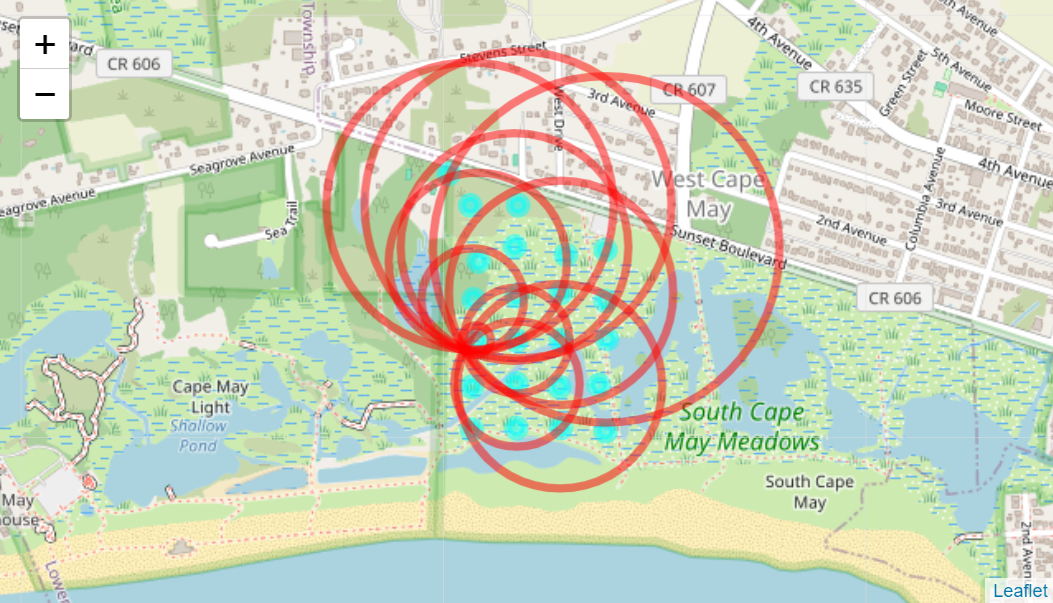
\includegraphics{images/multilateration_rings_map.png}
\caption{Ring Map}
\end{figure}

\begin{Shaded}
\begin{Highlighting}[]
\NormalTok{no.filters }\OtherTok{\textless{}{-}} \FunctionTok{trilateration.TestData.NoFilter}\NormalTok{(combined\_data)}
\NormalTok{RSS.FILTER }\OtherTok{\textless{}{-}} \FunctionTok{c}\NormalTok{(}\SpecialCharTok{{-}}\DecValTok{80}\NormalTok{, }\SpecialCharTok{{-}}\DecValTok{85}\NormalTok{, }\SpecialCharTok{{-}}\DecValTok{90}\NormalTok{, }\SpecialCharTok{{-}}\DecValTok{95}\NormalTok{)}
\NormalTok{RSS.filters }\OtherTok{\textless{}{-}} \FunctionTok{trilateration.TestData.RSS.Filter}\NormalTok{(combined\_data, RSS.FILTER)}
\CommentTok{\#DIST.FILTER \textless{}{-} c(315,500,750,1000)}
\CommentTok{\# Calculate error of location estimates of each test location when Distance filters are applied prior to trilateration }
\CommentTok{\#Dist.filters \textless{}{-} trilateration.TestData.Distance.Filter(combined\_data, DIST.FILTER)}

\NormalTok{SLIDE.TIME }\OtherTok{\textless{}{-}} \DecValTok{2}
\NormalTok{GROUP.TIME }\OtherTok{\textless{}{-}} \StringTok{"1 min"}

\NormalTok{test\_data }\OtherTok{\textless{}{-}}\NormalTok{ testdata }\SpecialCharTok{\%\textgreater{}\%}
  \FunctionTok{filter}\NormalTok{(time }\SpecialCharTok{\textgreater{}=} \FunctionTok{as.Date}\NormalTok{(}\StringTok{"2023{-}10{-}05"}\NormalTok{) }\SpecialCharTok{\&}\NormalTok{ time }\SpecialCharTok{\textless{}=} \FunctionTok{as.Date}\NormalTok{(}\StringTok{"2023{-}10{-}15"}\NormalTok{)) }\SpecialCharTok{\%\textgreater{}\%}
  \FunctionTok{filter}\NormalTok{(tag\_id }\SpecialCharTok{==} \StringTok{"2D4B782D"}\NormalTok{) }\SpecialCharTok{\%\textgreater{}\%}
  \FunctionTok{collect}\NormalTok{()}

\CommentTok{\# Function to prepare beep data for trilateration }
\CommentTok{\# by estimating distance of a signal based on RSS values}
\NormalTok{beep.grouped }\OtherTok{\textless{}{-}} \FunctionTok{prep.data}\NormalTok{(test\_data,}
\NormalTok{                          nodes,}
\NormalTok{                          SLIDE.TIME,}
\NormalTok{                          GROUP.TIME,}
\NormalTok{                          K, }
\NormalTok{                          a, }
\NormalTok{                          S) }

\NormalTok{RSS.filter }\OtherTok{\textless{}{-}} \SpecialCharTok{{-}}\DecValTok{95}
\NormalTok{location.estimates }\OtherTok{\textless{}{-}} \FunctionTok{trilateration}\NormalTok{(beep.grouped, nodes, RSS.FILTER)}

\CommentTok{\# this will take a while...}
\FunctionTok{mapping}\NormalTok{(nodes, location.estimates)}
\end{Highlighting}
\end{Shaded}


  \bibliography{doc.bib}

\end{document}
